%%%%%%%%%%%%%%%%%%%%%%%%%%%%%%%%%%%%%%%%%
% Thesis 
% LaTeX Template
% Version 1.3 (21/12/12)
%
% This template has been downloaded from:
% http://www.latextemplates.com
%
% Original authors:
% Steven Gunn 
% http://users.ecs.soton.ac.uk/srg/softwaretools/document/templates/
% and
% Sunil Patel
% http://www.sunilpatel.co.uk/thesis-template/
%
% License:
% CC BY-NC-SA 3.0 (http://creativecommons.org/licenses/by-nc-sa/3.0/)
%
% Note:
% Make sure to edit document variables in the Thesis.cls file
%
%%%%%%%%%%%%%%%%%%%%%%%%%%%%%%%%%%%%%%%%%

%----------------------------------------------------------------------------------------
%	PACKAGES AND OTHER DOCUMENT CONFIGURATIONS
%----------------------------------------------------------------------------------------

\documentclass[12pt, a4paper, oneside]{Thesis} % Paper size, default font size and one-sided paper

\graphicspath{{./Pictures/}} % Specifies the directory where pictures are stored
\usepackage{booktabs}
\usepackage{float}
\usepackage{cite}
\usepackage[square, numbers, comma, sort&compress]{natbib} % Use the natbib reference package - read up on this to edit the reference style; if you want text (e.g. Smith et al., 2012) for the in-text references (instead of numbers), remove 'numbers' 
\usepackage{color}
\lstset{frame=tb,
  language=python,
  aboveskip=3mm,
  belowskip=3mm,
  showstringspaces=false,
  columns=flexible,
  basicstyle={\small\ttfamily},
  numbers=none,
  numberstyle=\tiny\color{gray},
  keywordstyle=\color{blue},
  commentstyle=\color{dkgreen},
  stringstyle=\color{mauve},
  breaklines=true,
  breakatwhitespace=true
  tabsize=3
}

\definecolor{dkgreen}{rgb}{0,0.6,0}
\definecolor{gray}{rgb}{0.5,0.5,0.5}
\definecolor{mauve}{rgb}{0.58,0,0.82}
\hypersetup{urlcolor=blue, colorlinks=true} % Colors hyperlinks in blue - change to black if annoying
\title{\ttitle} % Defines the thesis title - don't touch this

\begin{document}
3
\frontmatter % Use roman page numbering style (i, ii, iii, iv...) for the pre-content pages

\setstretch{1.3} % Line spacing of 1.3

% Define the page headers using the FancyHdr package and set up for one-sided printing
\fancyhead{} % Clears all page headers and footers
\rhead{\thepage} % Sets the right side header to show the page number
\lhead{} % Clears the left side page header

\pagestyle{fancy} % Finally, use the "fancy" page style to implement the FancyHdr headers

\newcommand{\HRule}{\rule{\linewidth}{0.5mm}} % New command to make the lines in the title page

% PDF meta-data
\hypersetup{pdftitle={\ttitle}}
\hypersetup{pdfsubject=\subjectname}
\hypersetup{pdfauthor=\authornames}
\hypersetup{pdfkeywords=\keywordnames}

%----------------------------------------------------------------------------------------
%	TITLE PAGE
%----------------------------------------------------------------------------------------

\begin{titlepage}
\begin{center}

\textsc{\LARGE \univname}\\[1.5cm] % University name
\textsc{\Large Master Thesis}\\[0.5cm] % Thesis type

\HRule \\[0.4cm] % Horizontal line
{\huge \bfseries \ttitle}\\[0.4cm] % Thesis title
\HRule \\[1.5cm] % Horizontal line
 
\begin{minipage}{0.4\textwidth}
\begin{flushleft} \large
\emph{Author:}\\
\href{http://www.johnsmith.com}{\authornames} % Author name - remove the \href bracket to remove the link
\end{flushleft}
\end{minipage}
\begin{minipage}{0.4\textwidth}
\begin{flushright} \large
\emph{Supervisor:} \\
\href{http://www.jamessmith.com}{\supname} % Supervisor name - remove the \href bracket to remove the link  
\end{flushright}
\end{minipage}\\[3cm]
 
\large \textit{A thesis submitted in fulfilment of the requirements\\ for the degree of \degreename. 30 ECTS credits}\\[0.3cm] % University requirement text
\textit{.}\\[0.4cm]
%\groupname\\\deptname\\[2cm] % Research group name and department name
 
{\large \today}\\[4cm] % Date
%\includegraphics{Logo} % University/department logo - uncomment to place it
 
\vfill
\end{center}

\end{titlepage}

%----------------------------------------------------------------------------------------
%	DECLARATION PAGE
%	Your institution may give you a different text to place here
%----------------------------------------------------------------------------------------

%\Declaration{

%\addtocontents{toc}{\vspace{1em}} % Add a gap in the Contents, for aesthetics

%I, \authornames, declare that this thesis titled, '\ttitle' and the work presented in it are my own. I confirm that:

%\begin{itemize} 
%\item[\tiny{$\blacksquare$}] This work was done wholly or mainly while in candidature for a research degree at this University.
%\item[\tiny{$\blacksquare$}] Where I have consulted the published work of others, this is always clearly attributed.
%\item[\tiny{$\blacksquare$}] Where I have quoted from the work of others, the source is always given. With the exception of such quotations, this thesis is entirely my own work.
%\item[\tiny{$\blacksquare$}] I have acknowledged all main sources of help.
%\item[\tiny{$\blacksquare$}] Where the thesis is based on work done by myself jointly with others, I have made clear exactly what was done by others and what I have contributed myself.\\
%\end{itemize}
 
%Signed:\\
%\rule[1em]{25em}{0.5pt} % This prints a line for the signature
 
%Date:\\
%\rule[1em]{25em}{0.5pt} % This prints a line to write the date
%!TEX encoding = UTF-8 Unicode}

\clearpage % Start a new page

%----------------------------------------------------------------------------------------
%	QUOTATION PAGE
%----------------------------------------------------------------------------------------

\pagestyle{empty} % No headers or footers for the following pages

\null\vfill % Add some space to move the quote down the page a bit

\textit{``The end of a matter is better than its beginning; Patience of spirit is better than haughtiness of spirit."}

\begin{flushright}
Ecclesiates $7:8$
\end{flushright}

\vfill\vfill\vfill\vfill\vfill\vfill\null % Add some space at the bottom to position the quote just right

\clearpage % Start a new page

%----------------------------------------------------------------------------------------
%	ABSTRACT PAGE
%----------------------------------------------------------------------------------------

%\addtotoc{Abstract} % Add the "Abstract" page entry to the Contents

%\abstract{\addtocontents{toc}{\vspace{1em}} % Add a gap in the Contents, for aesthetics
%%We present two models of low temperature geothermal systems. In the first model, usually called lumped parameter modelling, an inverse problem is solved. Given a set of measured water level data , we find unknown parameters of the reservoir. The parameter of interest are reservoir production capacity and permeability between the reservoir boundary and it production part.\\
%%In the second model we derive the thermal front velocity induced during injection of colder water into a hot geothermal reservoir. We show that injection of cold fluid into a hot geothermal reservoir can be formulated as a Riemann problem for the conservation laws. The resulting thermal front velocity is derive, based on the unique Kruzkov entropy solution satisfying the Rankine-Hugoniot shock condition \cite{Risebro07}.\\ 
%%Our result is compared with the one obtained in \cite{SW} which is based on the conservation of energy and the characteristics method for solving conservation laws. Convergence test validate the numerical result obtained, and a difference of order $10^{-8}$ was observed between our result and the result obtained in \cite{SW}.
%%. \ldots
%%In geothermal energy extraction, injecting used fluid back to the reservoir is a resource management strategy. However a rapid cooling of the reservoir can occur when the cold injected fluid intersect the reservoir main fractures. It is therefore import to predict with accuracy thermal breakthrough by computing the cold water velocity.
%%In this thesis by using a nonlinear least square method, we present two scenarios for predicting water level changes in a reservoir: with injection and without injection. As anticipated injecting colder water in a reservoir mitigates pressure drawdown due to production.  Furthermore an analytical method is used to compute the cold front velocity induced. The cold front velocity obtained in this work is compared to the one obtained in \cite{Waj05}. A relative error of $10^{-3}$ was found between the two results. 
%
%}

\clearpage % Start a new page

%----------------------------------------------------------------------------------------
%	ACKNOWLEDGEMENTS
%----------------------------------------------------------------------------------------

\setstretch{1.3} % Reset the line-spacing to 1.3 for body text (if it has changed)

\acknowledgements{\addtocontents{toc}{\vspace{1em}} % Add a gap in the Contents, for aesthetics

I would like to say thank you to my supervisors for their patience, and all the faculties and staff in REYST who gave me the opportunity to complete this work \ldots
}
\clearpage % Start a new page

%----------------------------------------------------------------------------------------
%	LIST OF CONTENTS/FIGURES/TABLES PAGES
%----------------------------------------------------------------------------------------

\pagestyle{fancy} % The page style headers have been "empty" all this time, now use the "fancy" headers as defined before to bring them back

\lhead{\emph{Contents}} % Set the left side page header to "Contents"
\tableofcontents % Write out the Table of Contents

\lhead{\emph{List of Figures}} % Set the left side page header to "List of Figures"
\listoffigures % Write out the List of Figures

\lhead{\emph{List of Tables}} % Set the left side page header to "List of Tables"
\listoftables % Write out the List of Tables

%----------------------------------------------------------------------------------------
%	ABBREVIATIONS
%----------------------------------------------------------------------------------------

%\clearpage % Start a new page

%\setstretch{1.5} % Set the line spacing to 1.5, this makes the following tables easier to read

%\lhead{\emph{Abbreviations}} % Set the left side page header to "Abbreviations"
%\listofsymbols{ll} % Include a list of Abbreviations (a table of two columns)
%{
%\textbf{LAH} & \textbf{L}ist \textbf{A}bbreviations \textbf{H}ere \\
%\textbf{Acronym} & \textbf{W}hat (it) \textbf{S}tands \textbf{F}or \\
%}

%----------------------------------------------------------------------------------------
%	PHYSICAL CONSTANTS/OTHER DEFINITIONS
%----------------------------------------------------------------------------------------

%\clearpage % Start a new page

%\lhead{\emph{Physical Constants}} % Set the left side page header to "Physical Constants"

%\listofconstants{lrcl} % Include a list of Physical Constants (a four column table)
%{
%Speed of Light & $c$ & $=$ & $2.997\ 924\ 58\times10^{8}\ \mbox{ms}^{-\mbox{s}}$ (exact)\\
% Constant Name & Symbol & = & Constant Value (with units) \\
%}

%----------------------------------------------------------------------------------------
%	SYMBOLS
%----------------------------------------------------------------------------------------

%\clearpage % Start a new page

%\lhead{\emph{Symbols}} % Set the left side page header to "Symbols"

%\listofnomenclature{lll} % Include a list of Symbols (a three column table)
%{
%$a$ & distance & m \\
%$P$ & power & W (Js$^{-1}$) \\
% Symbol & Name & Unit \\

%& & \\ % Gap to separate the Roman symbols from the Greek

%$\omega$ & angular frequency & rads$^{-1}$ \\
% Symbol & Name & Unit \\
%}

%----------------------------------------------------------------------------------------
%	DEDICATION
%----------------------------------------------------------------------------------------

%\setstretch{1.3} % Return the line spacing back to 1.3

%\pagestyle{empty} % Page style needs to be empty for this page

%\dedicatory{For/Dedicated to/To my\ldots} % Dedication text

%\addtocontents{toc}{\vspace{2em}} % Add a gap in the Contents, for aesthetics

%----------------------------------------------------------------------------------------
%	THESIS CONTENT - CHAPTERS
%----------------------------------------------------------------------------------------

\mainmatter % Begin numeric (1,2,3...) page numbering

\pagestyle{fancy} % Return the page headers back to the "fancy" style

% Include the chapters of the thesis as separate files from the Chapters folder
% Uncomment the lines as you write the chapters
% Chapter 0

\chapter{Introduction} % Main chapter title

\label{Chapter1} % For referencing the chapter elsewhere, use \ref{Chapter1} 

\lhead{Chapter 1. \emph{Introduction}} % This is for the header on each page - perhaps a shortened title

In an increasing world population, energy consumption is directly linked to the survival of the human specie. 
With three quarter of the world energy source coming from fossil fuel in 2004 \cite{Beretta}, the world is subjected to an environmental crisis linked to our energy sources. The need for clean and renewable energy has never been important as it is today.
Geothermal energy classified as clean and sustainable energy has the potential of contributing significantly to sustainable energy use in many parts of the world \cite{Ax2005}. Generated by radioactive elements in the crust and lava within the earth, geothermal energy provides an unlimited source of energy for the world population. \\

Geothermal energy production at a sustainable rate can be maintained for $100-300$ years \cite{Ax2005, Axelsson2008}. This requires  knowledge and understanding of the geothermal system, sustainable production schemes such as reinjection of cold water and good management strategies. These strategies involve a multidisciplinary field of studies comprising geology, geophysics, chemistry and mathematics. With the development of modern computer architectures, numerical simulation combined with geological, geophysical and chemical data, play a key role in geothermal resource management.\\

Many pioneering works have been done in the field of geothermal engineering. Axelsson, Barker and Stefansson presented reinjection of water as a resource management strategy 
\cite{Ax2005, Axelsson2005, Ax-R08, Barker1995, Stefansson1997}. A method for analysing tracer test data used in reinjection was derived by Axelsson et. al \cite{Axelsson2005}. A lumped parameter modelling technique  was developed by Axelsson to simulate pressure response due to production in a low temperature geothermal system 
\cite{Ax-Rel-Lump05, Ax-Simul-Lump89}. Bjornsson developed the well bore simulator HOLA capable of simulating steady state two phase flow in a multi feed zones geothermal well \cite{Bjornsson1987}. Bodvarson was the first to derive an analytical method for calculating the thermal front velocity induced during injection of cold water in a hot geothermal reservoir for constant rock and fluid properties \cite{Bod-R72}. His method was latter extended for temperature independent rock and fluid properties by Stoppa et al and Achou \cite{Achou2013, Waj05}. \\

The main objective of this study is to present different methods used in modelling geothermal systems, in particular low temperature geothermal systems. volumetric and dynamic methods are presented. Reinjection is presented as an essential part of sustainable production  of geothermal energy. The lumped parameter modelling method is applied to a low temperature geothermal reservoir located in Munadarnes in west Iceland. The simulation reveals that the reservoir permeability is high. Multiple reinjection scenarios with different production and reinjection rate show that reinjection increases significantly the pressure of the reservoir. By using an analytical solution of water flow in a one dimension channel, the cooling response of the production well due to injection of cold water is presented. Cooling is minimised by placing the reinjection well at a few $km$ from the production well. By revisiting the work of Stoppa et. al \cite{Waj05}, an analytical method based on the theory of conservation laws is used to derived the thermal front velocity induced by reinjection.\\

The thesis is organised as follows: In chapter 2, properties of hydrothermal and geothermal systems are discussed. Hydrological and thermal properties of hydrothermal systems are presented. Geothermal systems are classified and methods for geothermal resource assessment are presented. In chapter 3, the thermal front velocity of cold water is derived using an analytical method.
 Chapter 4 present a case study using lumped parameters modelling. Chapter 5 contains conclusions and discussion and the possible extension or improvement of this work. 




%%----------------------------------------------------------------------------------------



%----------------------------------------------------------------------------------------

% Chapter 1

\chapter{Background} % Main chapter title

\label{Chapter1} % For referencing the chapter elsewhere, use \ref{Chapter1} 

\lhead{Chapter 1. \emph{Overview of geothermal systems}} % This is for the header on each page - perhaps a shortened title

%----------------------------------------------------------------------------------------
%\section{Introduction}
%Y-This is the introduction




\section{Hydrothermal system}
Hydrothermal systems can be defined as a set of processes that redistribute energy and mass in response to fluid circulation \cite{Norton1984}. Hydrothermal systems includes heat, fluid and sufficient permeability in the natural geological formation. The heat source is a magma chamber. Less frequently the source of heat is the crust with an abnormal high concentration of radioisotopes, mainly potassium 40, thorium 232, and uranium 235 and 230 \cite{springer}. The origin of the fluid is meteoric, that is rain water that percolates the ground, and frequently mixed with fluids and solutes of magnetic origin. In connection to geothermal energy, the most important properties of hydrothermal systems are given by rock and fluid properties. They are:
permeability, porosity and storage capacity \cite{Axelsson2008L}. The permeability represents viscous interactions between fracture surfaces and the fluid as it flows through interconnected fracture networks \cite{Norton1984}. Permeability expresses the ease at witch fluid flows through the medium. It is a qualitative property of the system, while porosity is a quantitative property described bellow.

\subsection{Hydrological properties}
the main hydrological property is porosity. Hydrothermal systems are mainly an interconnection of fracture. However, hydrothermal system can be approximated by porous medium \cite{Ax-Lecture08}.
\subsubsection{Porous medium}
A porous medium is a substance containing voids or pores, allowing fluid to be trapped or to flow throughout the medium. in the contest of geothermal energy, we are interested in the voids within the subsurface geological formation such as rock. To allow fluid flow, the pores spaces must form a network of interconnected voids space. Based on the time they were formed, the pores space can be divided in two, \cite{Bear88}. Original pore spaces are formed during the rock formation while secondary pore spaces are formed after the rock formation. Secondary porosity are due to physical and chemical changes occurring during the conversion of one rock type to an other. Porous medium can be classified based on their constituents. Intragranular porous medium created by voids within the rock grains and Intergranular porous medium formed by the voids between the rock grains. Fracture porosity is due to fractures within the rock caused by tensional forces. On the basis of mechanical properties, we can distinguish between consolidated porosity and unconsolidated porosity. In the consolidated case, the grains are kept together with a cementing material, while in the unconsolidated case the grains are loose, \cite{Bear88}. \\
Matrix porosity as a statistical measure of the voids spaces with respect to the total rock volume can be expressed as 

\begin{equation}
\Phi = \frac{V_{T}}{V_{T}} = 1-\frac{V_{S}}{V_{T}} \nonumber
\end{equation}

where 
\begin{equation}
V_{T}=V_{S}+V_{P} \nonumber
\end{equation}

is the total porosity, $V_{P}, V_{S}$ are the pore volume and solid (rock) volume respectively. In geothermal systems, only effective porosity is of importance, because it reflects interconnected pores and allow fluid to flow, \cite{Ax-Lecture08}. Effective porosity affects the storage capacity of the medium, which is its ability to absorb or release fluid in response of pressure change, due to fluid extraction or fluid injection in the medium. Alternatively we can define fracture porosity as the fraction of volume occupied by fractures.
\begin{figure}[htp] %  figure placement: here, top, bottom, or page
   \centering
   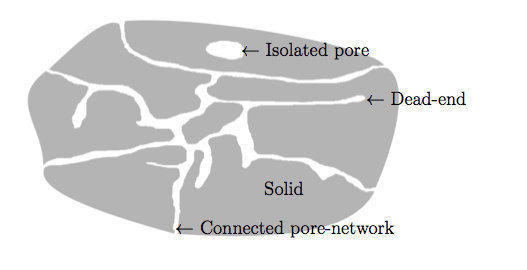
\includegraphics[width=4in]{porous.png} 
   \caption{A porous medium with connected network of pores, from \cite{Carina11}}
   \label{fig:porous}
\end{figure}

The recharge mechanism of porous medium are partly due to precipitation from the highland, that infiltrate the ground under gravity, filling up the interconnected pores spaces to form a saturation zone, \cite{Bear88}. When a part of the porous medium is trapped between impermeable formation, it is termed confined. Alternatively, an unconfined aquifer is bounded above by a water table. The movement of cold water in porous medium is described by Darcys law

\subsubsection{Darcy�s law}
Henry Darcy was a French hydraulic engineer interested in purifying water supplies using sand filters. He conducted experiments to determine the flow rate of water through the filters. Published in 1856, his conclusions have served as the basis for all modern analysis of ground water flow.The motion of cold water in porous medium is described by Darcy�s law:

\begin{equation}
Q = -K\frac{\rho}{\mu}(\Delta P-\rho g) \nonumber
\end{equation}

where 

\[
 K = \begin{bmatrix}
       K_{x} & 0 & 0           \\[0.3em]
       0 & K_{y} & 0 \\[0.3em]
       0 & 0 & K_{z}
     \end{bmatrix}
\]   
\\
\\
is the permeability tensor in 3 dimension. $Q (kg/sm^{2})$ is the fluid  flow rate, $\Delta P (Pa/m)$ the pressure gradient, $g$ acceleration of gravity and $\mu$ the fluid kinematic viscosity.  Darcy�s law stipulates that the motion of cold water in porous medium is due to the difference in pressure between two points and/or gravity forces. Capillarity pressure are pressure associated with low porosity, and can be neglected if we assume that fluid is flowing through the porous medium. Darcy�s law hold for laminar flow characterised by

\begin{equation}
R_{e}=\frac{Vd}{\nu},  \quad 1\leq R_{e} \leq 10 \nonumber
\end{equation}
where $d$ is the flow path diameter and $R_{e}$ the Reynolds number. Darcy�s law hold in porous medium but also in fracture medium, since large scale fracture medium can be approximated by porous medium, \cite{Ax-Lecture08}.
The pore velocity $v$ or the interstitial velocity is related to Darcy law by dividing the flow rate $Q$ by the porosity $\phi$. The pore velocity would be the velocity a conservative tracer would experience if carried by the fluid through the formation
\begin{equation}
v = \frac{Q}{\Phi} \nonumber
\end{equation}







\subsection{Thermal properties}
As mention before,  about $80 \%$ of the earth energy is generated by the decay of unstable  radio active elements in the crust and the mantle, \cite{Fowler05}. The major heat producing elements are  Uranium-238, Uranium-235, Potassium-40, and thorium-232 

 

\begin{table}[H]
\begin{center}
    \begin{tabular}{ | l | l | l | p{5cm} |}
    \hline
    elements & Heat generation $ (W/kg^{-1} )$ & Quatity $ (ppb) $ & Summary \\ \hline
    Uranium & $9.8.10^{-5} $& 15-25 & Uranium-238 produces $99 .28\%$ of the total Uranium energy. Uranium-235 produce $0.72\%$ of the total energy produce by Uranium. \\ \hline
    Thorium& $2.6.10^{-5}$ & 80-100 & Thorium-232 one out of $10^{4}$\\ \hline
    Potassium & $3.35.10^{19}$ & 150-260 & Potassium generate more energy  per kg. \\
    \hline
       % \caption{Heat producing radioactive elements \cite{Fowler05}}

    \end{tabular}
\end{center}
    \caption{Heat producing radioactive elements, \cite{Fowler05}}

\end{table}

The Crust generate 100 time more energy than the mantle per unit volume. However, the rate of energy generation for the entire earth is influenced by the mantle due to it large volume relatively to the crust, where the fifth of radioactive heat is generated. The total energy of the crust is about $1.4-2.7.10^{13} W$ \cite{Fowler05}. Due to low matrix and fracture  porosity, about 80 to 90$\%$ of this energy is stored in the rocks, \cite{Bod-R89}. 
%\subsubsection{Heat transfer within the earth}
The energy generated is mostly transfer through convection and  conduction. Radiation is ignored in modelling heat and mass extraction in hydrothermal systems. However, radiation plays an important role in shock wave propagation in hydrothermal systems. Hot fluid moves in the system through convective cells, where fractures are predominant. \\
consider a volume $V_{c}, V_{h}$ of cold and hot water respectively, and associated mass $m_{c}, m_{h}$. Assume that the fluid is heated bellow. The density of fluid is given by
 
\begin{equation} \label{eq:density}
\rho = \rho_{0}[1-\alpha(T-T_{0})+\beta(P-P_{0})]. \nonumber
\end{equation}
where  the compressibility 

\begin{equation}
\beta=-\frac{1}{\rho}\frac{d\rho}{dp}=-\frac{1}{V}\frac{dV}{dp} \nonumber.
\end{equation}

and $\alpha$ is the extensibility. The density decreases with increasing temperature, therefore

\begin{equation}
m_{h}=\rho_{h} V_{h} \le \rho_{c} V_{c}= m_{c}. \nonumber
\end{equation}
 
The column of hot water will rise when it is heated bellow. As it rises away from the heat source, it temperature decrease and the density of the fluid increase, allowing the column of cold water to fall. This create a convective cell. Many such cells are responsible for heat transfer in fractured porous medium. 

\begin{figure}[htp] %  figure placement: here, top, bottom, or page
   \centering
   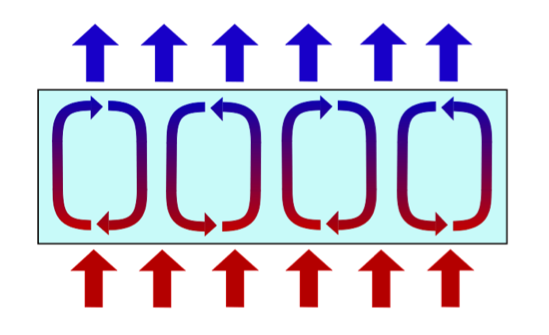
\includegraphics[width=4in]{cell.png} 
   \caption{A convective cell heated from bellow, from \cite{Carina11}}
   \label{fig:cell}
\end{figure}
When rock within the upper mantle and the crust are partially melted, the resulted molten lava, with lower density rises toward shallower depth in the form of magma chamber, dykes, or volcanics discharge, \cite{Pruess02}.\\
Conduction is predominant in sedimentary systems, where due to sediments packed together, fractures are more scarcer. in those systems, the microscopic particles undergoes constant oscillations and collisions. The energy generated by this chaotic movement create a temperature gradient causing heat to flow smoothly from region of higher temperature to region of low temperature. This is expressed by Fourier law
\begin{equation}
q = -k\Delta T
\end{equation} 
where $q, k, T$ are the heat flux, rock thermal conductivity and temperature respectively. Unlike conduction which generates smooth temperature field, radiation generate jump in the temperature field due to shock wave propagation.


    
%----------------------------------------------------------------------------------------




%____________________________________________________________________________________%%%%%%

\section{Geothermal Systems}
Geothermal energy can be defined as the outward energy flux of the earth, stored in the crust. The decay of unstable radio active elements such as Thorium, potassium and Uranium are for the most part responsible for this energy \cite{Fowler05}. Most geothermal systems are located along plate tectonics and are associated with volcanic regions. Due to a natural geothermal gradient within the crust, geothermal energy can a priori be found anywhere on earth.\\
\begin{figure}[htp] %  figure placement: here, top, bottom, or page
   \centering
   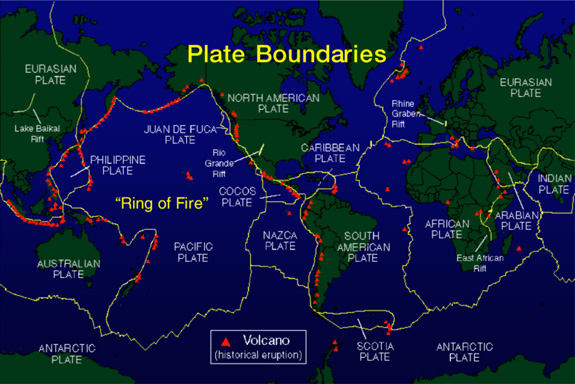
\includegraphics[width=4in]{plates.jpg} 
   \caption{Geothermal systems and plate boundaries}
   \label{fig:example}
\end{figure}

\\
A geothermal field is a geographical area with geothermal activity at the earth surface  \cite{Ax-Production08}. All hydrological systems directly related to geothermal resources such as fractures zone, heat source, aquifers etc... constitute the geothermal system. The geothermal reservoir is the permeable and hot part of the system \cite{Ax-Production08}.
Geothermal systems are classified on the basis of temperature (enthalpy) and their geological setting. 

\subsection{Classification based on temperature}
On the basis of temperature, geothermal systems can be classified as high temperature systems and low temperature systems. The temperature is at least $200\,^{\circ}{\rm c}$ in high temperature systems, while low temperature systems are characterised by temperature below $150\,^{\circ}{\rm c}$ \cite{Ax-Production08}.  The heat source in high temperature systems is often a hot intrusive magma, formed by incomplete melting of the upper mantle and the crust. High temperature systems are generally situated in volcanic regions. The heat source in low temperature systems, is the hot crust heated by radioactive elements.

\subsection{Classification based on geological formation}
On the basis of their geological setting, conventional geothermal systems can be classified as volcanic systems, convective systems, sedimentary systems, Engineered Geothermal Systems (EGS) and shallow geothermal systems \cite{Ax-Production08}.\\
\\
\emph{Volcanic systems} are located within or in the proximity of volcanic complexes. They  are high temperature systems and two phase flow (liquid and steam). The flow of water in volcanic systems is controlled by permeable fractures and fault zones  \cite{Ax-Production08}. The heat sources are hot intrusions or magma \cite{Ax-Production08}. \emph{Convective systems} are often situated outside volcanics complex and are predominantly low temperature systems. Characterised by highly fractured rocks heat is transferred within a convective system through convection cells. \emph{Sedimentary systems} are located in sedimentary basins characterised by permeable sedimentary layers. Heat is transfer mainly through conduction \cite{Ax-Production08}. An \emph{engineered geothermal system} generate geothermal energy without the need for natural convective hydrothermal resources. Through hydraulic stimulation, high pressure cold water is injected into the system, to enhance permeability in the naturally fracture rock. \emph{Shallow geothermal systems} refer to the thermal energy stored near the surface of the earth crust. This energy is utilised through heat pumps. \\
\\
Recently abandoned oil and gas wells or dry wells have been investigated for possible sources of geothermal energy.
Abandoned oil and gas wells are wells that ceased or never produced oil and gas. They can be as deep as 6000 $m$ \cite{Cheng2013}
In most geothermal project the cost of drilling can be as high as 50 $\%$ of the total project cost \cite{Bu2012}. By using abandoned oil and gas wells, the cost of geothermal energy production is reduced significantly. To produce geothermal energy from abandoned oil and gas wells, a double pipe heat exchanger is inserted into a well see Figure \ref{fig:ex}. \\
\begin{figure}[htbp] %  figure placement: here, top, bottom, or page
   \centering
   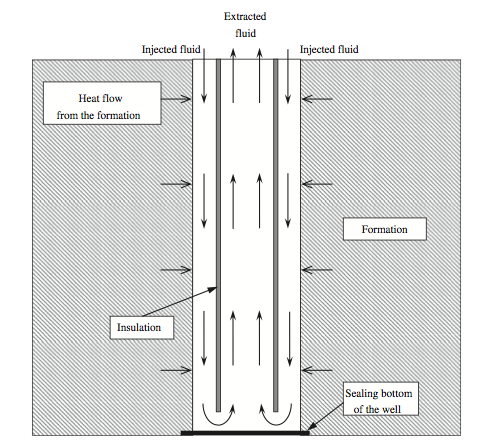
\includegraphics[width=4in]{doublep.png} 
   \caption{Diagram of a double pipe heat exchanger}
   \label{fig:ex}
\end{figure}
A working fluid is injected in one orifice of the heat exchanger. Due to the natural geothermal gradient, the fluid is heated by the geological formation. The recover geothermal energy depends on the flow rate of the injected working fluid and the geothermal gradient \cite{Bu2012, Cheng2013}. Computational simulation indicates that the fluid temperature can be around $130\,^{\circ}{\rm c}$ or more \cite{Bu2012}. Organic fluid such as isobutane can be used as working fluid. Due to their low boiling point they are easily converted into high temperature steam \cite{Cheng2013}.\\

%Geothermal energy from abandoned oil and gas wells is generated in a controlled environment. In the latter injected fluid in the geological formation can induce micro seismicity. On the other hand in abandoned oil and gas well, the fluid flow in a heat exchanger, reducing any risk of environmental hazards.
%%%%%%%%%%%%%%%%%%%%%%%%%%%%%%%%%%%%%%%%%%%%%%%%%%%%%%%%%%%%%



\subsection{Geothermal resource assessment methods}
Geothermal engineering is a multidisciplinary field of study. It includes numerical simulation, geophysics, geology and chemistry. The purpose of geothermal reservoir engineering is to estimate reservoir properties and production potential, simulate production response and estimate the size of geothermal resources. It plays a key role in resource management. Assessment methods in geothermal reservoir engineering are divided into two: Volumetric assessment method and dynamics assessment method \cite{Gudmundsdottir2012}. Volumetric assessment methods are used in the the first stage of a geothermal project and should be included in conventional geothermal monitoring programs \cite{Axelsson2008, Gudmundsdottir2012, Isor}. Volumetric method plays an integral role in geothermal resource management \cite{Axelsson2008}. It includes the use of geological, geophysical and chemical methods. Data from volumetric methods can be used to construct a conceptual model of the reservoir. The conceptual model is a descriptive model of the system. It incorporates the essentials physical features of the system such as heat sources, hot springs, permeable zones, boundary condition, recharge zones etc \cite{Osul01}. The conceptual model provides an estimate of the reservoir size and describes flow pattern within the system. It is the foundation for a successful numerical simulation. Volumetric method plays a key role during production. Dynamical methods includes simple analytical methods, details numerical simulations and lumped parameters modelling \cite{Gudmundsdottir2012}. A combination of volumetric methods and numerical simulation should enhance the reliability of mathematical model of geothermal systems \cite{Axelsson2000}


\subsubsection{Volumetric assessment methods}
\textbf{\underline{Geological methods}}\\
The most widely used method is geological mapping. It goal is to study the viability of a geothermal project. It includes geothermal surface manifestation mapping, surface petrology, mineralogy, lithology, tectonic. It also plays an import role in advanced stages of the project in well siting and well design. A map of surface thermal manifestation such as hot spring, mud pots and warm group can reveal if the geothermal field is active of extinct \cite{Isor}. \\
\\
\textbf{\underline{Geophysical methods}}\\
Geophysical methods are import part of geothermal resource assessment. Physical parameters such as density, resistivity and magnetism of the rock are measured. Gravity survey is used to measure the density variation, which can reveal dense intrusions.
Magnetic measurement can give information about dikes. Seismic surveys and seismic monitoring reveals fracture zones at depth \cite{Isor}. Gravimetric measurements may reveal tectonic features in the reservoir \cite{Isor}. Micro gravity monitoring can provide information on the net mass balance of the reservoir (difference between mass withdrawal and the recharge of water) \cite{Axelsson2000}. Mass balance from enlarging steam zones may also be seen from gravity monitoring \cite{Axelsson2000}.  Mass balance effect of reinjection may be detected by gravity monitoring \cite{ Axelsson2000}. Resistivity surveys reveals temperature distribution of the system and might help delineate cold fresh water inflow into the geothermal system \cite{Axelsson2000}. The commonly used resistivity survey are Transient ElectroMagnetic (TEM) and MagnetoTelluric (MT) sounding \cite{Isor}. 
\\
In TEM survey current is generated in a big loop laying on the ground. By induction the current produces a magnetic field in the ground. By turning off the current abruptly, the varying magnetic field in the ground induce a current. This current is used to map the resistivity structure of the upper most $1$ $km$ of the geothermal system \cite{Isor}.
\begin{figure}[H] %  figure placement: here, top, bottom, or page
   \centering
   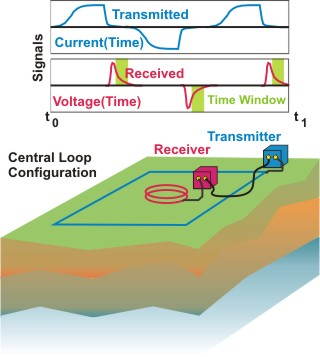
\includegraphics[width=2in]{tem.jpg} 
   \caption{TEM survey }
   \label{fig:tem}
\end{figure}
\\
The TM survey makes use of the natural fluctuation of the earth\�s magnetic field. By the principle of induction, the induced current in the earth is measured on the surface by two magnetics dipoles. Because the TM survey uses the natural magnetic field of the earth, it maps the resistivity structure of the geothermal system at greater depth, tens of $km$ \cite{Isor}.
\begin{figure}[H] %  figure placement: here, top, bottom, or page
   \centering
   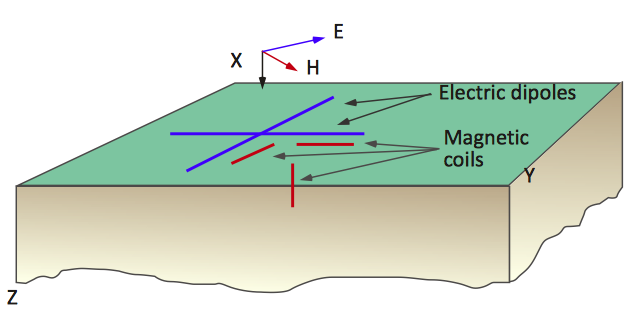
\includegraphics[width=4in]{tm.png} 
   \caption{TM survey}
   \label{fig:tm}
\end{figure}
 \\
\textbf{\underline{Chemical methods}}\\
Chemical composition of geothermal fluid (steam and water) can reveal the temperature of the reservoir. it plays an important role in anticipating corrosion and scaling in pipes and wells by identifying corrosive and scaling species. Chemical composition of the surface water reveals information about the recharge zone of a geothermal reservoir \cite{Isor}. Change in silica content of water production can be interpreted as inflow of cold water into the geothermal system \cite{Axelsson2000}.

\subsubsection{Dynamics assessment method}
\\
\textbf{\underline{Numerical simulation}}\\
Traditionally, conceptual models of geothermal systems are developed on the basis of information from various disciplines including geology, geophysics and geochemistry. Mathematical models are then applied to simulate the behaviour of the system using conceptual models \cite{Hagdu1995}.

On the basis of the conceptual model constructed from volumetric assessment methods, a careful mathematical model of the reservoir is constructed. Variables such as pressure, enthalpy, saturation, permeability, storage capacity are often simulated. A successful mathematical model is based on deep understanding of the physical and chemical processes of the system, the boundary condition, the fluid and rock properties, the location of sources and sinks  \cite{Osul01}. Fluid flow in geothermal systems can be approximated by flow in a porous medium. The flow is characterised both as single phase (water) with multi-component (carbon-dioxide and NaCl) or multi phase flow consisting of two phases, water and steam \cite{Hagdu1995}.
\\
Geothermal systems are modelled in terms of conservation of mass, momentum and energy. A complete model of the system should incorporate the flow of fluid in the reservoir and the production/reinjection wells \cite{Hagdu1995}. The general conservation equations for simulating two phase  flow in a geothermal reservoir are given by Grant \cite{Grant-Re82}:\\
\\
\textbf{Conservation of mass}
\begin{equation}
\phi\frac{ \partial  }{\partial t} \left ( \rho_{l}S_{l}f_{l}+  \rho_{g}S_{g}f_{g}   \right)+\nabla\cdot( \rho_{l}u_{l}f_{l}+ \rho_{g}u_{g}f_{g})+q_{m} = 0
\end{equation} 
where $\rho$, $S$  are the saturation and $f$ is the mass concentration of the chemical species in the fluid. $l$ and $g$ stand for liquid and gas (vapour). $u$ is given by equation (\ref{eq:cml},\ref{eq:cmg}). $q_{m}$ is the sink/source term $(kg)$ \\
\\
\textbf{Conservation of energy}
\begin{equation}
\phi\frac{ \partial  }{\partial t} \left ((1-\phi) \rho_{r}U_{r}+ \phi( \rho_{l}S_{l}U_{l} +\rho_{g}S_{g}U_{g} )   \right)+\nabla\cdot( \rho_{l}u_{l}h_{l}+ \rho_{g}u_{g}h_{g} -K\nabla T)+q_{E} = 0
\end{equation} 
$U$ is the internal energy, $h$ the enthalpy , $T$ the temperature, $K$ the heat conduction coefficient and $q_{E}$ the sink/source term $(J/m^{3}s)$.\\

%\clearpage
\textbf{Conservation of momentum}\\
The conservation of momentum is given by Darcys law. It describes a linear relationship between the fluid velocity and the pressure gradient relative to the rock:

\begin{equation}\label{eq:cml}
u_{l} = -\frac{kk_{rl}}{\mu_{l}}\nabla (P_{l}-\rho_{l}gz)
\end{equation}

\begin{equation}\label{eq:cmg}
u_{g} = -\frac{kk_{rg}}{\mu_{g}}\nabla (P_{g}-\rho_{g}gz)
\end{equation}
$k$ is the absolute permeability, and $k_{rl}$ and $k_{rg}$ are the relative permeabilities of the rock to the liquid and vapour phase respectively. The above equations hold assuming that capillary pressure effects are neglected.\\
\\

The steady state equation governing fluid flow in a vertical geothermal well is given by the mass, momentum and energy equation 
\cite{Bjornsson1987}
\begin{equation}
\frac{\partial m}{\partial z} = 0
\end{equation}

\begin{equation}\label{eq:cm}
\frac{\partial P}{\partial z}-\left(  \left( \frac{\partial P}{\partial z} \right)_{f}+ \left( \frac{\partial P}{\partial z} \right)_{a} + \left( \frac{\partial P}{\partial z} \right)_{p}     \right) = 0
\end{equation}

\begin{equation}\label{eq:ce}
\frac{\partial E}{\partial z}\pm Q= 0
\end{equation}

where $Q$ is the heat flow and $\left( \frac{\partial P}{\partial z} \right)_{f}, \left( \frac{\partial P}{\partial z} \right)_{a}, \left( \frac{\partial P}{\partial z} \right)_{p}$
are the pressure drop due to frictional, acceleration and potential forces along the well respectively. They are given respectively by

\begin{equation}\label{eq:f}
\left( \frac{\partial P}{\partial z} \right)_{f}= \varphi^{2}\left(    \frac{f_{lo}G^{2}}{4r_{w}\rho_{l}}   \right)
\end{equation}

\begin{equation}\label{eq:a}
\left( \frac{\partial P}{\partial z} \right)_{a} = G(xu_{g}+u_{l}(1-x))
\end{equation}

\begin{equation}\label{eq:a}
\left( \frac{\partial P}{\partial z} \right)_{p} = (\rho_{m})g
\end{equation}

$u_{l}$ and $u_{g}$ are the liquid and steam velocity, $\varphi^{2}$ is the two phase multiplier introduced by Martinelli and Nelson:
\begin{equation}
\varphi^{2} = 1+\left(\Gamma^{2}-1\right) \left(   B_{r}x(1-x)+x^{2}  \right)\nonumber
\end{equation}

\begin{equation}
\Gamma^{2} = \frac{\rho_{l}}{\rho_{g}} \nonumber
\end{equation}

\begin{equation}
B_{r} = B_{s}\left(         \frac{1}{2}\left(    1+\left(\frac{\mu_{g}}{\mu_{l}}\right)^{2}10^{-\frac{300\epsilon}{r_{w}}}   \right)\right)\nonumber
\end{equation}
$f_{lo}$ is the liquid friction factor and $B_{s}$ is given by Table \ref{table:bs}.

\begin{table}[H]

\centering
\caption{Different values of $B_{s}$ based on $\Gamma$ and $G$}
\label{table:bs}
\begin{tabular}{llr}

\toprule
%\multicolumn{2}{c}{Values $\Gamma, G, B_{s}$} \\
%\cmidrule(r){1-2}
$\Gamma$    & $G(\frac{kg}{m^{2}s})$ & $B_{s}$  \\
\midrule
$\leq9.5$      & $\leq 500$    & $4.8$      \\
\\
                       & $ 500\leq G \leq 1900$        & $\frac{2400}{G}$       \\
                       \\
                       &$\geq 1900$   &   $\frac{55}{G^{0.5}}$   \\
                       \\
  \hline   
  \\                                                                           
$9.5<\Gamma<28 $    & $\leq 600$     &  $\frac{520}{\Gamma G^{0.5}}$      \\
\\
                                        & $>600$     &  $\frac{21}{\Gamma}$      \\
                                        \\
  \hline    
  \\                             
$\geq 28$ &       &  $\frac{15000}{\Gamma ^{2}G^{0.5}}$     \\
\bottomrule
\end{tabular}
\end{table}

\begin{equation}\label{eq:energy}
E = m(   xh_{g} +(1-x)h_{l}+0.5(xu^{2}_{g}+(1-x)u^{2}_{l}) +g(L_{w}-z)       )
\end{equation}

For constant mass flow rate $m$ (\ref{eq:cm}, \ref{eq:ce}) can be solved for pressure $P$ and steam quality $x$ by using Newton method for system of nonlinear equations.\\
 \\
Equations governing the behaviour of a geothermal system can be solve numerically by various softwares.
Softwares for geothermal systems simulation fall into two categories: Reservoir and wellbore simulation software. The widely reservoir simulator are THOUGH and its family, STAR and TETRAD \cite{Pritchett1995, Pruess1999, Vinsome1993, Gudmundsdottir2012}. THOUGH family are designed to simulate the coupled transport of fluid, heat and chemical species for multi phase flow in porous and fracture media \cite{Pruess1999}. The conservation equations are discretised in space using the integral finite difference method \cite{Edwards1972, Narasimhan1976, Hagdu1995}.  The time derivative is discretised using a finite difference scheme (backward, forward, centered). Due to the fact that THOUGH is discretised using an integral finite difference method, it has the advantage of handling unstructured mesh as opposed to STAR and TETRAD. This makes THOUGH the facto reservoir simulation software \cite{Gudmundsdottir2012}\\
\begin{figure}[H] %  figure placement: here, top, bottom, or page
   \centering
   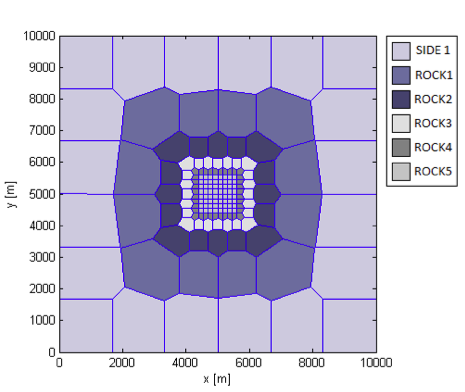
\includegraphics[width=4in]{mesh.png} 
   \caption{Unstructured mesh generated by THOUGH2. Taken from \cite{Gudmundsdottir2012}}
   \label{fig:example}
\end{figure}
The first wellbore softwares were designed to solve steady state conservation equation \cite{Gould1974, Gudmundsdottir2012}. The first simulator capable of handling unsteady state conservation equation was WELBORE designed by Miller \cite{Gudmundsdottir2012, Miller1980}. All these softwares solved the conservation equations from bottom to top along the well or vice versa, without incorporating the feed zones in the wells. The first software able to handle one feed zone was the software BROWN \cite{Bilicki1981, Gudmundsdottir2012}. HOLA was the first simulator capable of handling multiple feed zones in the well \cite{Bjornsson1987}.\\
\\

A successful geothermal systems simulation is based coupling empirical data and numerical simulation. The verification process map the measured data from the system to the result obtained from mathematical modelling. Verification is done through calibration \cite{Osul01}.  If the error between the measured and the calculated solution falls within an acceptable range, the simulation is a success. In this case the mathematical model represents a fairly good approximation of the system.
%\begin{figure}[H] %  figure placement: here, top, bottom, or page
%   \centering
%   %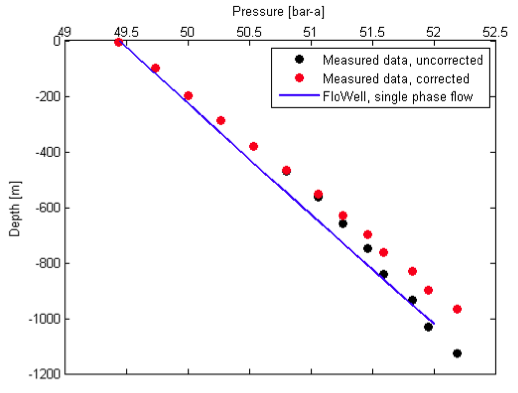
\includegraphics[width=2.5in]{val1.png} 
%      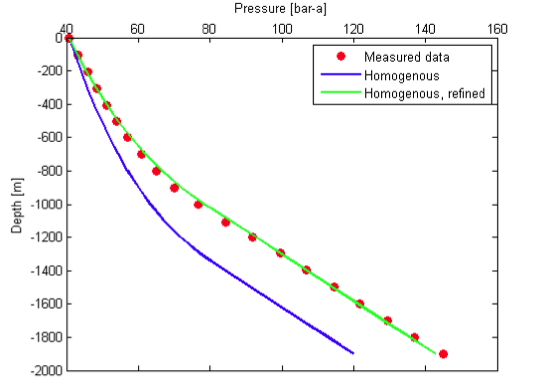
\includegraphics[width=4in]{val2.png} 
%   \caption{Verification process. Taken from (aldora)}
%   \label{fig:val}
%\end{figure}
Osulavan developed a general method of model calibration \cite{Osul01}. It consists of natural state modelling followed by history matching. In natural state modelling, the model is run for a long period of time to mimic the natural behaviour of the system. The simulated variables are compared with the measured field data. Some parameters of interest such as permeability structure, location of the heat source of the model are adjusted to obtain the minimum possible discrepancy between measured and simulated data. This step does not take into account the production history of the system. For system with production history, the measured behaviour of the geothermal field is matched with the simulated behaviour in response to production \cite{Osul01}. \\
\\
\textbf{\underline{Lumped parameters modelling and analytical method}}\\

A lumped parameter modelling software was designed by Axellsson to simulate the pressure change in a low temperature geothermal well \cite{Ax-Simul-Lump89}. The methods consist of approximating the permeability and the storage capacity of the reservoir by plumped parameters. By using inverse modelling the analytical response of the reservoir is mapped with measured data. Simple analytical method can also be used to model fluid flow in geothermal reservoir. In  Chapter (3) a case study using a lumped parameter modelling approach is presented. In chapter 4 a simple analytical method is used to predicts the thermal front velocity of injected cold water in a hot single phase geothermal reservoir.

%%%%%%%%%%%%%%%%%%%%%%%%%%%%%%%%%%%%%%%%%%%%%%%%%%%%%%%%%%%%%%%


\section{Reinjection in geothermal systems}
\subsection{Historical background and advantages}
Reinjection in geothermal resource management consist of reinjecting the used geothermal water back into the reservoir. Water of different origins such as  surface water and sewage water  can also be reinjected \cite{Ax-R08}. It started as a way on disposing the wast water from geothermal energy utilisation \cite{Ax-R08}. The first recorded instance of injection of cold water into a high temperature reservoir is in Ahuachapan field in El Salvador in 1969 \cite{Ax-R08, Stefansson1997}. At the same time a long term reinjection was used  successfully in the Dogger limestone reservoir located in the Paris basin \cite{Ax-R08}.  The Dogger reservoir stretching $150000 km^{2}$ is mainly used for district heating. The production and reinjection wells are separated by a distance of about $1km$. The reinjection scheme in the Paris basin lasting $30$ to $40$ years has indicated no significant cooling of the reservoir due to cold water injection \cite{Ax-R08}.
In 1970, operators in the Geyser geothermal field started to inject the steam condensate, and realised that this process increased the reservoir performance \cite{Ax-R08}. Since then reinjection has been an integrant part of resource management in the Geyser field. It was latter observed that due to injection, the decline of electrical production in the geyser was considerably slow \cite{Ax-R08, Stark2005}.
\\
In Italy reinjection started in 1974 at Lardelerollo field as a means to dispose the steam condensate \cite{Ax-R08, Capetti1995, Stefansson1997}. Long term production history has revealed that since reinjection started, steam production along with pressure have increased in the Lardelerollo geothermal field \cite{Ax-R08, Stefansson1997}, See Figure \ref{fig:lard}. 

\begin{figure}[H] %  figure placement: here, top, bottom, or page
   \centering
   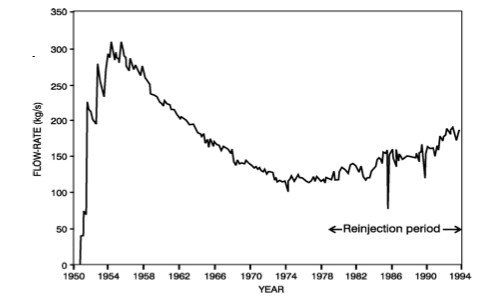
\includegraphics[width=4in]{lard.png} 
   \caption{Flow rate history at the Lardelorro field \cite{Capetti1995}. Taken from \cite{Ax-R08}}
   \label{fig:lard}
\end{figure}
 Reinjection sarted in Iceland in 1997 at the Laugaland low temperature field in north Iceland \cite{Axelsson2000}. In the Laugaland geothermal system 20 to 20$\%$ of the extracted mass are reinjected \cite{Axelsson2000, Ax-R08}. In the Hofstadir geothermal system in West Iceland reinjection started in 2006. About 40 to 50$\%$ of the extracted mass are reinjected back into the system \cite{Ax-R08}. Due to the low chemical content in most Icelandic geothermal field and the good recharge of water, reinjection started relatively late in Iceland \cite{Ax-R08}. Now reinjection is practiced in most of the hight temperature field in Iceland. It is estimated that the number of geothermal field in which reinjection is a part of resource management is likely more than 60 \cite{Ax-R08}. \\
 \\
 Reinjection is a vital part of an Enhanced Geothermal System (EGS) \cite{Ax-R08}. An EGS is a man made reservoir, created where there is hot rock but insufficient or little natural permeability or fluid saturation. About 80 to 90$\%$ of the energy of a geothermal reservoir is stored in the rock \cite{Ax-R08, Fowler05}. Therefore in an EGS, fluid is injected into the system at a sufficient pressure to create a fracture network into the rock with sufficient permeability. A production well is drilled into the fracture network to intersect the created flow paths. 
 
\begin{figure}[H] %  figure placement: here, top, bottom, or page
   \centering
   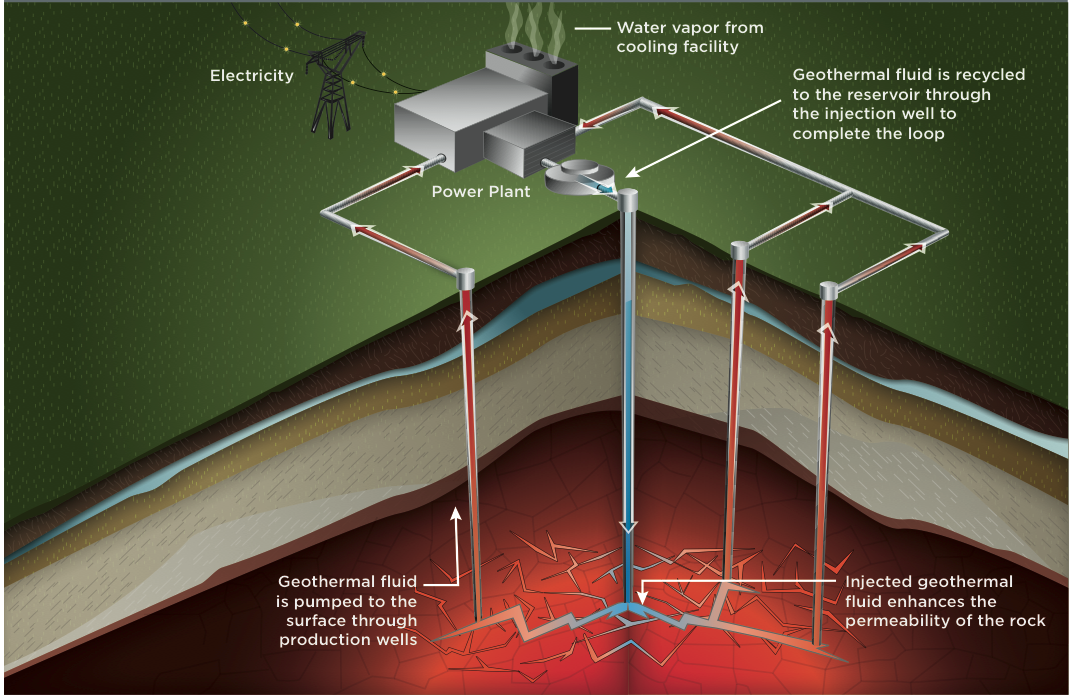
\includegraphics[width=5in]{egs.png} 
   \caption{schematic description of an EGS}
   \label{fig:egs}
\end{figure}

The production capacity of a geothermal system is controled by pressure response \cite{Ax-Production08}. During reinjection, the reservoir pressure is increased significantly, therefore reinjection increase the production capacity of the reservoir. As an environmental protection tool, it is a way of disposing the hight chemical content of geothermal wast water. It mitigates surface subsidence and maintains the integrity of surface activities \cite{Ax-R08}.\\
Reinjection can however affect the lifetime efficiency of the reservoir.  The lifetime efficiency of a reservoir can be defined as the ratio of the heat produced over it life time to the total available heat content of the reservoir \cite{Sayantan2012}. It can written as

\begin{equation}
\eta = \frac{E_{r}}{E_{T}} \nonumber
\end{equation}

where $\eta$ is the efficiency, $ E_{r}, E_{T}$ are the heat produced by the reservoir over it life time and the total available heat content respectively. The injected water is generally colder than the reservoir rock and can intersect fractures to create a premature cold water inflow and cool down the reservoir and decrease the reservoir efficiency. Reinjection can create and reopen pre-existing fractures. If created or reopen fractures intersect a cold aquifer, cold water breakthrough can be induced into the reservoir. Due to a large amount of fluid being injected into the reservoir, pressure increase can cause rock to slip along pre-existing fractures and produce microseismic events. Silica scaling in high temperature system, carbonate scaling in low temperature system and corrosion in pipelines and injection wells can be problems associated with injection. clogging of acquirers next to injection wells in sandstone reservoir can also be a significant problem \cite{Ax-R08}.
To mitigate the problems associated with reinjection , a careful reinjection scheme must be designed. 

\subsection{Mitigating problems associated with reinjection}
The main goals of reinjection can be summarise as follow:\\
1) Counteract pressure decline due to production\\
2) Maximise the reservoir efficiency by increasing the heat production over the life time of the reservoir\\
3)Environmental protection scheme\\
\\
If the purpose is option 3, injection wells can be placed outside the main production field without any direct hydrological connection \cite{Ax-R08}. If the purpose of the reinjection scheme is option 1 and 2, the rejection wells must be located inside the main production reservoir, in between production wells or on the outskirts of the reservoir but still in direct hydrological connection \cite{Ax-R08}. To avoid premature thermal breakthrough and increase the efficiency of the reservoir through injection, the injection scheme must ensure the optimum distance between injection wells and production wells \cite{Ax-R08, Sayantan2012}. Thermal breakthrough have been observed in relatively few geothermal systems worldwide \cite{Ax-R08, Stefansson1997}.  In the Palinpinon geothermal system in the Philippines, thermal breakthrough occur about $18$ months after reinjection started. The temperature dropped by about $50\,^{\circ}{\rm c}$ over a period of $4$ years \cite{Ax-R08}. Tracer tasting can be done to locate  fracture zones, flow path and determine the thermal front velocity to predict any premature thermal breakthrough. Analytical method can also be used the determined thermal front velocity. In chapter 4, an analytical method to determine thermal front velocity is presented.

\subsubsection{Tracer testing}
Tracer tests are the most powerful tool for studying connections between injection and production wells and predict thermal breakthrough \cite{AxelssonF2001}. It involves injecting a chemical tracer into the geothermal system, and monitor its recovery through time at various points.The chemical tracer arrival time and the thermal breakthrough time are proportional by $2-3$ order of magnitude \cite{Ax-R08}. Therefore determining the tracer arrival time gives the thermal breakthrough time. Three types of tracer are commonly used in geothermal application: Radioactive tracers such as Iodine-125, Iodide-131, Tritium etc, Fluorescent tracer such as rhodamin WT, chemical tracer such as iodide, bromide etc \cite{Axelsson2005}.\\ 
Assuming that a tracer of mass $M$ is injected at $t=0$ with injection rate $q$ into a one dimensional channel with cross sectional area $A$, porosity $\phi$ and fluid density $\rho$, 

\begin{figure}[H] %  figure placement: here, top, bottom, or page
   \centering
   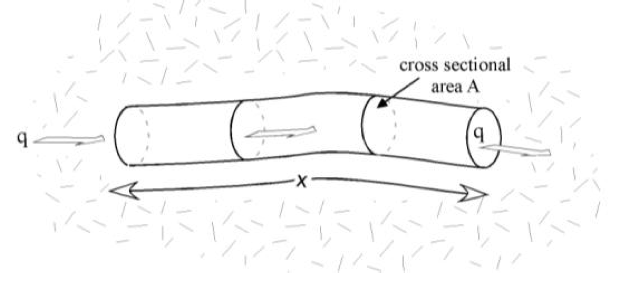
\includegraphics[width=4in]{chanel.png} 
   \caption{One dimensional flow channel connecting injection well and production well \cite{Axelsson2005}}
   \label{fig:example}
\end{figure}

The concentration $C$ of the tracer is modelled by \cite{Axelsson2005}:
\begin{equation}\label{eq:t}
\frac{\partial C}{\partial t}+u\frac{\patial C}{\partial x}-D\frac{\partial^{2}C}{\partial x^{2}} = 0
\end{equation}
The theoretical response
\begin{equation}\label{eq:s}
C(t) = \frac{4M\pho}{Q} \frac{1}{2\sqrt{\pi Dt}}\exp\left(-\frac{x-4t}{4Dt}\right)
\end{equation}
is simulated with the tracer data to obtain the flow channel volumes $Ax\phi $ and the longitudinal dispersivity $\alpha_{L}$ \cite{Axelsson2005}. In equation (\ref{eq:t}, \ref{eq:s})  $ u = \frac{q}{\rho A\phi}$, $D=\alpha_{L}u$, $Q$ is the production rate of the production well.
\\
The software TRINIV included in the ICEBOX software package developed at Iceland geosurvey uses a non linear least squares fitting to simulate data and return the flow channel volumes and the dispersivity \cite{Axelsson2005}. Ones equation (\ref{eq:s}) is fully defined, the concentration profile $C(t)$ can be use to determine the arrival time of the tracer concentration. 
 




%----------------------------------------------------------------------------------------

% Chapter 4

\chapter{Thermal front velocity in geothermal systems} % Main chapter title

\label{Chapter2} % For referencing the chapter elsewhere, use \ref{Chapter4} 

\lhead{Chapter 2. \emph{Thermal front velocity in geothermal systems}} % This is for the header on each page - perhaps a shortened title

\section{Sumary}

The injection of cold fluid into hot geothermal reservoirs can be formulated in terms of conservation laws. The cold front velocity induced during injection has been computed by Stopa and Wajnarowski in \cite{Waj05}. Their result was obtained from conservation of energy and the method of characteristics, applied to an initial boundary value problem. This computed thermal front velocity is expressed as a weighted average of the derivative of the flux function. In this paper we present a new method for computing the thermal front velocity by solving the Riemann problem. We show that the unique solution of the Riemann problem moves at the speed equal to the thermal front velocity. This result is predicted by the theory of hyperbolic conservation laws and is computed from the Rankine-Hugoniot shock condition. It is expressed as the average value of the derivative of the flux function over the interval defined by the injected water temperature and the reservoir temperature. A relative error of magnitude $10^{-3}$ was observed between the two results .%and the upper bound error of our result converges at least $133\cdot10^{4}$ times faster to zero then the one obtained in \cite{Stopa-Wajnarowski-06}. Convergence rate of about 2 was found when validating the numerical integration.

\section{Introduction}
In geothermal energy extraction, reinjecting  colder fluid into a hot reservoir is an integral part of resource management \cite{Ax-R08, Ax-Production08}. Due to the cold temperature of the injected fluid, However, cooling of the production wells can occur, as observed in Beowawe, Nevada and the Geysers Geothermal reservoir in the US  \cite{Beall}, \cite{Ben}. To mitigate this cooling effect, predicting the velocity of the cold water movement, is an essential part of the reinjection scheme. Bodvarsson \cite{Bod-R72} derived the thermal front velocity for constant fluid and rock properties, using the characteristic method. This technique produces a non physical solution when the rock and fluid properties are temperature dependent.  By using the method of characteristics, Stopa and Wajnarowski solved an initial-boundary value problem for the conservation laws \cite{Waj05}. They derived the thermal front velocity using conservation of energy. \\
\\
By formulating the injection problem as the well-posed Riemann problem, we relied on the established theory of hyperbolic conservation laws. Rather than using the method of characteristics, we used the unique solution for the Riemann problem given in \cite{Risebro07}. This solution propagates at a speed equal to the thermal front velocity.

In this work we revisit the findings of Stopa and Wajnarowski in \cite{Waj05}. In particular we compare the thermal front velocity obtained in  \cite{Waj05} with the one predicted by the theory of hyperbolic conservation laws. 
%In geothermal energy extraction, reinjecting  colder fluid into the hot reservoir is an integral part of resource management \cite{Ax-R08}, \cite{Ax-Production08}. However due to cold injected fluid, Cooling of the reservoir can occur, as observed in Beowawe, Nevada and the Geysers Geothermal reservoir in the US  \cite{Beall}, \cite{Ben}.\\
%To mitigate this cooling effect, predicting the thermal front velocity (velocity of the cold water movement), is an essential part of reinjection scheme. \\Bodvarsson \cite{Bod-R72} derived the thermal front velocity for constant fluid and rock properties, using the characteristics method. This method reduce a partial differential equation to a family of ordinary differential equation along which the solution is constant \cite{Evan00}. However for temperature dependent fluid and rock properties this method produce non physical solution. 
% \\
%Stoppa and Wajnarowski computed the thermal front velocity for temperature dependent rock and fluid properties \cite{Waj05}. They solved an initial boundary value problem by using the method of characteristics. Since this method produce non physical solution, a discontinuity was inserted into to solution such that the energy of the system was conserved. From this conservation of energy, the cold front velocity was derived.\\
% 
%In this section we present a new method for computing the thermal front velocity by solving a Riemann problem. We show that the unique solution of the Riemann problem moves at the velocity equal to the cold front velocity. Our result is computed from the Rankine-Hugoniot shock condition and is easier to evaluate using numerical integration. A difference of $10^{-8}$ was observed between our result and the one obtained in \cite{Waj05}. The upper bound error associated to our result converge rapidly to zero then the upper bound error associated to the one in \cite{Waj05} \\
%\\
%The rest of this chapter is organised as follow:
%In section 4.2 we lay down equations governing fluid flow in porous medium. Section 4.3 gives results from the theory of  hyperbolic conservation laws such as existence, and uniqueness of solution for the Riemann problem. In section 4.4 we derive the thermal front velocity for constant and temperature dependent rock and fluid properties. These derivation s are based on the theory of conservation laws from section 4.3
%


%Injection of cold fluid into a hot geothermal reservoirs can be formulated as conservation laws. The cold front velocity induced during injection has been computed by Bodvarsson \cite{Bod-R72} for constant rock and fluid properties by using the method of characteristic. This method reduce a partial differential equation to a family of ordinary differential equation along which the solution is constant \cite{Risebro07}. However for temperature dependent fluid and rock properties this method produce non physical solution. Stopa and Wajnarowski \cite{Waj05} computed the cold front velocity for temperature dependent fluid and rock properties. They solve an initial boundary value problem by using the characteristic method. Since the solution was non physical, they introduced a discontinuity at a point such that the energy of the system was conserved. From this conservation of energy, the thermal cold front velocity was derived. \\
%In this section we present a new method for computing the thermal front velocity by solving a Riemann problem. We show that the unique solution of the Riemann problem moves at the velocity equal to the cold front velocity. Our result is computed from the Rankine-Hugoniot shock condition and is easier to evaluate using numerical integration. A difference of $10^{-8}$ was observed between our result and the one obtained in \cite{Waj05}. The upper bound error associated to our result converge rapidly to zero then the upper bound error associated to the one in \cite{Waj05} \\
%
%In section 4.2 we lay down the equation governing fluid flow in porous medium. Section 4.3 gives some results from the theory of conservation laws such as existence, and uniqueness of solution for the Riemann problem. In section 4.4 we derive the thermal front velocity for constant and temperature dependent rock and fluid properties. These derivation are based on the theory of conservation laws from section 4.3
%


%%%%%%%%%%%%%%%%%%%%%%%%%%%%%%%%%%%%%%%%%%%%%%%%%%%%%%%%%%%%%%%%%%%%%%%%%%%%%%%%%%%%%%%%

\section{Governing equation}
A single phase(liquid) fluid flow in porous medium is given respectively by the conservation of mass and energy equation \cite{Woods}

\begin{equation}\label{eq:cm}
\frac{\partial (\phi \rho_{w}(u))}{\partial t} +\frac{\partial }{\partial x}(\rho_{w}(u)u_{w})=0
\end{equation}

\begin{equation}\label{eq:ce}
\phi\frac{\partial}{\partial t}\left (\phi \rho_{w}(u) c_{w}(u)u+(1-\phi)\rho_{r}(u) c_{r}(u)u\right) +\frac{\partial}{\partial x}(\rho_{w}(u) c_{w}(u) u_{w}u)=\lambda\frac{\partial^{2}u}{\partial x^{2}}
\end{equation}
\\
%-------------------------------------------------------------------------------------------------------------------------------------------------------------------------
where $u$ is the temperature, $c_{w}(u), c_{r}(u), \rho_{w}(u), \rho_{r}(u)$ are the heat capacity of water/rock and density of water/rock respectively. $\phi, u_{w}, \lambda$ are the porosity, the Darcy velocity of liquid phase and the heat conduction coefficient respectively. Darcy velocity $u_{w}$ is normally pressure dependent. Therefore equations (\ref{eq:cm}, \ref{eq:ce}) represent a system of two equations with two unknowns. \\
\\
To simplify the system of equations (\ref{eq:cm}, \ref{eq:ce}). we expend (\ref{eq:ce}) then use the conservation of mass (\ref{eq:cm}) to get one equation. See \cite{Waj05} for details. By expending (\ref{eq:ce}) we get

\begin{eqnarray}\label{eq:ce1}
c_{w}(u)u\left ( \frac{\partial \phi\rho_{w}(u)}{\partial t} +\frac{\partial }{\partial x}(\rho_{w}(u)u_{w})   \right ) + \frac{\partial }{\partial t}((1-\phi)\rho_{r}(u)c_{r}(u)u)\\ \nonumber
 + \phi\rho_{w}(u)\frac{\partial }{\partial t}(c_{w}(u)u) +  \rho_{w}(u)u_{w}\frac{\partial }{\partial x}(c_{w}(u)u) =\lambda\frac{\partial^{2}u}{\partial x^{2}}0 .
\end{eqnarray}

Using (\ref{eq:cm}), the first expression in (\ref{eq:ce1}) vanishes and we get
\begin{equation}\label{eq:ce2}
  \frac{\partial }{\partial t}((1-\phi)\rho_{r}(u)c_{r}(u)u) + \phi\rho_{w}(u)\frac{\partial }{\partial t}(c_{w}(u)u) +  \rho_{w}(u)u_{w}\frac{\partial }{\partial x}(c_{w}(u)u) =\lambda\frac{\partial^{2}u}{\partial x^{2}} .
\end{equation}
Applying the chain rule on (\ref{eq:ce2}) and assuming that Darcy velocity $u_{w}$ is constant, after rearranging the terms we end up with 
\begin{equation}\label{eq:cl}
\frac{\partial u}{\partial t} +\frac{u_{w}}{\phi}F(u)\frac{\partial u}{\partial x} =\left(\frac{\lambda}{  (1-\phi)\left( \frac{ \partial (\rho_{r}(u)  c_{r}(u) u) }{\partial u}\right) +  \phi \rho_{w}(u)\left(  \frac{\partial (c_{w}(u)u)  }{\partial u  } \right)     }\right)\frac{\partial^{2}u}{\partial x^{2}}%\frac{\partial u}{\partial t} +\frac{ \partial G }{\partial x}=0								       
\end{equation}

or 

\begin{equation}\label{eq:cl1}
\frac{\partial u}{\partial t} +\frac{ \partial G(u) }{\partial x}=\left(\frac{\lambda}{  (1-\phi)\left( \frac{ \partial (\rho_{r}(u)  c_{r}(u) u) }{\partial u}\right) +  \phi \rho_{w}(u)\left(  \frac{\partial (c_{w}(u)u)  }{\partial u  } \right)     } \right)\frac{\partial^{2}u}{\partial x^{2}}							       
\end{equation}
where 

\begin{equation}\label{eq:G0}
G(u) = \frac{u_{w}}{\phi}\int_{0}^{u}F(x)\mathrm{d}x \nonumber
\end{equation}
\begin{equation}\label{eq:F}
F(u)=\frac{  \phi \rho_{w}(u)\left(  \frac{\partial (c_{w}(u) u)  }{\partial u  }   \right)    }{  (1-\phi)\left( \frac{ \partial (\rho_{r}(u)  c_{r}(u) u) }{\partial u}\right) +  \phi \rho_{w}(u)\left(  \frac{\partial (c_{w}(u)u)  }{\partial u  } \right)     }
\end{equation}
 
 and from \cite{Waj05}
\begin{equation}
c_{w}(u)=\frac{1}{0.00023749816+8.0681767*10^{-8}u-8.0367134*10^{-10}u^{2}}\nonumber
\end{equation}
\\
\begin{equation}
c_{r}(u)=1234.257-454.546\exp(-0.00397334833482u)\nonumber
\end{equation}
\\
\begin{equation}
\rho_{w}(u)=1043.196-42.966623\exp(0.00689550122u)\nonumber
\end{equation}
\\
\begin{equation}
\rho_{r}(u)=\frac{2650}{1+(u-20)0.5*10^{-4}}.\nonumber
\end{equation}
\\

If we neglect conduction as second order effect by setting $\lambda=0$ in (\ref{eq:cl1}), we get 
\begin{equation}\label{eq:cl2}
\frac{\partial u}{\partial t} +\frac{ \partial G(u) }{\partial x}=0						       
\end{equation}
Equation (\ref{eq:cl2}) is a hyperbolic conservation laws and is the same equation derived in \cite{Waj05}. Function $G(u)$ is called the flux function of the scalar hyperbolic conservation laws. Equation (\ref{eq:cl2}) describe transport phenomenon. In this case transport of heat. Recall that $u=u(x,t)$ is the temperature and according to (\ref{eq:cl2}) the temperature is conserved. To see this, we can integrate over a given closed interval $[a,b]$ and get:
\begin{align}
\frac{\partial}{\partial t}\int_{a}^{b}u(x,t)\mathrm{d}x &=\int_{a}^{b}\frac{\partial}{\partial t}u(x,t)\mathrm{d}x\\
									      &=-\int_{a}^{b}\frac{ \partial }{\partial x}G(u(x,t))\mathrm{d}x\\
									      &=G(u(a,t))-G(u(b,t))\\
									      &=[inflow\quad at\quad a]-[inflow\quad at\quad b]
\end{align}
 Therefore the physical quantity modelled by $u$, is neither created nor destroyed: The total amount of $u$ contained inside any given interval $[a,b]$ can change only due to the flow of $u$ across boundary points $a, b$.
 \begin{figure}[H] %  figure placement: here, top, bottom, or page
    \centering
    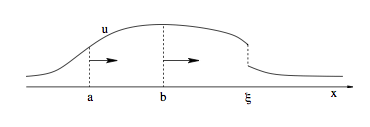
\includegraphics[width=4in]{cons.png} 
    \caption{Flow across point $a$ and $b$ with discontinuity at $\xi$}
    \label{fig:flow}
 \end{figure}
 
It is well known from the literature that equation of type (\ref{eq:cl2})  admit discontinuous solutions \cite{Risebro07}. Assume now that $u$ has a jump or discontinuity at $\xi$ see Figure \ref{fig:flow}. Then (\ref{eq:cl2}) is meaningful only in a class of discontinuous or generalised functions. Solutions must therefore be interpreted in distributional sense.
We therefore say that $u$ is a solution of (\ref{eq:cl2}) if

\begin{equation}\label{eq:weak}
\int\int( u\phi_{t}+G(u)\phi_{x})\mathrm{d}x\mathrm{d}t = 0
\end{equation}

for every infinitely continuous differentiable function $\phi$ with compact support. Equation (\ref{eq:weak}) is the weak formulation of (\ref{eq:cl2}). We only required that $u$ and $G(u)$ be locally integrable. This is a weaker requirement then continuity. To sum up, the problem of injecting colder water into a hot geothermal reservoir can be modelled by 
\begin{equation}\label{eq:cl3}
\frac{\partial u}{\partial t} +\frac{ \partial G(u) }{\partial x}=0			       
\end{equation}
with initial data
\begin{equation}\label{eq:i}
u(x,0)=u_{0}(x)						       
\end{equation}
This model assumed that the geological formation exhibit mainly micro permeability due to very small inter granular openings \cite{Bod-R72}. This mean that the reservoir is assumed homogeneous isotropic porous and permeable media, saturated with incompressible fluid. The fluid percolating through the reservoir rock. At any given point, the fluid and the reservoir have the same temperature.\\
This problem was first studied by Bodvarsson for temperature independent fluid and rock properties \cite{Bod-R72}. He found that the temperature field was transported through the porous media at a rate given by the thermal front velocity.

%Equation (\ref{eq:cl}) is a one dimension conservation laws, which can be solve with appropriate initial and/or boundary condition. In the next section, existence and unique of  (\ref{eq:cl}) is established.
%%%%%%%%%%%%%%%%%%%%%%%%%%%%%%%%%%%%%%%%%%%%%%%%%%%%%%%%%%%%%%%%%%%%%%%%%%%%%%%%%%%%%%%%






%\section{Shock wave theory for hyperbolic conservation laws}
%
%Let consider the initial value problem for Burgers equation
%\\
%\begin{equation}
%u_{t}+\left(  \frac{u^{2}}{2}\right)_{x}=0\quad in\quad \mathbb{R}\times(0,\infty), \quad u=g\quad on\quad \mathbb{R}\times(t=0)
%\end{equation}
%let the initial data $g$ be given by 
%%\begin{equation}
%\[ g(x) = \left\{ 
%  \begin{array}{l l }
%    1 & \quad \text{if $x\leq 0$ }\\
%    1-x & \quad \text{if $0\leq x\leq 1$ }\\
%    0 & \quad \text{if $x\geq 1$ }
%  \end{array} \right.\]
%%\end{equation}
%Applying the method of characteristics \cite{Evan00} the solution is given for $0\leq t\leq 1$ by 
%
%\[ u(x,t) = \left\{ 
%  \begin{array}{l l }
%    1 & \quad \text{if $x\leq t$ }\\
%    \frac{1-x}{1-t} & \quad \text{if $t\leq x\leq 1 $ }\\
%    0 & \quad \text{if $x\geq 1$ }
%  \end{array} \right.\]
%
%\begin{figure}[H] %  figure placement: here, top, bottom, or page
%   \centering
%   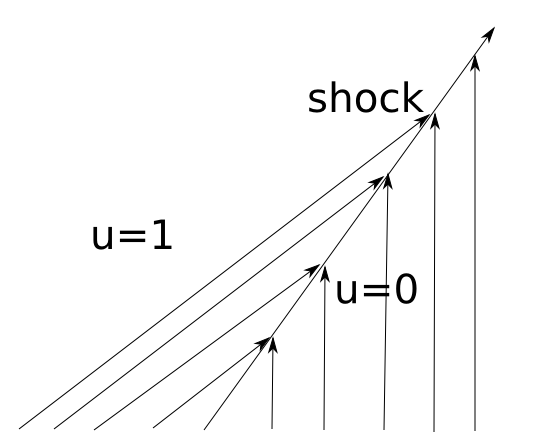
\includegraphics[width=2.5in]{sk.png} 
%   \caption{Shock wave propagation}
%   \label{fig:shock}
%\end{figure}
%
%For $t\geq 0$ the characteristics will cross and the solution is discontinuous. Now let the initial data $g$ be given by
%\[ g(x) = \left\{ 
%  \begin{array}{l l }
%    0 & \quad \text{if $x\leq 0$ }\\
%    
%    1 & \quad \text{if $x\geq 0$ }
%  \end{array} \right.\]
%
% then we can construct two solutions given by 
%\[ u_{1}(x,t) = \left\{ 
%  \begin{array}{l l }
%    0 & \quad \text{if $x\leq \frac{t}{2}$ }\\
%    
%    1 & \quad \text{if $x\geq \frac{t}{2}$ }
%  \end{array} \right.\]
%
%\[ u_{2}(x,t) = \left\{ 
%  \begin{array}{l l }
%    1 & \quad \text{if $x\leq t$ }\\
%    \frac{x}{t} & \quad \text{if $0<x< t$ }\\
%    0 & \quad \text{if $x< 0$ }
%  \end{array} \right.\]
%
%\begin{figure}[H] %  figure placement: here, top, bottom, or page
%   \centering
%   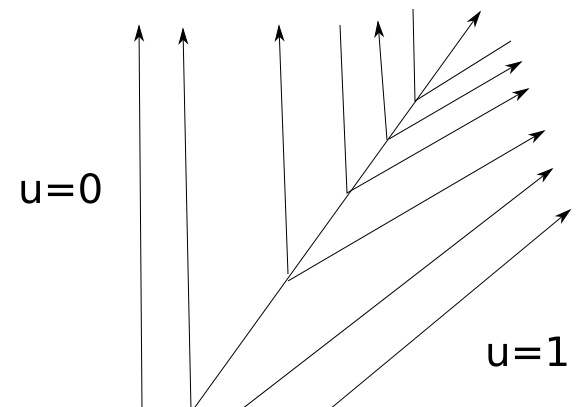
\includegraphics[width=2.5in]{u1.png} 
%   \caption{solution $u_{1}$ a non physical shock}
%   \label{fig:npshock}
%\end{figure}
%
%\begin{figure}[H] %  figure placement: here, top, bottom, or page
%   \centering
%   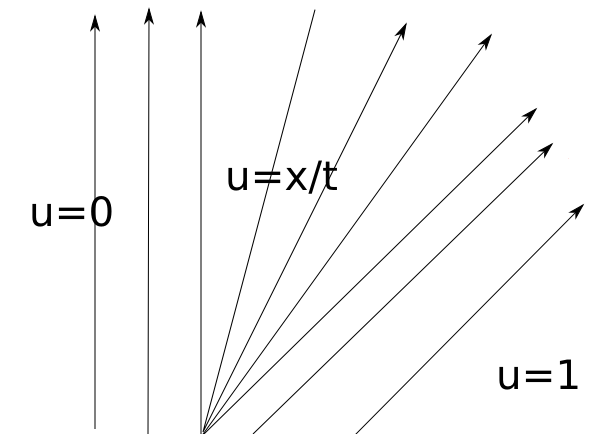
\includegraphics[width=2.5in]{u22.png} 
%   \caption{solution $u_{2}$, a rarefaction wave}
%   \label{fig:npshock}
%\end{figure}
%
%Our observation is that solutions of Burgers equation can have discontinuities with non physical shock formation. Given an initial data, the solution is not necessary unique. Under which condition can we have physical acceptable unique solution ? In the next section we set up different conditions under which the solution can be the unique physically acceptable solution.
%

%\subsection{Entropy condition and uniqueness of solution}
%The one dimension scalar conservation laws, with initial data is given by
%\\
%\begin{equation}\label{eq:conservationlaw}
%u_{t}=0\quad u(x,0)=u_{0}.
%\end{equation}
%\\
%Integrating (\ref{eq:conservationlaw}) between two points $x_{1}$ and $x_{2}$  we get
%\\
%\begin{align*}
%\frac{d}{dt}\int_{x_{1}}^{x_{2}} u(x,t)dx &=F(u(x_{1},t))-F(u(x_{2},t))\\
%                                                                   &=[inflow\quad at\quad x_{1}]-[outflow\quad at\quad x_{2}]. \nonumber
%\end{align*}
%\\
%Equation (\ref{eq:conservationlaw}) expresses the conservation of the quantity measured by $u$, since the rate of change of the amount of $u$ between $x_{1}$ and $x_{2}$ is given  by the difference in $F(u)$ evaluated at those points.This suggest that $F(u)$ should be interpreted as the flux of $u$ at the boundary points. In the theory of partial differential equation, it is common practice to seek weak solution then try to prove that the weak solution is differentiable. The differentiability of weak solution are expressed in term of weak derivatives. By following those steps, we start by laying down the weak formulation of the conservation law. This procedure is dictated by the physical phenomenon that (\ref{eq:conservationlaw}) model. As mention before conservations laws model shock wave propagation, and since shock waves induce discontinuity in the physical characteristics of the medium though which they propagate, one should expect the temperature profile of (\ref{eq:conservationlaw}) to be discontinuous.
%
%When $F(u)^{\prime}$ in (\ref{eq:conservationlaw}) dependent on temperature $u$, (\ref{eq:conservationlaw}) is non-linear, and continuous solutions do not exist. One is therefore forced to extend the solution set to generalized function or distribution (weak solution).\\
%A distribution $g$ is a continuous linear functional on $C_{0}^{\infty}$ (the space of infinitely differentiable function) such that for any family $\varphi_{n}$ $\in$ $C_{0}^{\infty}$ with supp$\varphi_{n}$ $\subseteq$ $K$, where $K$ is compact and such that all derivative satisfy $\varphi^{(m)}_{n}$ $\rightarrow$ $\varphi^{(m)}$ uniformly for some $\varphi$ $\in$ $C_{0}^{\infty}$, we have $g(\varphi_{n})$:= $\left <g,\varphi_{n}\right >$ $\rightarrow $ $\left <g,\varphi \right >$ . A function $\varphi$ $\in$ $C_{0}^{\infty}$ is generally called a test function.\\
%Our goal is to now give a formal definition of what it mean for $u$ to be a distribution or weak solution of (\ref{eq:conservationlaw}). Incorporating initial condition into the definition of weak solution, we define the partial derivative of a weak solution $u$ with respect to $t$ as:
%\begin{equation}\label{eq:weaks}
%\left<u_{t},\varphi\right>:=\int_{-\infty}^{\infty} u(x,0)\varphi(x,0)\mathrm{d}x -\left<u,\varphi_{t}\right>.
%\end{equation}
%And since the weak solution $u$ is defined for almost all $x$ and $t$, we get:
%\begin{eqnarray}
%  0& = & \left<0,\varphi \right> \nonumber \\
%   & = & \left<u_{t}+F(u)_{x},\varphi \right> \nonumber\\
%   & = & -\int_{-\infty}^{\infty}u(x,0)\phi(x,0)\mathrm{d}x-\left<u,\varphi_{t}\right>-\left<f(u),\phi_{t}\right> \nonumber \\
%   & = & \int_{-\infty}^{\infty}\int_{0}^{\infty}\left(u\varphi_{t}+F(u)\varphi_{x}\right) \mathrm{d}t \mathrm{d}x-\int_{-\infty}^{\infty}u(x,0)\varphi(x,0)\mathrm{d}x,
%\end{eqnarray}
%
%for all test function $\varphi$.\\
%The next definition gives a formal formulation of weak solution of the conservation laws.
%\begin{definition}
%Let $f:\mathbb{R} \longrightarrow \mathbb{R}$ be a smooth function. A measurable function $u=u(x,t)$, defined on an open set $\Omega \subseteq \mathbb{R}\times \mathbb{R}$ and with values in $\mathbb{R}$ is a weak solution or distributional solution of the conservation laws , if for every test function $\varphi :\Omega \longrightarrow \mathbb{R}$ with compact support, (\ref{eq:weaks}) is satisfied.
%\end{definition}
%Observe that no continuity assumption is made on the the weak solution $u$. The only requirement is that $u$ and $f$ be locally integrable: $u$, $f(u)$ $\in L_{loc}^{1}$.\\
% Next we investigate the type of weak solutions that satisfies (\ref{eq:weaks})). We keep in mind that our ultimate goal is to show that there exist a unique solution to the conservation law, and that this unique solution is stable with respect to the initial data. This last condition is very important for any physical application.\\
% 
 
 %%%%%%%%%%%%%%%%%%%%%%%%%%%%%%%%%%%%%%%%%%%%
%To prove uniqueness of solution a condition derived from physical experience called entropy condition must be imposed on equation (\ref{eq:conservationlaw})). This is done since there exist many solutions and we need to filter those solutions in order to capture the physical admissible one. Imposing an entropy condition on the conservation law lead to the so called Rankine-Hugoniot jump condition, which is an extra condition that a shock wave must posses. It gives the propagation speed of the shock wave across a discontinuity. We express all this formally as followed: we know that the physical problem that (\ref{eq:conservationlaw})) model has viscosity, and the conservation laws that is derive is the limit of the real physical phenomenon. The entropy condition is then called the viscous regularisation or \emph{traveling wave entropy condition} \cite{Risebro07}. Since the conservation laws is the limit of
%
%\begin{equation}\label{eq:viscousity}
%u_{t}^{\epsilon} + F(u^{\epsilon})_{x} = \epsilon u_{xx}^{\epsilon},
%\end{equation}
%as $\epsilon$ $\rightarrow$ $0$, where $\epsilon$ is nonnegative. Equation(\ref{eq:viscousity}) is well-posed classically, meaning that its exist a unique smooth solution and that the solution is stable with respect to the initial data. Suppose that the solution $u$ move with a speed $s$ across the discontinuity with a constant state:
%
%\begin{equation}
%u(x,t) = \left\{
%\begin{array}{rl}
%u_{l} & \text{if } x < st\\
%u_{r} & \text{if } x \geq st.
%\end{array} \right.
%\end{equation}
%
%Let $u^{\epsilon}=U((x-st)/ \epsilon)=U( \xi)$ be the solution of (\ref{eq:viscousity}). By definition, $u$ satisfy \emph{the traveling wave entropy condition} if $u(x,t)=u^{\epsilon}(x,t)=U(\xi)$ as $\epsilon$ goes to 0 pointwise.
%Now inserting $u^{\epsilon}$ into (\ref{eq:viscousity}) gives:
%\begin{equation}
%-s\dot{U}+\frac{dF(U)}{d\xi}=\ddot{U}.
%\end{equation}
%And integrating gives:
%
%\begin{equation}\label{eq:rankine}
%\dot{U}=-sU+F(U)+A.
%\end{equation}
%Since $u(x,t)$ satisfy the \emph{traveling wave entropy condition} we have:
%
%\begin{equation}
%U(\xi) = \left\{
%\begin{array}{rl}
%u_{l} & \text{if } x < st\\
%u_{r} & \text{if } x \geq st.
%\end{array} \right.
%\end{equation}
%as $\epsilon$ goes to 0, which yield $\dot{U(\xi)}=0$ as $\xi$ goes to infinity. Inserting this in (\ref{eq:rankine}) yield
%\begin{equation}\label{eq:rhugoniot}
%s(u_{l}-u_{r})=F(u_{l})-F(u_{r})
%\end{equation}
%which is the Rankine-Hugoniot jump condition. We formally express this in the following lemma.
%
%\begin{lemma}
%If the function $u=u(x,t)$ is the solution of the conservation laws with initial data,
%\begin{equation}
%u(x,0) = \left\{
%\begin{array}{rl}
%u_{l} & \text{if } x <0\\
%u_{r} & \text{if } x \geq0
%\end{array} \right.
%\end{equation}
%Then (\ref{eq:rhugoniot}) hold.
%\end{lemma}
%
%\begin{proof}
%See \cite{Risebro07}, page 9-11.
%Let $\varphi$ be a test function, and let $\Omega$ be a ball containing the support of $\varphi$. We consider the two domains:\\
%$\Omega^{+}=\Omega\cup \{x>st\}$, \quad $\Omega^{-}=\Omega\cup \{x<st\}$, where st is the line through the origin of the $(x,t)$ plane, separating $\Omega$ into $\Omega^{+}$ and $\Omega^{-}$. We introduce the vector field $\textbf{V}=(u\varphi, F(u)\varphi)$, so that,
%\begin{equation}
%\iint_{\Omega^{+}\cup\Omega^{-}}\nabla.\textbf{V}\mathrm{d}x\mathrm{d}t=0.
%\end{equation}
%Let $\textbf{n}^{+}$ and $\textbf{n}^{-}$ denote the outer unit normal to $\Omega^{+}$ and $\Omega^{-}$ respectively. Let $dS$ denote the differential of the arc length along the line $x=st$. We then have:\\
%$\textbf{n}^{+}dS=(s,-1)dt$,\quad\quad $\textbf{n}^{-}dS=(-s,1)dt$.\\ Applying Guauss theorem respectively to $\Omega^{+}$ amd $\Omega^{-}$, we get:
%
%\begin{equation}
%\begin{aligned}
%\iint_{\Omega^{+}\cup\Omega^{-}}\nabla.\textbf{V}\mathrm{d}x\mathrm{d}t&=\int_{\partial\Omega^{+}}\textbf{n}^{+}.\textbf{V}\mathrm{d}S+\int_{\partial\Omega^{-}}\textbf{n}^{+}.\textbf{V}\mathrm{d}S\\
%                                                                       &=\int\left[su_{r}-F(u_{r})\right]\varphi(st,t)\mathrm{d}t+\int\left[-su_{l}+f(u_{l})\right]\varphi(st,t)\mathrm{d}t\\
%                                                                       &=\int\left[s(u_{r}-u_{l})-F(u_{r})-F(u_{l})\right]\varphi\mathrm{d}t=0                                                                      
%\end{aligned}
%\end{equation}
%which implies (\ref{eq:rhugoniot}).
%\end{proof}
%An other entropy condition (condition derived from physical laws) called the \emph{Kruzkov entropy condition} is important in the sense that it incorporate the definition of weak solution, and is an important tool in proving the uniqueness of the conservation laws. It is given for the time interval $[0,T]$ in the integral form as followed:
%
%\begin{equation}
%\int_{0}^{T}\int_{-\infty}^{\infty}\left( \mid u-k \mid \varphi_{t}+q(u,k)\varphi_{x} \right) \mathrm{d}x \mathrm{d}t + \int \mid u(x,0)-k \mid \varphi(x,0) \mathrm{d}x  \geq 0 
%\end{equation}
%\\
%where $q(u,k)=sign(u,k)(F(u)-F(k))$, $k$ is a non negative constant and $\varphi$ is any non negative test function.
%We note that the \emph{traveling wave entropy condition} and the \emph{Kruzkov entropy condition} are equivalent for sufficiently smooth weak solution. We introduce a lemma which is needed to prove uniqueness.
%
%\begin{lemma} see,\cite{Risebro07}.
%let $h$ $\in$ $L^{\infty}(\mathbb{R\times R})$ with compact support. Assume that for almost all $x_{0} \in \mathbb{R}$ the function $h(x,y)$ is continuous at $(x_{0},x_{0})$. The following hold:
%\begin{equation}
%lim_{\epsilon \rightarrow 0}\int\int h(x,y)w_{\epsilon}(x-y)\mathrm{d}y\mathrm{d}x =\int h(x,y)\mathrm{d}x.
%\end{equation}
%\end{lemma}
%
%
%Now we are ready to prove the following theorem giving the uniqueness of solution.
%\begin{theorem} see \cite{Risebro07}.
%Assume that $F$ is Lipschitz continuous, and let $u$ and $v$ be two weak solutions of the initial value problems
%\begin{equation}
%u_{t}+F(u)_{x}=0 \quad u(x,0)=u_{0}
%\end{equation}
%\begin{equation}
%v_{t}+F(v)_{x}=0 \quad v(x,0)=v_{0}
%\end{equation}
%respectively satisfying the \emph{Kruzkov entropy condition} . Assume that $u_{0}-v_{0}$ is integrable and both $u$ and $v$ have finite total variation in $x$ for each $t$. Then
%\begin{equation}
%\mid\mid u(x,t)-v(x,t) \mid\mid_{1}\quad \leq\quad\mid\mid u_{0}-v_{0} \mid\mid_{1}
%\end{equation}
%In particular, if  $u_{0}=v_{0}$ then $u=v$.
%\end{theorem}
%
%\begin{proof}
%To prove \textbf{Theorem 2} we assume that there exist a constant $C$ such that the following is satisfy:
%
%\begin{equation}
%sup\frac{\mid F(u)-F(v)\mid}{\mid u-v\mid} \leq C
%\end{equation}
% For $u \neq v$. We assume also that $u$ and $v$ are of bounded variation in $x$ for each fixed $t$ that is 
% 
% \begin{equation}
% T.V.(u(.,t)),T.V.(v(.,t))<\infty
% \end{equation}
% 
% Where $T.V.(u)=sup \sum_{i}( u(x_{i})-u(x_{i-1}))$ and the supremum is taken over any finite partition. Consequently if $u$ is of bounded variation then $u$ is continuous almost every where in distribution. Now since $u$ and $v$ are weak solutions of the conservation laws, they satisfy the \emph{Kruzkov entropy condition (KEC)} . Assume also that the test function $\varphi$ is compactly supported in $t>0$, then KEC becomes:
%
% \begin{equation}
%\int_{0}^{t}\int_{-\infty}^{\infty}\left( \mid u-k \mid \varphi_{t}+q(u,k)\varphi_{x} \right) \mathrm{d}x \mathrm{d}t \geq 0 
%\end{equation}
%Now we use the method of doubling of variable. We double the variable of the test function $\varphi(x,t)$ to $\varphi(x,t,y,s)$ compact supported in $t>0$ and $s>0$. This smart choice of the test function $\varphi$ is important. Let $\psi(x,t)$ be an other test function with compact support in $t>\epsilon_{0}$ such that:
%\begin{equation}
%\varphi(x,t,y,s)=\psi\left(\frac{x+y}{2},\frac{t+s}{2}\right)w_{\epsilon_{0}}(t-s)w_{\epsilon}(x-y)
%\end{equation}
%And we get:
%
%\begin{equation}
%\varphi_{t}+\varphi_{s} = \psi_{t}\left(\frac{x+y}{2},\frac{t+s}{2}\right)w_{\epsilon_{0}}(t-s)w_{\epsilon}(x-y)
%\end{equation}
%
%
%\begin{equation}
%\varphi_{x}+\varphi_{y} = \psi_{x}\left(\frac{x+y}{2},\frac{t+s}{2}\right)w_{\epsilon_{0}}(t-s)w_{\epsilon}(x-y)
%\end{equation}
%
%Since both $u$ and $v$ satisfies the \emph{Kruzkov entropy condition}, we set $k=u(x,t)$ in the expression for $u$ and $k=v(y,s)$ in the expression for $v$ in the KEC formulation, and this gives us:
%
%\begin{equation}
%\iiiint(\mid u(x,t)-v(y,s) \mid(\varphi_{t}+\varphi_{s})+q(u,v)(\varphi_{x}+\varphi_{y}))\mathrm{d}x\mathrm{d}t\mathrm{d}y\mathrm{d}s \geq 0
%\end{equation}
%
%Assume now that $\psi$ is supported in $t>\epsilon$, and we want to apply \textbf{lemma1} respectively to $h(x,t)=\mid u(x,t)-v(y,s)\mid w_{\epsilon_{0}}(\phi_{t}+\phi_{s})$ and $h(x,y)=q(x,y)w_{\epsilon_{0}}(\phi_{x}+\phi_{y})$, this is justify since we fix $t$ and $s$, and therefore $u$ and $v$ are only functions of $x$ and $y$. Now by letting $\epsilon_{0}$ and $\epsilon$ goes to 0 and applying \textbf{lemma 2}, we get
%
%\begin{equation}
%\iint(\mid u(x,t)-v(x,t)\mid \psi_{t} +q(u,v)\psi_{x}) \geq 0.
%\end{equation}
%
%If the time variable in $u(x,t)$ is in the time interval [0,T], the \emph{Kruzkov entropy condition} becomes:
%\begin{equation}\label{eq:kec0}
%\int_{0}^{T} \int \mid u-k \mid \varphi_{t} +q(u,k)\varphi_{x} \mathrm{d}x \mathrm{d}t-\int\mid u(x,T)-k \mid \varphi(x,T)\mathrm{d}x+\int \mid u_{0}(x)-k \mid \varphi(x,0)\mathrm{d}x \geq 0.
%\end{equation}
%For any test function $\varphi$ $\in$ $C_{0}^{\infty}\left(\mathbb{R} \times [0,T]\right)$ and all nonnegative real $k$.
%
%If the support of $\varphi$ include $0$ and $T$, the \emph{Kruzkov entropy condition} becomes:
%
%\begin{equation}\label{eq:kec1}
%\begin{aligned}
%&  \iiiint(\mid u(x,t)-v(y,s) \mid)(\varphi_{t}+\varphi_{s})+q(u,v)(\varphi_{x}+\varphi_{y}))\mathrm{d}x\mathrm{d}t\mathrm{d}y\mathrm{d}s\\
%&-\iiint \mid u(x,T)-v(y,s)\mid \varphi(x,T,y,s)\mathrm{d}x\mathrm{d}y\mathrm{d}s\\
%&-\iiint \mid u(x,T)-v(y,s)\mid \varphi(x,T,y,s)\mathrm{d}x\mathrm{d}y\mathrm{d}t\\
%&+\iiint \mid u_{0}(x)-v(y,s)\mid \varphi(x,0,y,s)\mathrm{d}x\mathrm{d}y\mathrm{d}s\\
%&+\iiint \mid u(x,t)-v_{0}(y)\mid \varphi(x,t,y,0)\mathrm{d}x\mathrm{d}y\mathrm{d}t \geq 0.
%\end{aligned}
%\end{equation}
%When $s \rightarrow t$ and $y \rightarrow x$ we get:
%
%\begin{equation}
%\begin{aligned}
%& \iint (\mid u(x,t)-v(x,t)\mid \psi_{t}+q(u,v)\psi_{t})\mathrm{d}t\mathrm{d}x\\
%&-\int \mid u(x,T)-v(x,T)\mid \psi(x,T)\mathrm{d}x\\
%&+\int \mid u_{0}(x)-v_{0}(x)\mid \psi(x,0)\mathrm{d}x \geq 0.
%\end{aligned}
%\end{equation}
%Next we express the test function $\psi$ as the convolution of the characteristics function $\chi$ of the interval $[-M+Ct+\epsilon,M-Ct-\epsilon]$ and the function $w_{\epsilon}$. The constant $M$ is chosen such that $\psi$ is an admissible test function, in other word: $ \psi(x,t)=\left(\chi_{[-M+Ct+\epsilon,M-Ct-\epsilon]}*w_{\epsilon}\right)(x)$.  For $t\in [0,T]$, we get:
%\begin{equation}
%\begin{aligned}
%\varphi_{t}&=\frac{d}{dt}\int_{-M+Ct+\epsilon}^{M-Ct-\epsilon} w_{\epsilon}(x-y)\mathrm{d}y\\
%        &=-C\left(w_{\epsilon}(x-M+Ct+\epsilon)-w_{\epsilon}(x+M-Ct-\epsilon)\right)        
%\end{aligned}
%\end{equation}
%And in the same way we get :
%\begin{equation}
%\psi_{x}= -\left(w_{\epsilon}(x-M+Ct+\epsilon)-w_{\epsilon}(x+M-Ct-\epsilon)\right)
%\end{equation}
%So that:
%\begin{equation}
%\psi_{t}+\frac{q(u,v)}{\mid u-v \mid}\psi_{x} \leq \psi_{t}+C\psi_{x} =0
%\end{equation}
%which implies:
%\begin{equation}
%\mid u-v \mid \psi_{t}+q(u,v)\psi_{x} \leq 0
%\end{equation}
%Leting $\epsilon \rightarrow 0$, we have, 
%\begin{equation}
%\int_{-M+Ct}^{M-Ct} \mid  u(x,t)-v(x,t)\mid \mathrm{d}x \leq \int_{-M}^{M} \mid u_{0}(x)-v_{0}(x) \mid \mathrm{d}x
%\end{equation}
%which implies:
%
%\begin{equation}
%\mid\mid u(x,t)-v(x,t)\mid\mid_{1} \leq \mid\mid u_{0}-v_{0}\mid\mid_{1}
%\end{equation}
%\end{proof}
%And the above expression express stability in $L^{1}$, therefore uniqueness of solution. 
%The conservation law (\ref{eq:conservationlaw}) therefore is well posed in the sense of distribution and its solution is given in the next section.
%
%
%\subsection{Solution of the conservation law}
%The solution of the conservation laws given for the Riemann problem,
%
%\begin{equation}\label{eq:rieman}
%u_{t}+F(u)_{x}=0,\quad 
%u(x,0) = \left\{
%\begin{array}{rl}
%u_{l} & \text{if } x <0\\
%u_{r} & \text{if } x \geq0
%\end{array} \right.
%\end{equation}
% depend on the values of $u_{l}$ and $u_{r}$. We now state a theorem giving the solution of of the Riemann problem for the conservation laws, but we need to introduce a definition first.
%\begin{definition}
% The lower convex envelope of $F$ denoted by $F_{\cup}$ in the interval $[u_{l},u_{r}]$ is the largest convex function that is smallest than or equal to $f$in the interval $[u_{l},u_{r}]$. And the upper concave envelope denoted by $F_{\cap}$ is defined to be the smallest concave function that is bigger than or equal to $F$ in the interval $[u_{l},u_{r}]$. 
%\end{definition}
%
% 
%\begin{theorem}
%The initial value problem (\ref{eq:rieman}) with flux function $F(u)$ such that $F_{\cup},_\cap \neq f$ on finitely many intervals alternating with interval where they coincide, has a weak solution given by:
%\begin{equation}
%u(x,t) = \left\{
%\begin{array}{rl}
%u_{l} & \text{if } x \leq F^{\prime}_{\cup}(u_{l})t,\\
%(F^{\prime}_{\cup})^{-1}(\frac{x}{t}) & \text{if }F^{\prime}_{\cup}(u_{l})t\leq x \leq F^{\prime}_{\cup}(u_{r})t\\
%u_{r} & \text{if } x \geq F^{\prime}_{\cup}(u_{r})t
%\end{array} \right.
%\end{equation}
%If $u_{l}<u_{r}$, and:
%\begin{equation}
%u(x,t) = \left\{
%\begin{array}{rl}
%u_{l} & \text{if } x \leq f^{\prime}_{\cap}(u_{l})t,\\
%(F^{\prime}_{\cap})^{-1}(\frac{x}{t}) & \text{if }F^{\prime}_{\cap}(u_{l})t\leq x \leq F^{\prime}_{\cap}(u_{r})t\\
%u_{r} & \text{if } x \geq F^{\prime}_{\cap}(u_{r})t
%\end{array} \right.
%\end{equation}
%if $u_{l}>u_{r}$
%\end{theorem}
%
%
%We only give the sketch of the proof. For details of the proof see \cite{Risebro07}.
%\begin{proof}
%We must show that the \emph{Kruzkov entropy condition} is satisfied. This must be so since the function $u(x,t)$  is the unique weak solution of of the conservation law. Recall that any unique weak solution must satisfy the \emph{Kruzkov entropy condition}. The solution for the Riemann problem of the conservation law is invariant under the transformation $x\rightarrow kx$ and $t\rightarrow kt$. We then look for solution of the form:$u=u(x,t)=h(\frac{x}{t})=h(z)$. When we introduce this equality into the conservation law and simplify, we get: 
%\begin{equation}
%z=F^{\prime}(h).
%\end{equation}
%If the flux function $F$ is strictly monotone, we can invert the relation $Z$ and obtain:
%
%\begin{equation}
%h=(F^{\prime})^{-1}(z).
%\end{equation}
%However this is not generally the case. To solve this problem, we have to replace $F^{\prime}$ by a monotone function in the interval $[u_{l},u_{r}]$. And those monotone functions are either given by the lower convex envelope $F^{\prime}_{\cup}$ or the upper concave envelope $F^{\prime}_{\cap}$.We set $s_{i}=F^{\prime}_{\cup}(u_{i})$ and define $s_{0}=-\infty$ and $s_{n+1}=\infty $. We assume that $s_{0}<s_{1}<...<s_{n+1}$.Define the solution $u_{i}(x,t)$ on each interval $s_{i-1} \leq \frac{x}{t} \leq s_{i}$ by:
%\begin{equation}
%u_{i}(x,t)=(F^{\prime}_{\cup})^{-1}\left (\frac{x}{t}\right)
%\end{equation}
%for $i=2,...,n$,
%where $u_{1}(x,t)=u_{l}$ for $x\leq s_{1}t$ and $u_{n+1}(x,t)=u_{r}$, for $x\geq s_{n}t$. By introducing the set 
%\begin{equation}
%\Omega_{i}=\{(x,t), 0\leq t \leq T\}
%\end{equation}
%for $s_{i-1}<x<s_{i}$, the solution $u(x,t)$ is then given by:
%\begin{equation}
%u(x,t)=\sum_{i}^{n+1}{\chi_{\Omega_{i}}(x,t)u_{i}(x,t)},
%\end{equation}
%where $\chi_{\Omega_{i}}$ is the characteristics function of the set $\Omega_{i}$. Next we set $\eta_{i}=\mid u_{i}-k\mid$ and $q_{i}=sign(u_{i}-k)(f(u_{i}-f(k))$. For $k$ not between $u_{l}$ and $u_{r}$ the Rankine-Hugoniot jump condition hold and we have:
%\begin{equation}
%s_{i}(\eta_{i}(u_{l})-\eta_{i}(u_{r}))=q_{i}(u_{l})-q_{i}(u_{r}).
%\end{equation}
%For $k$ between $u_{l}$ and $u_{r}$, The \emph{Kruzkov entropy condition hold and we have}:
%
%\begin{equation}
%s_{i}(\eta_{i}(u_{l})-\eta_{i}(u_{r}))\geq q_{i}(u_{l})-q_{i}(u_{r}).
%\end{equation}
%Applying Gauss theorem on each $\Omega_{i}$, the \emph{Kruzkov entropy solution }  is satisfy and $u$ is en entropy solution, therefore a weak solution, of the Riemann problem.
%\end{proof}
%
%



%%%%%%%%%%%%%%%%%%%%%%%%%%%%%%%%%%%%%%%%%%%%%%%%%%%%%%%%%%%%%%%%%%%%%%%%%%%%%%%%%%%

\section{Thermal front velocity}
\subsection{Formulation of the problem and early work}
We consider a geothermal reservoir with temperature $u_{r}$  and a flash water from geothermal power plant of temperature $u_{l}$. Assume that $u_{l}<u_{r}$. The flash water is injected into the reservoir. We are interested in finding the rate at which the colder injected water propagates through the reservoir. Ultimately we can calculate the distance traveled by the cold injected water with time. The thermal front velocity is defined as the rate at which the cold injected fluid moves through the reservoir rock.

Bodvarsson formulated this problem for constant rock and fluid properties \cite{Bod-R72} by

\begin{equation}
\frac{\partial u}{\partial t} +w\frac{ \partial u }{\partial x}=0	\nonumber		       
\end{equation}
with solution
\begin{equation}
u = f(x-wt)  \nonumber
\end{equation}
which means that the temperature filed is translated with velocity $w$ (thermal front velocity), given an initial data 
\begin{equation}
u(x,0) = f(x) \nonumber
\end{equation}
In the injection problem the initial data $f(x)$ is given as a step function see figure \ref{fig:tf1}. Due to the simplicity of the problem, he was able to apply  this method to cylindrical and spherical symmetric flow.
\\
Since solution of (\ref{eq:cl2}) admit discontinuities, practically the thermal front velocity is the velocity of the discontinuity solution.
\begin{figure}[H] %  figure placement: here, top, bottom, or page
   \centering
   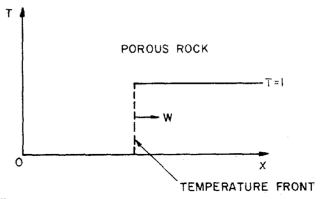
\includegraphics[width=4in]{tf1.png} 
   \caption{Thermal front moving with velocity $w$ through a porous rock}
   \label{fig:tf1}
\end{figure}
\\
Two cases can be considered. In the first case the rock and fluid properties are assumed constant. In this case equation (\ref{eq:cl3}) becomes:
\begin{equation}
\frac{\partial u}{\partial t}+\left( \frac{u_{w}}{\phi} \frac{\phi\rho_{w}c_{w}}{(1-\phi)\rho_{r}c_{r}+\phi\rho_{w}c_{w}} \right)\frac{\partial u }{\partial x} = 0
\end{equation}

By applying the method of characteristics, Stopa and Wajnarowki  \cite{Waj05}, derived the thermal front velocity $v_{TF}$:
\begin{equation}
v_{TF} =  \frac{u_{w}}{\phi} \left(\frac{\phi\rho_{w}c_{w}}{(1-\phi)\rho_{r}c_{r}+\phi\rho_{w}c_{w}} \right)
\end{equation}
In the second case the fluid and rock properties are temperature dependent. Equation (\ref{eq:cl3}) is therefore nonlinear and the method of characteristics fail to give a physical solution \cite{Waj05, Risebro07}, see Figure \ref{fig:nonp}.

\begin{figure}[H] %  figure placement: here, top, bottom, or page
   \centering
   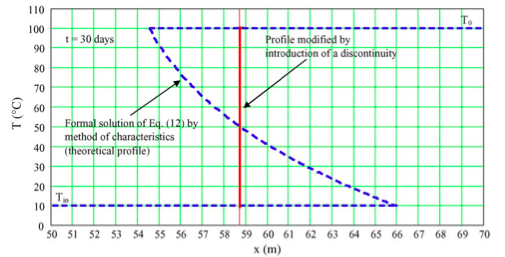
\includegraphics[width=4in]{np.png} 
   \caption{Non physical solution obtained in \cite{Waj05} from the method of characteristics}
   \label{fig:nonp}
\end{figure}

In this case The solution of equation (\ref{eq:cl3}) with initial data (\ref{eq:i}) see \cite{Waj05} is multivalued which mean that the solution is discontinuous. To obtain a physically acceptable solution, a discontinuity was inserted in the solution at position $z$ such that conservation of energy was satisfied see Figure \ref{fig:nonp}:

\begin{equation}\label{eq:cew}
t\frac{u_{w}}{\phi}\int_{u_{l}}^{u_{r}} U(u)F(u)\mathrm{d}u=z\int_{u_{l}}^{u_{r}} U(u)\mathrm{d}u
\end{equation}
setting $v_{TF}=\frac{z}{t}$ they obtained
\begin{equation}\label{eq:sw}
v_{TF} = \frac{u_{w}}{\phi}\left(   \frac{\int_{u_{l}}^{u_{r}} U(u)F(u)\mathrm{d}u   }{ \int_{u_{l}}^{u_{r}} U(u)\mathrm{d}u    }    \right) 
\end{equation}
\\
\begin{equation}\label{eq:u1}
U(u) =(1-\phi)\rho_{r}(u)(u)c_{r}(u) + \phi \rho_{w}(u)c_{w}(u).
\end{equation}
with $U(u)$ given in Figure \ref{fig:fu}. The thermal front velocity obtained by Stopa and Wajnarowski is the weighted average of the derivative of the flux function :

\begin{equation}\label{eq:G1}
G(u) = \frac{u_{w}}{\phi}\int_{0}^{u}F(x)\mathrm{d}x \implies  \frac{d G(u)}{d u}=\frac{u_{w}}{\phi}F(u)\nonumber
\end{equation}
So that (\ref{eq:sw}) ca be written as
\begin{equation}\label{eq:sw1}
v_{TF} = \left(   \frac{\int_{u_{l}}^{u_{r}} U(u)G^{\prime}(u)\mathrm{d}u   }{ \int_{u_{l}}^{u_{r}} U(u)\mathrm{d}u    }    \right) 
\end{equation}



\begin{figure}[H] %  figure placement: here, top, bottom, or page
   \centering
   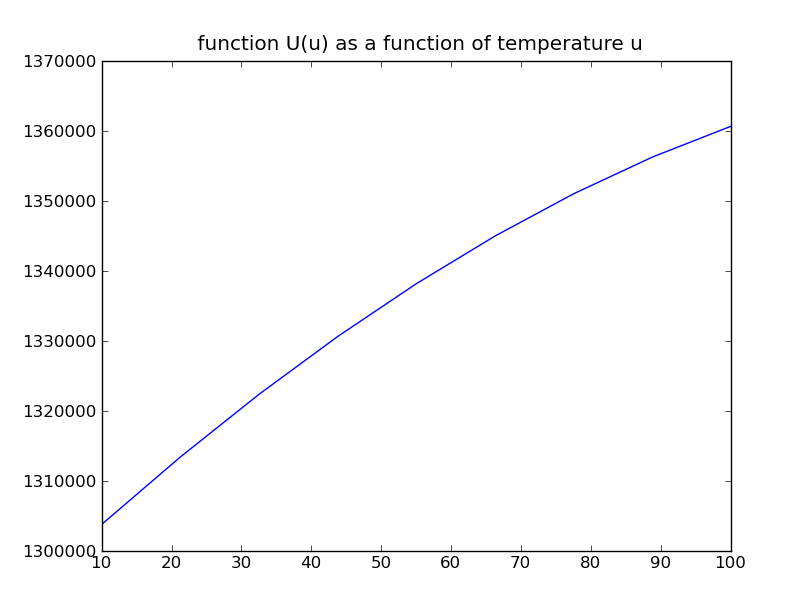
\includegraphics[width=4in]{fu.png} 
   \caption{Function $U$ given in \ref{eq:u1}}
   \label{fig:fu}
\end{figure}

%Equipped with results given in section 4.3 we are now ready to derive the thermal front velocity induced by injecting cold fluid into a hot geothermal reservoir. 

\subsection{Thermal front velocity predicted by the theory of conservation law}
Injecting colder water into a hot geothermal reservoir can be formulated as a Riemann problem : Find the unique weak solution $u$ of 
\begin{equation}\label{eq:rp}
\frac{\partial u}{\partial t} +\frac{ \partial G(u) }{\partial x}=0, \quad u(x,0)=g(x)
\end{equation}

\[ g(x) = \left\{ 
  \begin{array}{l l }
    u_{l} & \quad \text{if $x\leq 0$ }\\
    
    u_{r} & \quad \text{if $x\geq 0$ }.
  \end{array} \right.\]
satisfying the Rankine-Hugoniot shock condition and the Kruzkov entropy condition. The shock condition gives the speed $s$ of the discontinuity solution of (\ref{eq:rp}):

\begin{equation}\label{eq:rh}
s = \frac{G(u_{r})-G(u_{l})}{u_{r}-u_{l}}
\end{equation} 

The Kruzkov entropy condition:

\begin{equation}
\int_{0}^{T}\int_{-\infty}^{\infty}\left( \mid u-k \mid \varphi_{t}+q(u,k)\varphi_{x} \right) \mathrm{d}x \mathrm{d}t + \int \mid u(x,0)-k \mid \varphi(x,0) \mathrm{d}x  \geq 0 
\end{equation}
 is the extra condition satisfy by the unique solution of (\ref{eq:rp}) see \cite{Risebro07} for detail. $q(u,k)=sign(u,k)(G(u)-G(k))$, $k$ is a non negative constant and $\varphi$ is any non negative test function.\\
\\
From \cite{Risebro07}, the unique solution of (\ref{eq:rp}) satisfying the Rankine-Hugoniot condition and the Krizkov entropy condition is:


\begin{equation}
u(x,t) = \left\{
\begin{array}{rl}
u_{l} & \text{if } x \leq G^{\prime}_{\cup}(u_{l})t,\\
(G^{\prime}_{\cup})^{-1}(\frac{x}{t}) & \text{if }G^{\prime}_{\cup}(u_{l})t\leq x \leq G^{\prime}_{\cup}(u_{r})t\\
u_{r} & \text{if } x \geq G^{\prime}_{\cup}(u_{r})t
\end{array} \right.
\end{equation}
If $u_{l}<u_{r}$, and:
\begin{equation}
u(x,t) = \left\{
\begin{array}{rl}
u_{l} & \text{if } x \leq G^{\prime}_{\cap}(u_{l})t,\\
(G^{\prime}_{\cap})^{-1}(\frac{x}{t}) & \text{if }G^{\prime}_{\cap}(u_{l})t\leq x \leq G^{\prime}_{\cap}(u_{r})t\\
u_{r} & \text{if } x \geq G^{\prime}_{\cap}(u_{r})t
\end{array} \right.
\end{equation}
if $u_{l}>u_{r}$,
 where $G_{\cup},_\cap $ is the lower and the upper convex envelope of $G$ respectively.

%%%%%%%%%%%%%%%%%%%%%%%%%%%%%%%%%%%%%%%%%%%%%%%%%%%%%%%%%%%%%%%%%%%%%%%%%%%%%%%%%%%%%

%\subsection{Constant temperature rock and fluid properties}
%Assuming that the density and the heat capacity of rock and fluid are constant,  (\ref{eq:rp}) becomes
%
%\begin{equation}\label{eq:rpc}
% u_{t} +Fu_{x}=0, \quad u(x,0)=g(x)
%\end{equation}
%
%\[ g(x) = \left\{ 
%  \begin{array}{l l }
%    u_{l} & \quad \text{if $x\leq 0$ }\\
%    
%    u_{r} & \quad \text{if $x\geq 0$ }.
%  \end{array} \right.\]
%
%with 
%
%\begin{equation}\label{eq:Fc}
%F=\frac{   \phi \rho_{w} c_{w}     }{  (1-\phi)\rho_{r} c_{r} +  \phi \rho_{w}c_{w}     }
%\end{equation}
%
%We assume that the injected temperature $u_{l}$ is less then the reservoir temperature $u_{r}$. The unique solution $u$ is a shock moving at the speed $s$
%\[ u(x,t) = \left\{ 
%  \begin{array}{l l }
%    u_{l} & \quad \text{if $x\leq st$ }\\
%    
%    u_{r} & \quad \text{if $x\geq st$ }.
%  \end{array} \right.\]
%
%with $s$ given by the Rankine-Hugoniot shock condition 
%
%\begin{equation}
%\begin{aligned}
%s&=V_{w}\frac{G(u_{l})-G(u_{r})}{u_{l}-u_{r}}\\
%  &=\frac{Fu_{l}-Fu_{r}}{u_{l}-u_{r}}\\
%  &=F
%\end{aligned}
%\end{equation}
%
%Physically, a shock wave is a disturbance that induce abrupt change in the physical characteristic of the medium though which its propagates. When cold water is injected into the hot reservoir, at the interface between the cold water movement and the hot reservoir they is an abrupt change in temperature. This interface moves at the speed equal to $s$:
%\begin{equation}\label{eq:Fc}
%V_{TF}=s=V_{w}\frac{   \phi \rho_{w} c_{w}     }{  (1-\phi)\rho_{r} c_{r} +  \phi \rho_{w}c_{w}     }
%\end{equation}
%which is the cold front velocity.
%This result is the same as the one obtained by Bodvarsson \cite{Bod-R72} and Stoppa and Wajnarowski \cite{Waj05}, using the characteristics method. We should however note that the characteristics method fail to provide physically acceptable solution when the fluid and rock properties are temperature dependent \cite{Evan00}, \cite{Waj05}.
%
%%%%%%%%%%%%%%%%%%%%%%%%%%%%%%%%%%%%%%%%%%%%%%%%%%%%%%%%%%%%%%%%%%%%%%%%%%%%%%%%%%%
When fluid and rock properties depend continuously on temperature, The flux function $G$ is given by 
\begin{equation}
G(u) = V_{w}\int_{0}^{u} F(\theta)\mathrm{d}\theta\nonumber
\end{equation}

with 

\begin{equation}\label{eq:FF}
F(u)=\frac{  \phi \rho_{w}(u)\left(  \frac{\partial (c_{w}(u) u)  }{\partial u  }   \right)    }{  (1-\phi)\left( \frac{ \partial (\rho_{r}(u)  c_{r}(u) u) }{\partial u}\right) +  \phi \rho_{w}(u)\left(  \frac{\partial (c_{w}(u)u)  }{\partial u  } \right)     }
\end{equation}

\begin{figure}[H] %  figure placement: here, top, bottom, or page
   \centering
   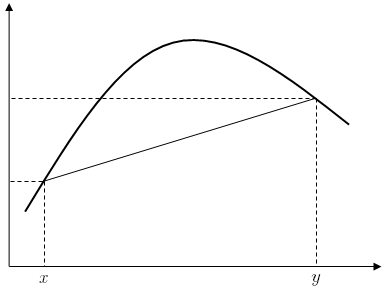
\includegraphics[width=2.7in]{G.png} 
      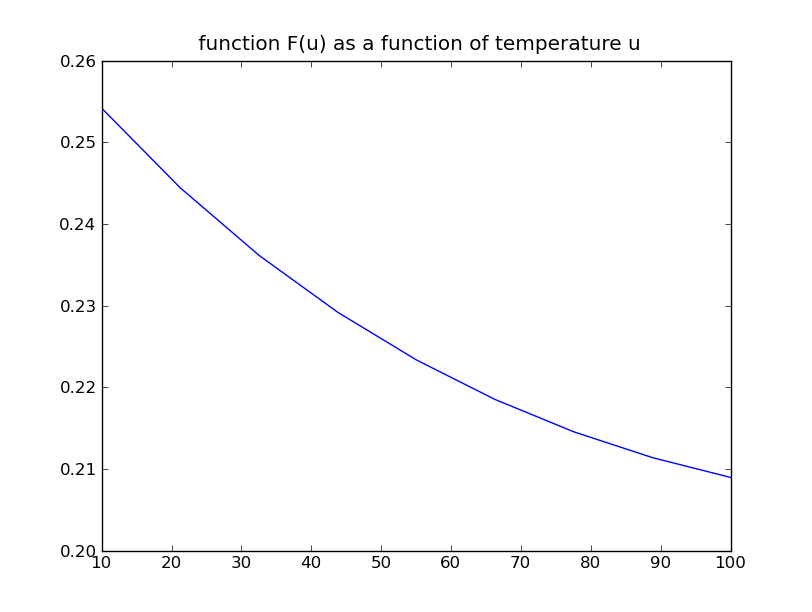
\includegraphics[width=2.7in]{F.png} 
   \caption{Function $F$ and $G$ with temperature $(x=u_{l}, y=u_{r})$}
   \label{fig:fg}
\end{figure}

From figure \ref{fig:fg} $F$ is monotonically decreasing on $[u_{l}=10,u_{r}=100]$, therefore the flux function $G$ is concave on that interval. The lower convex envelope $G_{\cup}$ of $G$  is the line passing through the points $(u_{l},G(u_{l}))$ and $(u_{r},G(u_{r}))$. In this case the unique solution of (\ref{eq:rp}) moving at the speed $s=V_{TF}$ is given by 

\[ u(x,t) = \left\{ 
  \begin{array}{l l }
    u_{l} & \quad \text{if $x\leq st$ }\\
    
    u_{r} & \quad \text{if $x\geq st$ }.
  \end{array} \right.\]
  
  \begin{figure}[htbp] %  figure placement: here, top, bottom, or page
     \centering
     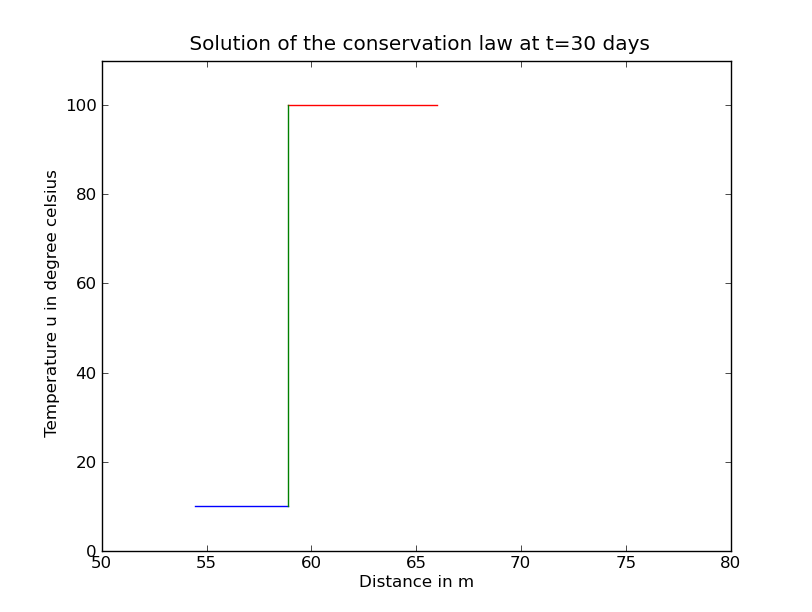
\includegraphics[width=4in]{u0.png} 
     \caption{Solution of \ref{eq:rp} at $t$ = 30 days}
     \label{fig:u0}
  \end{figure}
  with 
  $s=V_{TF}$ given by the Rankine-Hugoniot shock condition
  \begin{align}\label{eq:si}
s &=v_{TF} \nonumber \\
   &=\frac{  G(u_{l})-G(u_{r})   }{ u_{l}-u_{r} } \nonumber \\
  &=\frac{\frac{u_{w}}{\phi}}{(u_{r}-u_{l})}\left( \int_{0}^{u_{r}} F(u)\mathrm{d}u  - \int_{0}^{u_{l}} F(u)\mathrm{d}u \right)\nonumber \\
  &=\frac{\frac{u_{w}}{\phi}}{(u_{r}-u_{l})}\left( \int_{0}^{u_{l}} F(u)\mathrm{d}u +\int_{u_{l}}^{u_{r}} F(u)\mathrm{d}u   - \int_{0}^{u_{l}} F(u)\mathrm{d}u \right)\nonumber \\
  &=\frac{1}{(u_{r}-u_{l})}\left( \int_{u_{l}}^{u_{r}} \frac{u_{w}}{\phi}F(u)\mathrm{d}u   \right) 
\end{align}

\subsection{Numerical values and discussion}
In this section we compared numerically the values of the thermal front velocity from \cite{Waj05} and the theory of conservation laws. 
%Recall that the thermal front velocity $V_{TF}$ given in (\ref{eq:si}) differ from the one obtained in \cite{Waj05} in it expression. In the later, the method of characteristic was applied, resulting in a nonphysical solution. (see figure \ref{fig:np}). To obtain a physically acceptable solution, a discontinuity was inserted in the solution at position $z$ such that conservation of energy was satisfy:
%
%\begin{equation}\label{eq:cew}
%tv_{w}\int_{u_{l}}^{u_{r}} U(u)F(u)\mathrm{d}u=z\int_{u_{l}}^{u_{r}} U(u)\mathrm{d}u
%\end{equation}
%setting $v_{TF}=\frac{z}{t}$ they obtained
%\begin{equation}\label{eq:sw}
%v_{TF} = v_{w}\left(   \frac{\int_{u_{l}}^{u_{r}} U(u)F(u)\mathrm{d}u   }{ \int_{u_{l}}^{u_{r}} U(u)\mathrm{d}u    }    \right) 
%\end{equation}
%\\
%\begin{equation}\label{eq:u1}
%U(u) =(1-\phi)\rho_{r}(u)(u)c_{r}(u) + \phi \rho_{w}(u)c_{w}(u).
%\end{equation}
%with $U(u)$ given in Figure \ref{fig:fu}.
%
%\begin{figure}[H] %  figure placement: here, top, bottom, or page
%   \centering
%   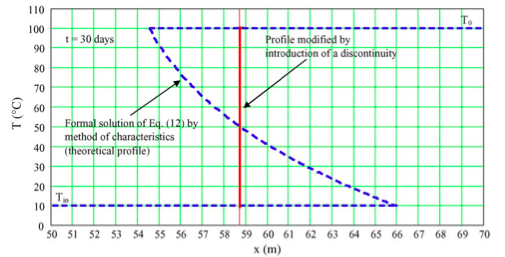
\includegraphics[width=4in]{np.png} 
%   \caption{Non physical solution obtained in \cite{Waj05} from the method of characteristics}
%   \label{fig:np}
%\end{figure}
%
%\begin{figure}[H] %  figure placement: here, top, bottom, or page
%   \centering
%   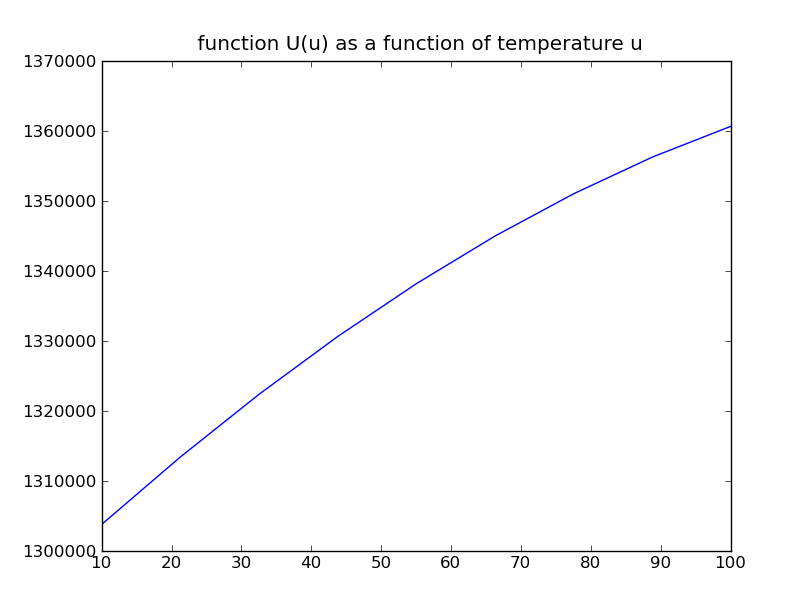
\includegraphics[width=4in]{fu.png} 
%   \caption{Function $U$ given in \ref{eq:u1}}
%   \label{fig:fu}
%\end{figure}


%%%%%%%%%%%%%%%%%%%%%%%%%%%%%%%%%%%%%%%%%%%%%%%%%%%%%%%%%%%%%%%%%%%%%%%%%%%%%%%%%%%
%\subsection{Numerical result}
%The trapezoidal rule from calculus state that the integral of a function $f$ on an interval $[a,b]$ can be approximated  by
%\\
%\begin{equation}\label{eq:trap}
%\int_{a}^{b}f(x) \mathrm{d}x \approx\frac{b-a}{2n}\left( f(a)+f(b)+\sum_{i=1}^{n-1}f(a+ih)\right)
%\end{equation}
%\\
%with absolute and asymptotic error (computable error) given respectively by
%
%\begin{equation}\label{eq:a}
%E_{n}^{a}=-\frac{h^{2}(b-a)}{12}(f^{\prime\prime}(c_{n}))
%\end{equation}
%and 
%
%\begin{equation}\label{eq:c}
%E_{n}^{c}=-\frac{h^{2}}{12}(f^{\prime}(b)-f^{\prime}(a))
%\end{equation}
%\\
%with some unknown $ c_{n} \in[a,b]$ and $ h = \frac{b-a}{n}$. Equation (\ref{eq:c}) is also called upper bound error and can also be written in terms of $n$ as 
%\\
%\begin{equation}\label{eq:cc}
%E_{n}^{c}=\frac{c}{n^{2}}
%\end{equation}
%with 
%
%\begin{equation}
%c=-\frac{(b-a)}{12}(f^{\prime}(b)-f^{\prime}(a)).\nonumber
%\end{equation}
%\\
%To evaluate the derivative of $f$ we use the finite difference approximation 
%\\
%\begin{equation}
%f^{\prime}(x)\approx \frac{f(x+h)-f(x-h)}{2h} \nonumber
%\end{equation}
%\\
%with approximation error given by
%\\
%\begin{equation}
%Err = \frac{1}{6}f^{\prime\prime\prime}h^{2}+O(h^{3}) = O(h^{2}).\nonumber
%\end{equation}
%
%
%
%
%
\begin{table}[H]
	\begin{center}
		\begin{tabular}{|l|c|c|c|r|}
		\hline
			$u_{l}$ & $u_{r}$ & [$V_{TF}$ from (\ref{eq:si}) ,$10^{-5}m/s$]& [$v_{TF}$ for (\ref{eq:sw}), $10^{-5}m/s$ ]&[$V_{TF}-v_{TF}$]  \\ \hline
			10 & 100 & $2.261$ & $2.257$  & $4*10^{-8}$   \\ 
			55 & 100 & $2.15$  & $2.15$       & $0.0  $    \\ 
			10 & 55 & $2.370$   & $2.369$    & $10^{-8}$  \\ 
			20 & 80 & $2.271$    & $2.269$  & $2*10^{-8} $ \\ 
			30 & 70 & $2.264$    & $2.263$    & $10^{-8} $ \\ 
			40 & 60 & $2.260$       &  $2.259$  & $10^{-8} $\\
			\hline
		\end{tabular}
		\caption{approximated values for evaluating (\ref{eq:si}) and (\ref{eq:sw})}
		\label{tab:ap}
	\end{center}
\end{table}
The thermal front velocity predicted by the theory of conservation laws is slimly higher than the one obtained by Stopa and Wajnaroski in \cite{Waj05}. A relative error of $10^{-3}$ is observed between the two results. 



%For symmetric and spherical flow problem, Bodvarsson presented a method to compute the radius of propagation of the thermal front velocity. Assume that a mass $M = Qt$ of fluid at time $t$ with temperature $u_{l}$ is injected at a flow rate $Q$ in a volume $V$ of reservoir rock with temperature $u_{r}$. If q is the magnitude of the mass flow vector of the fluid From \cite{Bod-R72}
%%we have the following relation
%\begin{equation}
%\frac{V}{Qt} = \frac{V_{TF}}{q} 
%\end{equation}
%
%For spherical symmetric flow the radius of propagation is 
%\begin{equation}
%r = \left(  \frac{3V_{TF}Qt}{4\pi q}         \right)^{\frac{1}{3}}
%\end{equation}
%and for cylindrical flow the radius of propagation is
%\begin{equation}
%r = \left(  \frac{V_{TF}Qt}{\pi q}         \right)^{\frac{1}{2}}
%\end{equation}
%
%\begin{figure}[htbp] %  figure placement: here, top, bottom, or page
%   \centering
%   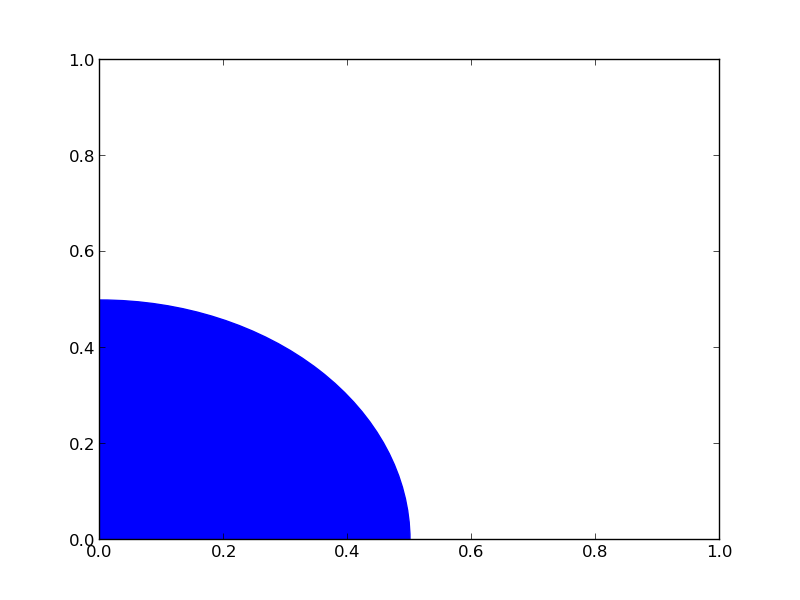
\includegraphics[width=2.5in]{waj.png}
%      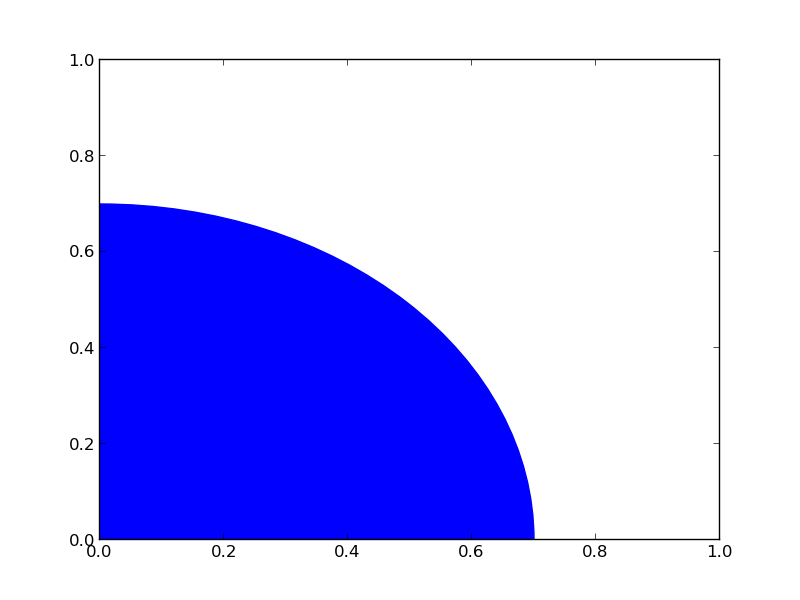
\includegraphics[width=2.5in]{cl.png} 
% 
%   \caption{Illustration of the radius of propagation for thermal front velocity from \ref{eq:sw} and \ref{eq:si}}
%   \label{fig:example}
%\end{figure}
%The radius of cold water propagation is therefore proportional to the thermal front velocity for spherical and cylindrical symmetric flow.
%
%\begin{table}[H]
%	\begin{center}
%		\begin{tabular}{|l|c|r|}
%		\hline
%			$n$ & Error for equation (\ref{eq:si}) & error for equation (\ref{eq:sw}) \\ \hline
%			10 & $5.6*10^{-5}$ & $174.6$ \\ 
%			40 & $4*10^{-6}$ & $10.9$ \\ 
%			70 & $10^{-6}$ & $3.5$ \\ 
%			107 & $0.0$ & $1.5$ \\ 
%			$10^{5}$ & $0.0$ & $1.2*10^{-5}$\\
%		\hline
%		\end{tabular}
%		\caption{Convergence test for the trapezoidal rule (\ref{eq:trap}) for equation (\ref{eq:si}) and (\ref{eq:sw})}
%		\label{tab:trapc}
%	\end{center}
%\end{table}
%
%
%Table \ref{tab:ap} shows that the values obtained by using either equation (\ref{eq:sw}) or (\ref{eq:si}) are equal within an error of $10^{-8}$. Table \ref{tab:trapc} indicates that the error in evaluating the integral in (\ref{eq:si}) converge to zero from $n=107$, while the error in evaluating the lower integral in equation (\ref{eq:si}) does not converge. To have convergence we are force to use a more accurate integration scheme such as Simpson (1/3) rule which is fourth order accurate. Using Simpson rule, the integral of a function $f$ is approximated by
%\\
%\begin{equation}\label{eq:sim}
%\int_{a}^{b}f(x) \mathrm{d}x \approx\frac{b-a}{3n}\left( f(a)+f(b)+4\sum_{i=1(odd)}^{n-1}f(a+ih)+ 2\sum_{i=2(even)}^{n-2}f(a+ih)\right)
%\end{equation}
%\\
%with computed or upper bound error given by
%\\
%\begin{equation}\label{eq:errs}
%E^{c}_{n} = -\frac{h^{4}}{180}(f^{\prime\prime\prime}(b)-f^{\prime\prime\prime}(a)).
%\end{equation}
%\\
%The third derivative of $f$ can be approximated by finite difference as 
%\\
%\begin{equation}
%f^{\prime}(x)\approx \frac{-\frac{1}{2} f(x-2h)+f(x-h)-f(x+h)+\frac{1}{2}f(x+2h)}{h^{3}} \nonumber
%\end{equation}
%\\
%
%\begin{table}[H]
%	\begin{center}
%		\begin{tabular}{|l|c|r|}
%		\hline
%			$n$ & Error for equation (\ref{eq:si}) & error for equation (\ref{eq:sw}) \\ \hline
%			10 & $5.6*10^{-5}$ & $72975$ \\ 
%			50 & $4*10^{-6}$ & $116.76$ \\ 
%			176 & $0.0$ & $0.76$ \\ 
%			6000 & $0.0$ & $10^{-6}$ \\ 
%			$6181$ & $0.0$ & $0.0$\\
%		\hline
%		\end{tabular}
%		\caption{Convergence test for Simpson (1/3) rule (\ref{eq:sim}) for equation (\ref{eq:si}) and (\ref{eq:sw})}
%		\label{tab:sim}
%	\end{center}
%\end{table}
%
%
%\begin{table}[H]
%	\begin{center}
%		\begin{tabular}{|l|c|c|c|r|}
%		\hline
%			a & b & [$V_{TF}$ from (\ref{eq:si}) ,$10^{-5}m/s$]& [$v_{TF}$ for (\ref{eq:sw}), $10^{-5}m/s$ ]&[$V_{TF}-v_{TF}$]  \\ \hline
%			10 & 100 & $2.261$ & $2.257$  & $4*10^{-8}$   \\ 
%			55 & 100 & $2.15$  & $2.15$       & $0.0  $    \\ 
%			10 & 55 & $2.370$   & $2.369$    & $10^{-8}$  \\ 
%			20 & 80 & $2.271$    & $2.269$  & $2*10^{-8} $ \\ 
%			30 & 70 & $2.264$    & $2.263$    & $10^{-8} $ \\ 
%			40 & 60 & $2.260$       &  $2.260$  & $0.0 $\\
%			\hline
%		\end{tabular}
%		\caption{approximated values for evaluating (\ref{eq:si}) and (\ref{eq:sw}) using (\ref{eq:sim})}
%		\label{tab:aps}
%	\end{center}
%\end{table}
%
%\begin{table}[H]
%	\begin{center}
%		\begin{tabular}{|lc|c|c|r|}
%		\hline
%			n& $E_{1}$ ($10^{-6}$) &$E_{2}$&$E_{3}$ &convergence rate  \\ \hline
%			4 & $351$& $663.35$ & $469.2$   & $(E_{1})$: $[1.99,2.01,1.98]$   \\ 
%			5& $225$ & $425.5$  & $300.31$  & $(E_{2})$: $[2.00,1.99,2.02]   $    \\ 
%			6 & $156$ & $294.8$   & $208.5$   & $(E_{3})$: $[1.99,2.00,1.99] $  \\ 
%			7 & $115$ & $216$    & $153.2$  & \\
%			
%			\hline
%		\end{tabular}
%		\caption{Convergence rate for the error in the trapezoidal rule}
%		\label{tab:apr}
%	\end{center}
%\end{table}
%
%
%In Table \ref{tab:apr} $E_{1}$ represent the upper bound error in evaluating \ref{eq:si}, $E_{2}$ represent the upper bound error in evaluating the upper integral of \ref{eq:sw} and $E_{3}$ the upper bound error in evaluating the lower integral. The rate of convergence is bout 2, which is the same as the error for the trapezoidal rule. This shows that the numerical results obtained using the trapezoidal rule are accurate.\\ 
%Table \ref{tab:aps} shows the result obtained using Simpson $(1/3)$ rule. This result is similar to the one obtained in table \ref{tab:ap} except in the last entry of the tables. The largest difference between the result obtained from \cite{Waj05} and the theory of conservation laws is an order of $10^{-8}$. 

%\section{discussion}
%For temperature dependent fluid and rock properties, the mass and energy equation for fluid flow in porous medium can be reduced to a conservation laws when heat conduction is neglected. In this case, injecting colder water into a hot geothermal reservoir can be solve as a Riemann problem  for the conservation laws. The thermal front velocity coincide with the velocity of the discontinuity solution satisfying the Kruzkov entropy solution \cite{Risebro07}. Our result was compared with the result obtained in \cite{Waj05}. in the later, starting with a nonphysical solution, a discontinuity was inserted into the solution such that the new physical acceptable solution satisfies the conservation of energy entropy condition.                  
%A numerical simulation showed that the error in evaluating the thermal front velocity from our result goes rapidly to zero compared with the error in evaluating the thermal front velocity obtained in \cite{Waj05}.

%Thermal front or cold injected front is the interface between the cold injected fluid and the hot reservoir. At this interface, temperature changes very rapidly between injected fluid temperature and reservoir temperature. To capture this mathematically, a jump discontinuity is inserted at this interface. As cold water flows through the reservoir, the jump discontinuity position moves as well. Its position at any time gives the position of the cold moving front. \\
%Our computed thermal front velocity agrees with the one obtained in \cite{Bod-R72} for temperature independent rock and fluid properties event though different method were used. For temperature dependent fluid and rock properties, Our result and the one in \cite{Waj05} were numerically closed. However our method is based on a well established theory of hyperbolic conservation laws described in \cite{Risebro07}. The Riemann problem upon which we derived the thermal front velocity is well posed \cite{Risebro07}.\\ 
%A numerical solution of the conservation laws using a stabilised numerical scheme for conservation laws, could be used to simulate cold front propagation to further this work.
%This work could also be extended to the case where hot water is injected to a colder reservoir.  


 
% Chapter 3

\chapter{Lumped parameters modelling in Munadarnes geothermal system } % Main chapter title

\label{Chapter3} % For referencing the chapter elsewhere, use \ref{Chapter1} 

\lhead{Chapter 3. \emph{Lumped parameter modelling with case study}} % This is for the header on each page - perhaps a shortened title

%----------------------------------------------------------------------------------------


%----------------------------------------------------------------------------------------
\section{Munardanes low temperature system}

\begin{figure}[H] %  figure placement: here, top, bottom, or page
   \centering
   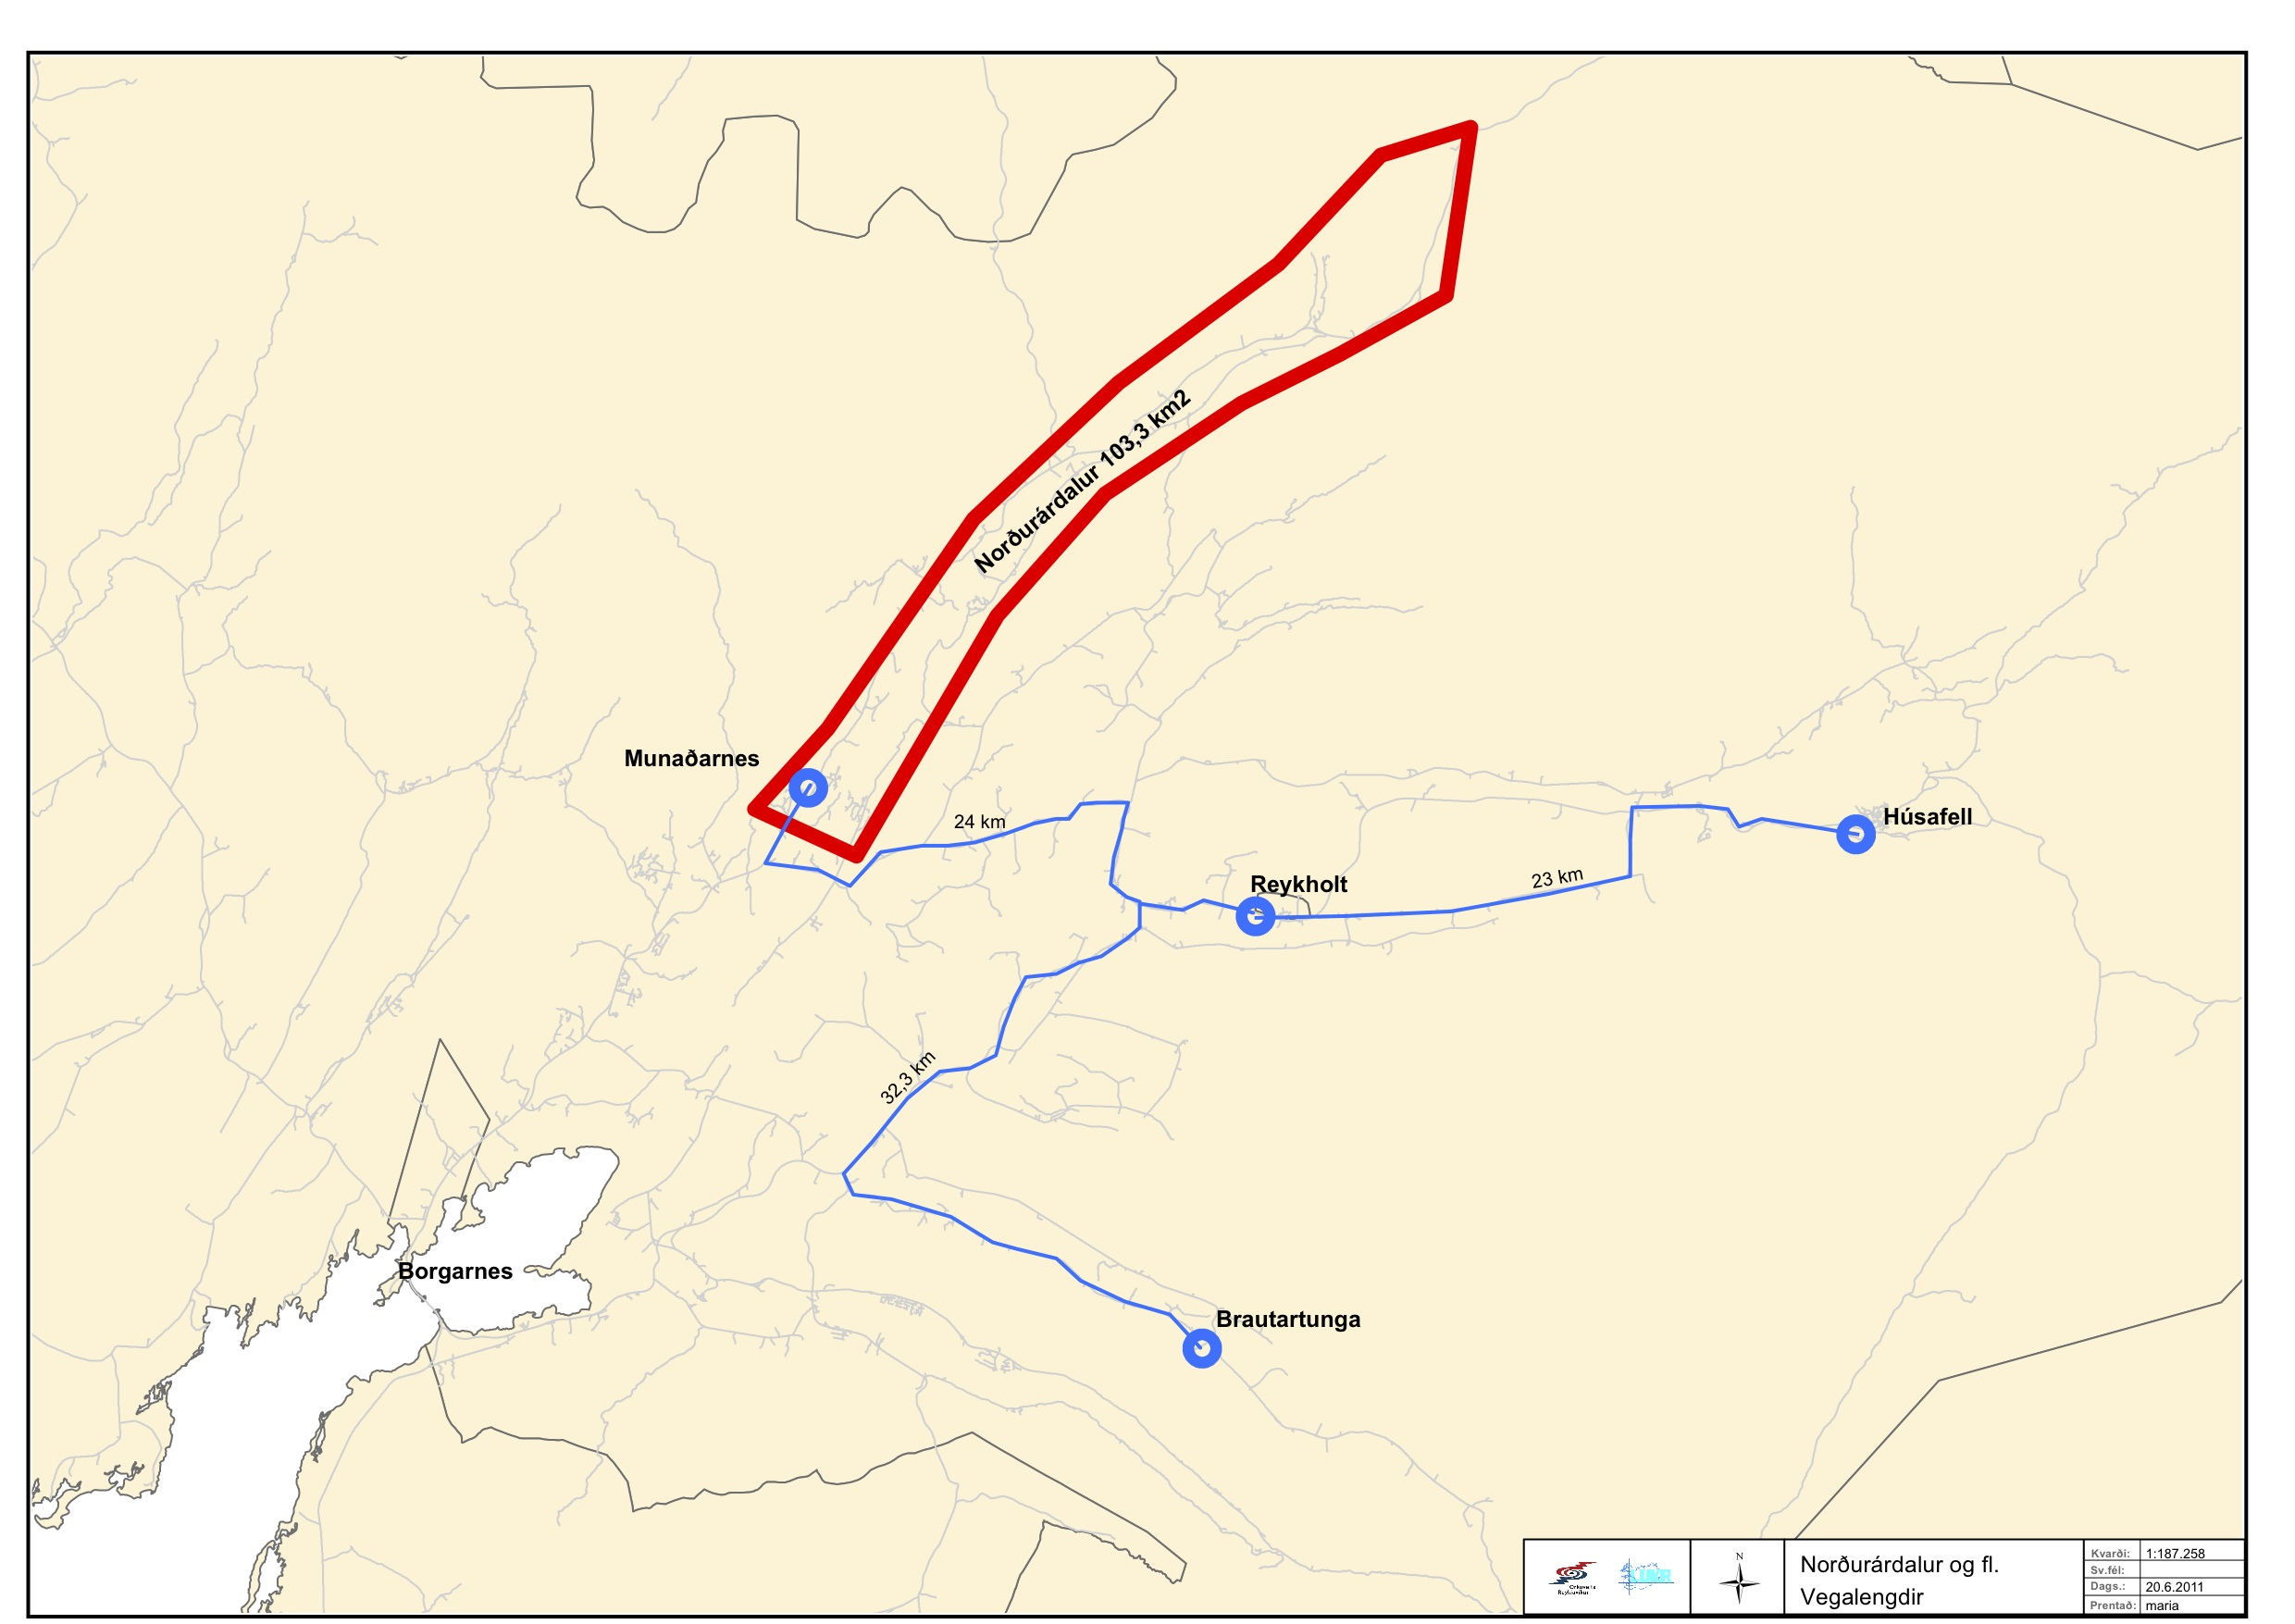
\includegraphics[width=5in]{nordu.jpg} 
   \caption{ Borgarfjordur thermal field and Nordurardalur thermal system}
   \label{fig:nordu}
\end{figure}
The Munardanes reservoir is situated in the Nordurardalur geothermal field. The later is located in west Iceland in the Borgarfjordur thermal field situated in the Borgarfjordur region. The Borgarfjordur thermal field is the largest low temperature geothermal field in Iceland. It comprises known thermal systems such as the Reykholt thermal system, the Bear thermal system, the Brautartunga thermal system, England thermal system, and the Husafell thermal system (Johannesson et al. 1980, Gunnlaugsson 1980). The natural discharge of the Borgarfjordur thermal system also called the Reykholtsdalur thermal system is estimated to 450$l/s$ of boiling water (Georgsson et al. 1984).  Within the Borgarfjordur thermal field, the Reykholf thermal system is by fare the largest thermal system with a total discharge of 400$l/s$ (Georgsson et al. 1980). The Nordurardalur thermal system is located north-west to the five major thermals systems mention above. It is a N-W long band of about 103 $km^{2}$ .

\subsection{Geological setting}
\begin{figure}[H] %  figure placement: here, top, bottom, or page
   \centering
   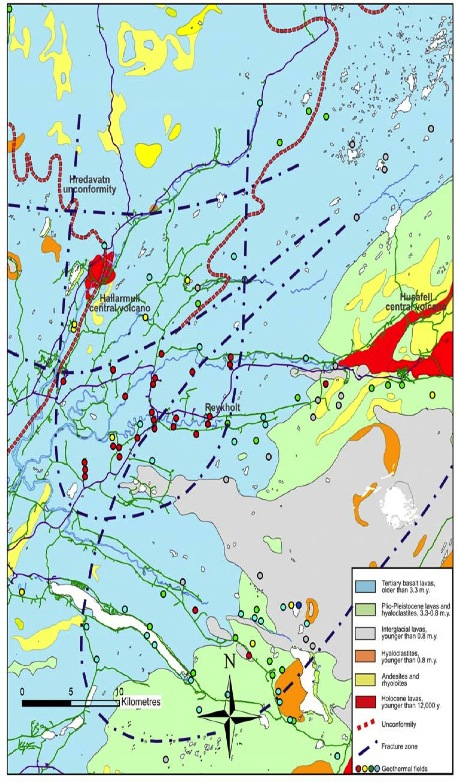
\includegraphics[width=4in]{bgeo.jpg} 
   \caption{Geological map of Borgarfjordur thermal field}
   \label{fig:bgeo}
\end{figure}

Upper tertiary ($>$3.3 Myr) basaltic lava flow constitute the basement of the Borgarfjordur region. This lava flow is characterised by a uniform lithology, either uniform texture or composition. The oldest rock being 14-15 Myrs. The bulk of this tertiary lava flow is made of tholeiites basaltic rock separated by minor clastic interbeds (Saemundsson, 1979). The tholeiites basaltic lava pile is characterized by its content in sodium which is less than other basaltic rock. The Borgarfjordur thermal field is bounded from the east by the western volcanic rift zone and the snaefellnes volcanic zone from the west. The later present little or no rifting. Those two volcanic zones represent the origin of the tertiary lava flow.  However, the tholeiites content of the lava flow suggest that the lava flow is predominantly from the Sneafellsnes volcanic flank zone. \\
\\
 Both unconformity and anticline structures are visible in the region. The later formed from rift relocation (Saemundsson, 1967). Recall that an anticline is defined as layers of sedimentary rock having the oldest strata in its core and forming a convex shape. An unconformity is a planar structure indicating a discontinuity in a geologicale structure due to erosive forces. The anticline axis is defined as the line of intersection of the perpendicular plane cutting the anticline in two symmetric parts. The Borganes anticline runs NE-SW (saemundsson, 1977). The lava flow dip towards the Reykjanes-Langjokull rift zone to the east of the anticline axis. The Hredavatn unconformity is situated in north of Hredavatn lake. This unconformity indicate intense erosive forces acting in the borgarfjordur region.

\subsection{Geophysical and hydrological setting}

The geophysics of the region is characterised by the volcanism, the tectonic and the different forces affecting the earth crustal structure. The region is located between the Sneafellsnes volcanic flank and the Reykjanes-Langjokull volcanic rift. The later is made of the Reykjanes peninsula and the Western volcanic zone. The Reykjanes-Lanjokull rift is characterised by faulting resulting from tensional stress in the earth crust.  The Nordurardalur geothermal system is confined within the WNW-ESE, N-S  fractures zone   and between the Hradavatn unconformity and the Borganes anticline. An extinct central volcano is sitting within the Nordurardalur thermal system.\\
The resistivity in Nordurardalur alternate between 20 and 100 $\Omega m$.  The 20 $\Omega m$ resistivity part is located in the lowest part of the Nordurardalur band and quickly 
increase to 60 and 100 as we move North east. The value alternate to 30-40 then decrease to 20 before increasing to about 30 $\Omega m$.\\
\\
The geothermal water is of meteoric origin which as fallen as precipitation on the highland. The water percolate through fractures cracks or others pathways through the earth and is heated by regional heat flow. The flow pattern can be infer base on preview studies done in the main thermal systems in Borgafjordur. The Northeasterly faults are the main channels for the Nordurardalur thermal system and the seismicity in the region allows fractures to serve as flow path. The recharge zone is the Arnarvatnsheidi highland and the flow pattern is 

\subsection{Proposed conceptual model of Borgarfjordur thermal filed}
\begin{figure}[H] %  figure placement: here, top, bottom, or page
   \centering
   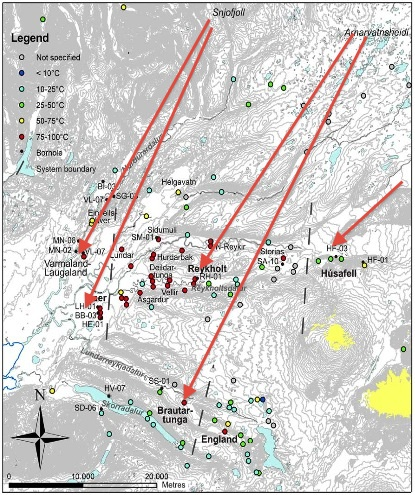
\includegraphics[width=5in]{flowp.jpg} 
   \caption{Production well in Borgarfjordur thermal field with flow patterns of the main thermal systems}
   \label{fig:flowp}
\end{figure}
Figure (\ref{fig:flowp}) indicates the flow patterns of the main thermal system in Borgarfjordur thermal field. The Reykholt and the Brautartungar thermal field recharge zone is located in the Arnarvatnsheidi high land. The Husafell thermal system recharge zone is located east to the Arnarvatnsheidi high land. For those tree systems, the easterly and north easterly faults and fractures allows the meteoric water to percolate at depth, acting as flow channels. The Nordurardalur system can be seen as a part of the Bear thermal system. The recharge zone is situated in the surrounding  of Snjofjoll, latitude 64 Degree 59 $mn$ $N$, longitude 21 Degree 11 $mn$ W. The $NS$ fractures act as flow channels, where the water flows by the Hallarmuli extinct central volcanoes. \\
\\
Heat is transfer by conduction through the earth crust from the Snaefellsnes volcanic flank and the Reykjaness-Langjokull volcanic rift zone. Heat is convected by the hot water though the fracture and fault systems at depth. The integrity of the fracture/fault system are maintain by the seismicity in the region. They also act as barriers zone. The salinity of water is the highest in the Bear thermal system as well as in the Nordurardalur system. As we move away from the Bear system the salinity decreases, being the lowest in Husafell thermal system.


%%%%%%%%%%%%%%%%%%%%%%%%%%%%%%%%%%%%%%%%%%%%%%%%%%%%%%%%


\section{Lumped parameter modelling }
Lumped parameter modelling is a cost effective high precision modelling approach for geothermal systems. It is used to simulate water level or pressure change due to production in a geothermal reservoir. By using a nonlinear iterative least square technique, the computer program LUMPFIT fit automatically the analytical response functions of lumped model to the measured data (water level or pressure), \cite{Ax-Simul-Lump89}. In the lumped model, the geothermal system is represented by tanks, characterised by storage coefficient $\kappa$ and conductor $\sigma$, simulating respectively the  storativity $s$ and permeability $K$. In this modelling process the reservoir is divided into three parts if necessary. For two dimensional flow as in this work, the fluid turbulence coefficient is neglected.

\begin{figure}[htbp] %  figure placement: here, top, bottom, or page
   \centering
   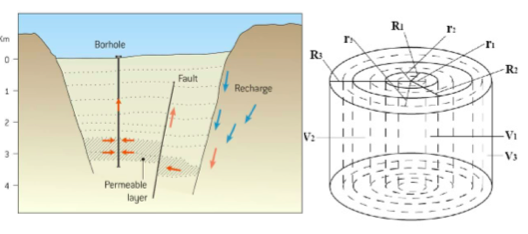
\includegraphics[width=6in]{lump1.png} 
   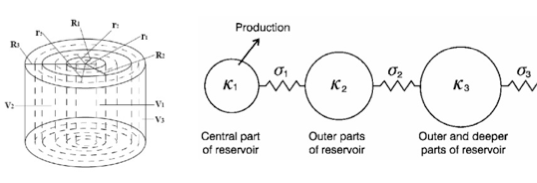
\includegraphics[width=6in]{lump0.png} 
   \caption{Subdivision of the reservoir in recharge, intermediary, and production parts}
   \label{fig:lump1}
\end{figure}

Each part is approximated by a cylindrical tanks with defined radius. The inner cylinder (inner tank) is the production part which is intersected by the production well. Adjacent to inner cylinder is an intermediaries cylinder defining the interface between the recharge part (outer cylinder) and the production part (inner cylinder).  Each cylinder are then approximated by lumped capacitors characterised by the coefficients $\kappa$ and $\sigma$ simulating  storativity $s$ and permeability at the boundary of the cylinder (capacitor).\\
\\
\\
\clearpage
The goal is to fit the theoretical  pressure response

\begin{equation}\label{eq:c}
 P(t)=�\sum Q\frac{A_{i}}{L_{i}}(1-exp(-L_{i}t))+QBt 
\end{equation}

\begin{equation}\label{eq:o}
 P(t)=�\sum Q\frac{A_{i}}{L_{i}}(1-exp(-L_{i}t)) 
\end{equation}
to a set of measured water level data, for an open system and a closed system respectively. Recall that a geothermal system is open when sufficient fluid flow through it boundaries to allow recharge. The opposite is true for a closed system.

The parameters  $A_{i}, L_{i}$, $B$, are function of $\kappa_{i}$ and $\sigma_{i}$.  After evaluating the unknown parameter ( $A_{i}, L_{i}$, $B$,$\kappa_{i}$ and $\sigma_{i}$ ), equations (\ref{eq:c}, \ref{eq:o}) can be used to simulate and predict water level change in time. The size $A$, the depth $H$, the approximate permeability $K$, the storativity $s$ and the  recharge mechanism of the reservoir can also be evaluated and understood using
\begin{equation}
\kappa_{i}=V_{i}s=A_{i}Hs \\
\end{equation}

\begin{equation}
K=\sigma_{i}\frac{ln(r_{i+1}/r_{i})\nu}{2\pi H}\\
\end{equation}

\begin{equation}
r_{1}=R_{1}/2, \quad r_{2}=R_{1}+(R_{2}-R_{1})/2, \quad r_{3}=R_{2}+(R_{3}-R_{2})/2\\
\end{equation}

\begin{equation}
R_{1}=\sqrt{V_{1}/\pi H}, \quad R_{1}=\sqrt{(V_{1}+V_{2})/\pi H}, \quad R_{1}=\sqrt{(V_{1}+V_{2}+V_{3})/\pi H}\\
\end{equation}

%\section{Case study: Munardanes reservoir in west Iceland}
%
%\begin{figure}[htbp] %  figure placement: here, top, bottom, or page
%   \centering
%   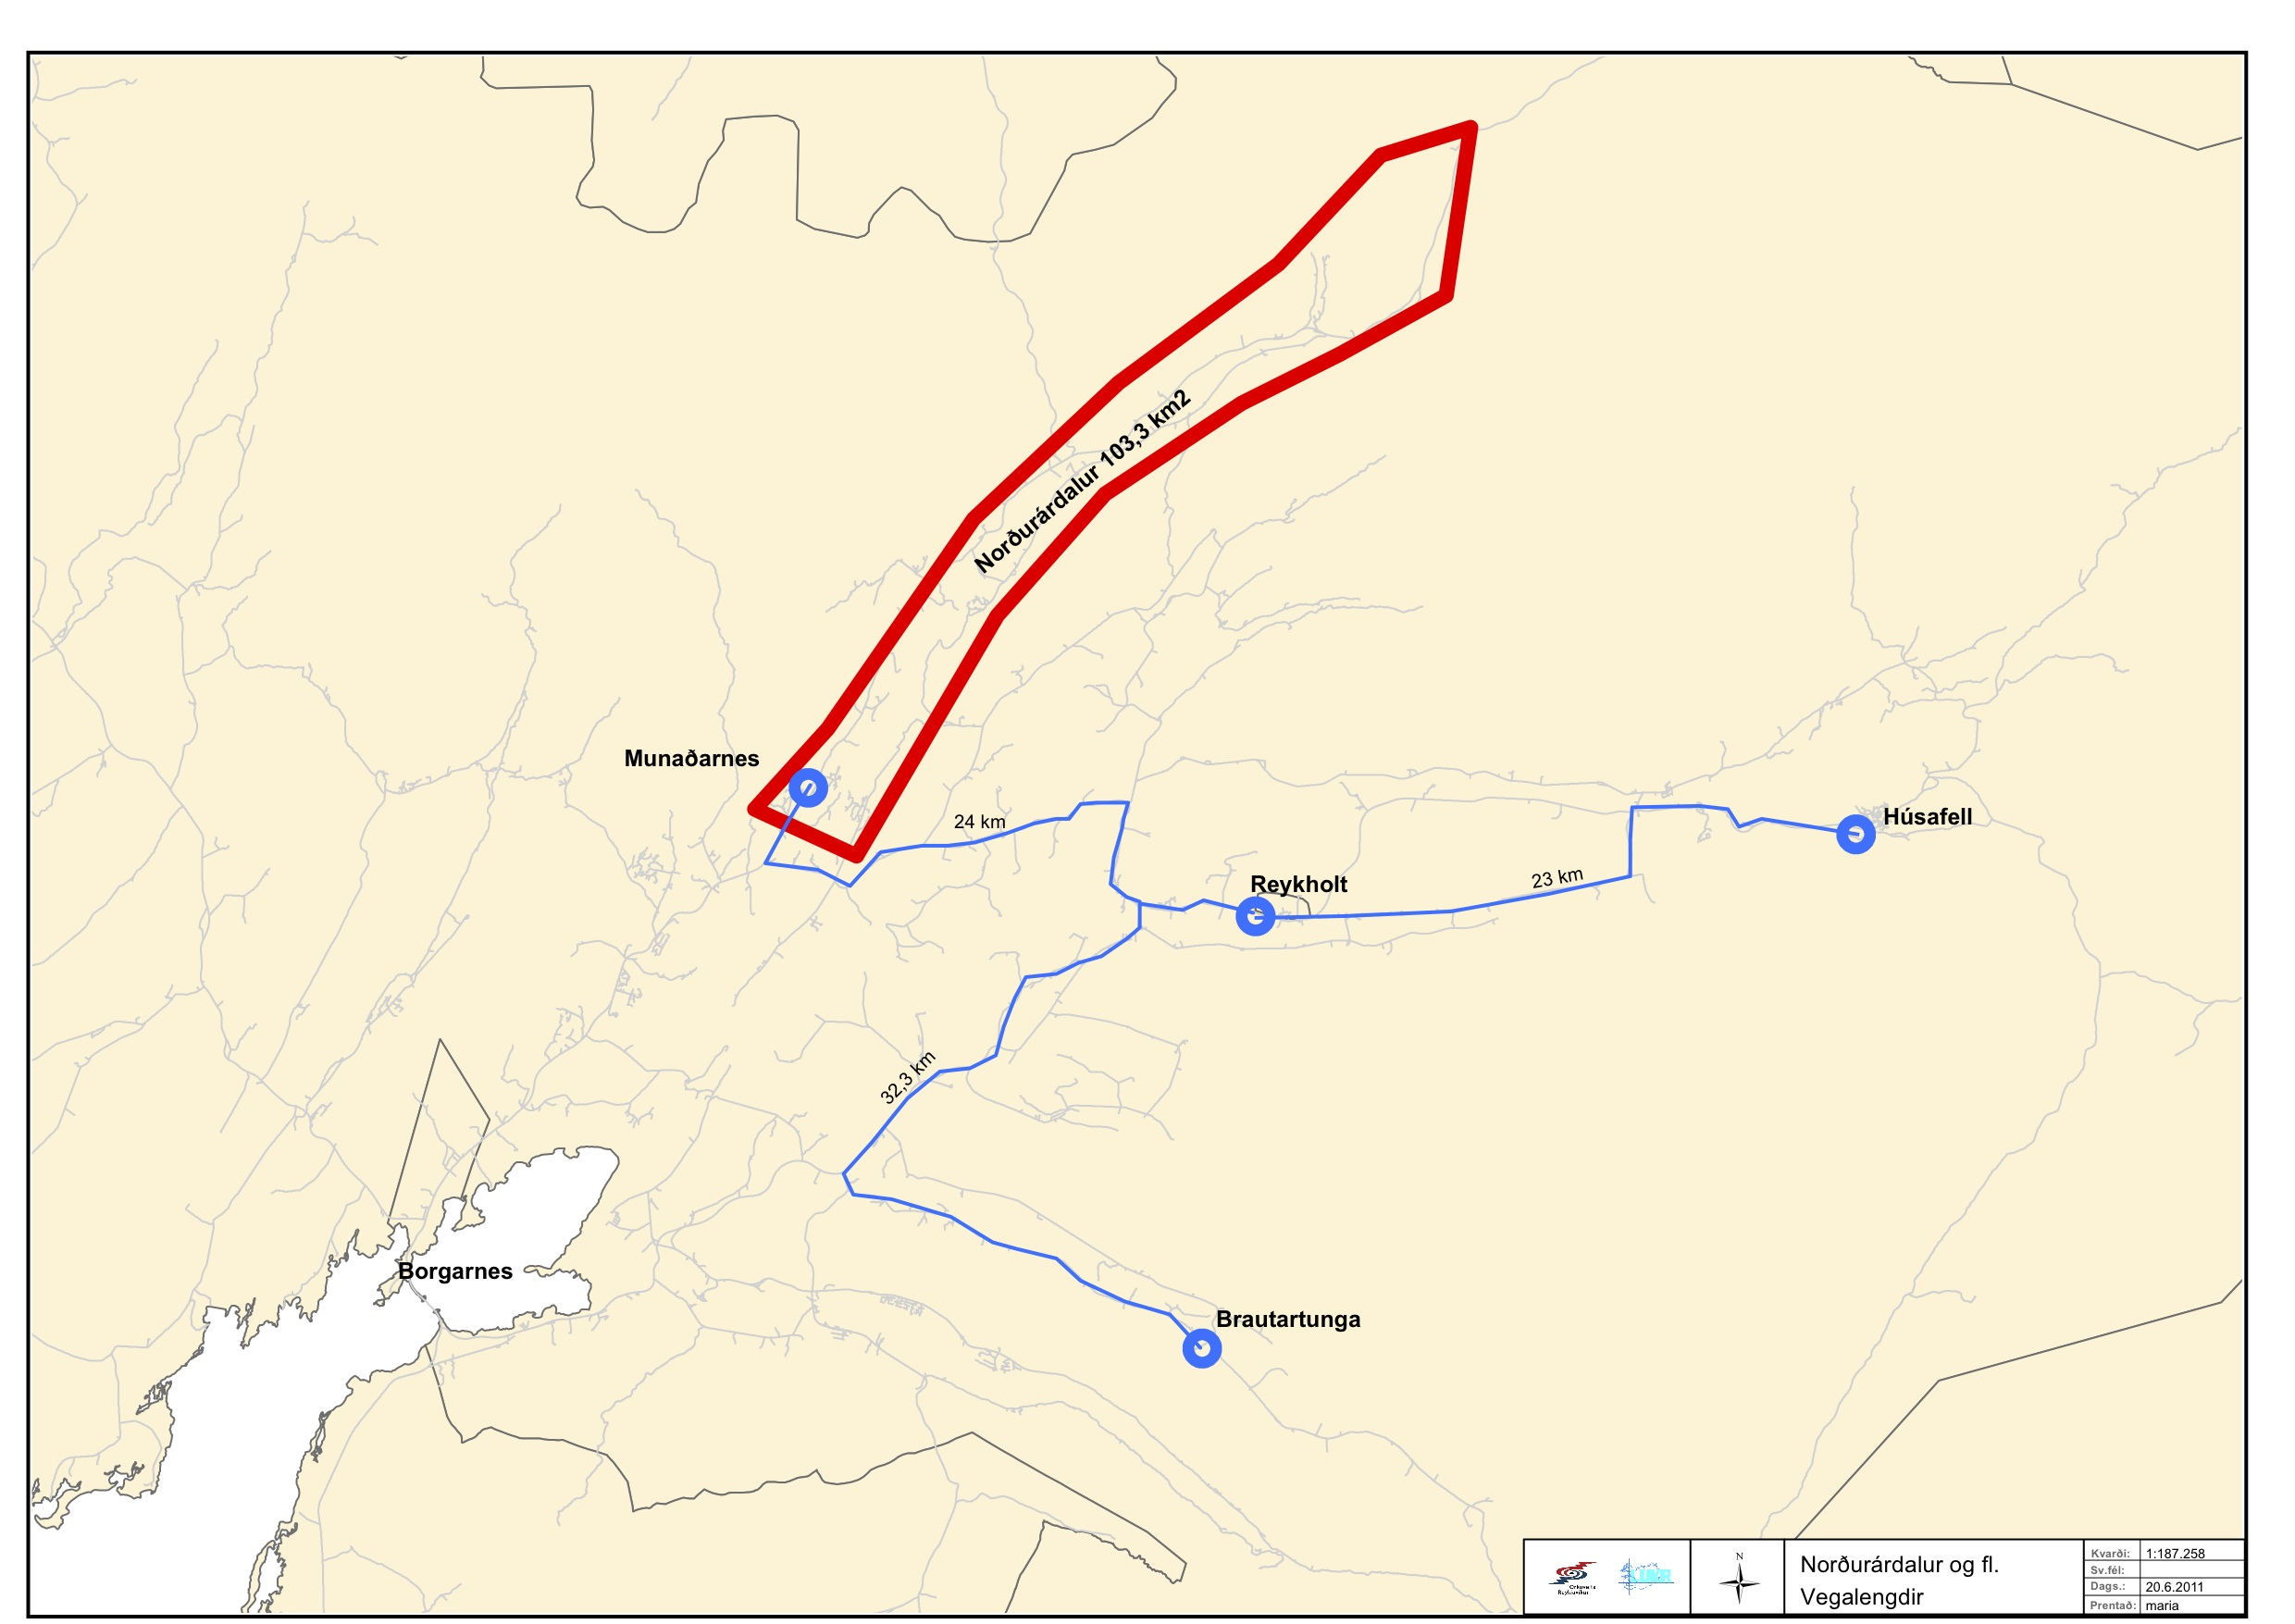
\includegraphics[width=6in]{nordu.jpg} 
%   \caption{ Borgarfjordur thermal field and Nordurardalur thermal system}
%   \label{fig:nordu}
%\end{figure}
%The Munardanes reservoir is situated in the Nordurardalur geothermal field. The later is located in west Iceland in the Borgarfjordur thermal field situated in the Borgarfjordur region. The Borgarfjordur thermal field is the largest low temperature geothermal field in Iceland. It comprises known thermal systems such as the Reykholt thermal system, the Bear thermal system, the Brautartunga thermal system, England thermal system, and the Husafell thermal system (Johannesson et al. 1980, Gunnlaugsson 1980). The natural discharge of the Borgarfjordur thermal system also called the Reykholtsdalur thermal system is estimated to 450$l/s$ of boiling water (Georgsson et al. 1984).  Within the Borgarfjordur thermal field, the Reykholf thermal system is by fare the largest thermal system with a total discharge of 400$l/s$ (Georgsson et al. 1980). The Nordurardalur thermal system is located north-west to the five major thermals systems mention above. It is a N-W long band of about 103 $km^{2}$ .
%
%\subsection{Geological setting}
%\begin{figure}[htbp] %  figure placement: here, top, bottom, or page
%   \centering
%   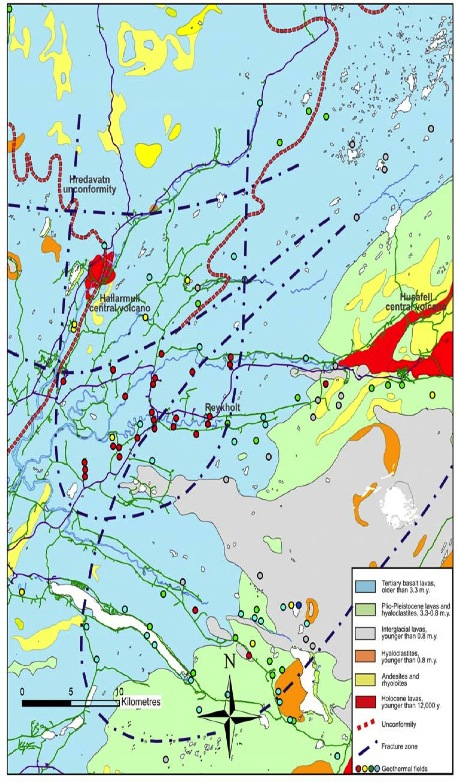
\includegraphics[width=4in]{bgeo.jpg} 
%   \caption{Geological map of Borgarfjordur thermal field}
%   \label{fig:bgeo}
%\end{figure}
%
%Upper tertiary ($>$3.3 Myr) basaltic lava flow constitute the basement of the Borgarfjordur region. This lava flow is characterised by a uniform lithology, either uniform texture or composition. The oldest rock being 14-15 Myrs. The bulk of this tertiary lava flow is made of tholeiites basaltic rock separated by minor clastic interbeds (Saemundsson 1979). The tholeiites basaltic lava pile is characterized by its content in sodium which is less than other basaltic rock. The Borgarfjordur thermal field is bounded from the east by the western volcanic rift zone and the snaefellnes volcanic zone from the west. The later present little or no rifting. Those two volcanic zones represent the origin of the tertiary lava flow.  However, the tholeiites content of the lava flow suggest that the lava flow is predominantly from the Sneafellsnes volcanic flank zone. \\
%\\
% Both unconformity and anticline structures are visible in the region. The later formed from rift relocation (Saemundsson, 1967). Recall that an anticline is defined as layers of sedimentary rock having the oldest strata in its core and forming a convex shape. An unconformity is a planar structure indicating a discontinuity in a geologicale structure due to erosive forces. The anticline axis is defined as the line of intersection of the perpendicular plane cutting the anticline in two symmetric parts. The Borganes anticline runs NE-SW (saemundsson 1977). The lava flow dip towards the Reykjanes-Langjokull rift zone to the east of the anticline axis. The Hredavatn unconformity is situated in north of Hredavatn lake. This unconformity indicate intense erosive forces acting in the borgarfjordur region.
%
%\subsection{Geophysical and hydrological setting}
%
%The geophysics of the region is characterised by the volcanism, the tectonic and the different forces affecting the earth crustal structure. The region is located between the Sneafellsnes volcanic flank and the Reykjanes-Langjokull volcanic rift. The later is made of the Reykjanes peninsula and the Western volcanic zone. The Reykjanes-Lanjokull rift is characterised by faulting resulting from tensional stress in the earth crust.  The Nordurardalur geothermal system is confined within the WNW-ESE, N-S  fractures zone   and between the Hradavatn unconformity and the Borganes anticline. An extinct central volcano is sitting within the Nordurardalur thermal system.\\
%The resistivity in Nordurardalur alternate between 20 and 100 $\Omega m$.  The 20 $\Omega m$ resistivity part is located in the lowest part of the Nordurardalur band and quickly 
%increase to 60 and 100 as we move North east. The value alternate to 30-40 then decrease to 20 before increasing to about 30 $\Omega m$.\\
%\\
%The geothermal water is of meteoric origin which as fallen as precipitation on the highland. The water percolate through fractures cracks or others pathways through the earth and is heated by regional heat flow. The flow pattern can be infer base on preview studies done in the main thermal systems in Borgafjordur. The Northeasterly faults are the main channels for the Nordurardalur thermal system and the seismicity in the region allows fractures to serve as flow path. The recharge zone is the Arnarvatnsheidi highland and the flow pattern is 
%
%\subsection{Proposed conceptual model of Borgarfjordur thermal filed}
%\begin{figure}[htbp] %  figure placement: here, top, bottom, or page
%   \centering
%   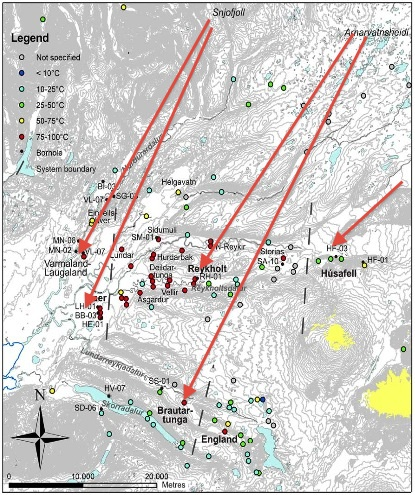
\includegraphics[width=5in]{flowp.jpg} 
%   \caption{Production well in Borgarfjordur thermal field with flow patterns of the main thermal systems}
%   \label{fig:flowp}
%\end{figure}
%Figure (\ref{fig:flowp}) indicates the flow patterns of the main thermal system in Borgarfjordur thermal field. The Reykholt and the Brautartungar thermal field recharge zone is located in the Arnarvatnsheidi high land. The Husafell thermal system recharge zone is located east to the Arnarvatnsheidi high land. For those tree systems, the easterly and north easterly faults and fractures allows the meteoric water to percolate at depth, acting as flow channels. The Nordurardalur system can be seen as a part of the Bear thermal system. The recharge zone is situated in the surrounding  of Snjofjoll, latitude 64 Degree 59 $mn$ $N$, longitude 21 Degree 11 $mn$ W. The $NS$ fractures act as flow channels, where the water flows by the Hallarmuli extinct central volcanoes. \\
%\\
%Heat is transfer by conduction through the earth crust from the Snaefellsnes volcanic flank and the Reykjaness-Langjokull volcanic rift zone. Heat is convected by the hot water though the fracture and fault systems at depth. The integrity of the fracture/fault system are maintain by the seismicity in the region. They also act as barriers zone. The salinity of water is the highest in the Bear thermal system as well as in the Nordurardalur system. As we move away from the Bear system the salinity decrease, being the lowest in Husafell thermal system.
%

%%%%%%%%%%%%%%%%%%%%%%%%%%%%%%%%%%%%%%%%%%%%%%%%%%%%%%%%%%

\subsection{Lumped parameter modelling of well $MN 08$ in Munadarnes in Nordurardalur}
Well $MN 8$ was drilled in 2003 east of the summer house lacerated in Munadarnes. The  $900 m$ deep low temperature well own by Reykjavik Energy was drilled after a survey revealed a temperature gradient of $250\,^{\circ}{\rm c}/km$ \cite{Hjartarson2003}. Testing and measurement of the well from February to March 2003 revealed that the temperature of the well is approximate $ 90\,^{\circ}{\rm c}$ and the main main feed zone is located at about $440 m$ \cite{Hjartarson2003}.\\


\begin{figure}[H] %  figure placement: here, top, bottom, or page
   \centering
   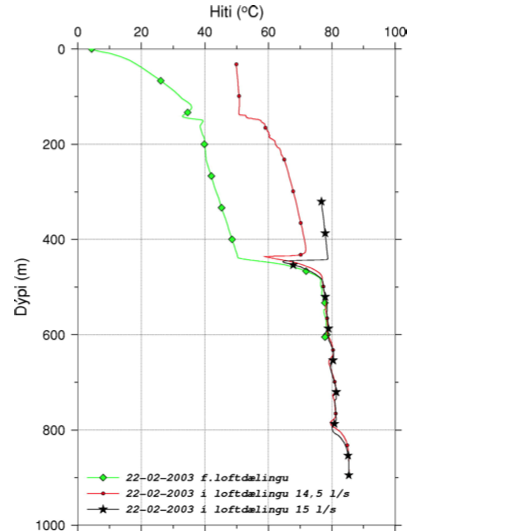
\includegraphics[width=4in]{tme.png} 
   \caption{Temperature measurement in well $MN 8$ \cite{Hjartarson2003}}
   \label{fig:example}
\end{figure}

Water level, pressure, temperature, production rate were monitored from January 2008 to December 2010. The well was initially drilled in 2003 with an initial water level of $35 m$. The first data set was rearrange by eliminating outliers, that is data points that are numerically distant from the rest of the data. The new data set was however still spread out.  Despite the spreading we  obtain a satisfactory  two tanks open model which was later used for future prediction. 

\subsubsection{Data processing and simulation}
The data obtained was very spread out. One possible explanation was that the data was contaminated by outliers.

\begin{table}[H]
	\begin{center}
		\begin{tabular}{|c|c|c|r|}
		\hline
			water level in $(m)$ & production in $(l/s)$ & date in $(YYY/mm/dd)$& time in $(hh:mm)$  \\ \hline
			$118.8$ &$8.8$  &$2010/03/29$  & $11:23$      \\ 
			$83.6$ & $7.1$ & $2010/01/06$  & $12:09$     \\ 
			$78.6$ &$8.4$ & $2009/12/01$   & $13:50$    \\ 
			$76.6$ &$8.4$ & $2010/02/15$    & $13:33$   \\ 
			$68.6$&$5.2$   & $2009/02/11$    & $10:20 $ \\ 
			$68.6$&$7.3$   & $2010/11/29$    & $14:22 $ \\ 
			$66.6$&$3$   & $2009/10/19$    & $9:40 $ \\ 
			$66.6$&$9$   & $2010/03/22$    & $13:55 $ \\ 
			$66.6$&$9$   & $2010/03/24$    & $20:09 $ \\ 

			\hline
		\end{tabular}
		\caption{Outliers removed from the simulated data}
		\label{tab:out}
	\end{center}
\end{table}


\begin{figure}[H] %  figure placement: here, top, bottom, or page
   \centering
   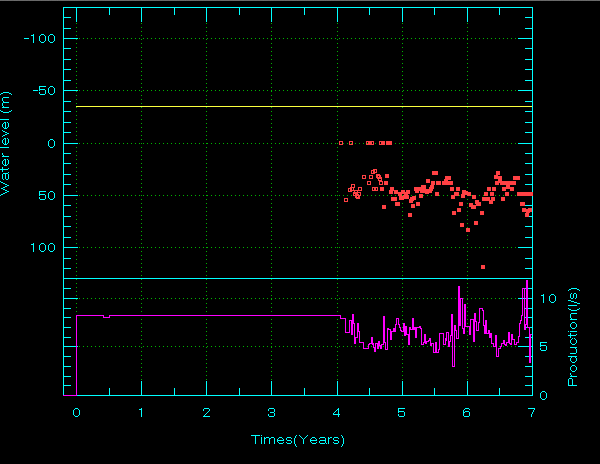
\includegraphics[width=4in]{idata.png}  
   \caption{Original data set}
   \label{fig:data}
\end{figure}

\begin{figure}[H] %  figure placement: here, top, bottom, or page
   \centering
   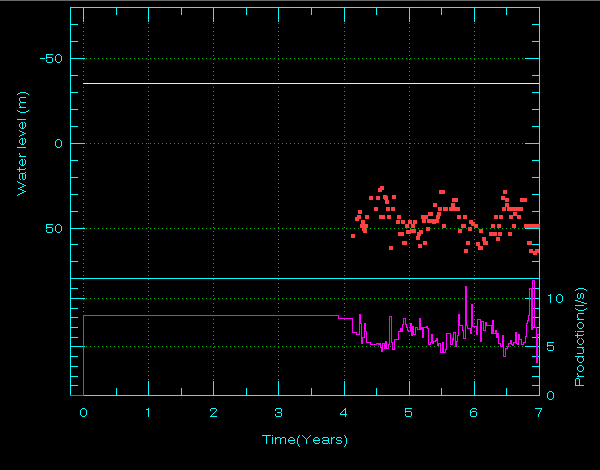
\includegraphics[width=4in]{ndata.png}  
   \caption{Data set obtained after removing the outliers in table \ref{tab:out} }
   \label{fig:data}
\end{figure}

\begin{figure}[H] %  figure placement: here, top, bottom, or page
   \centering
   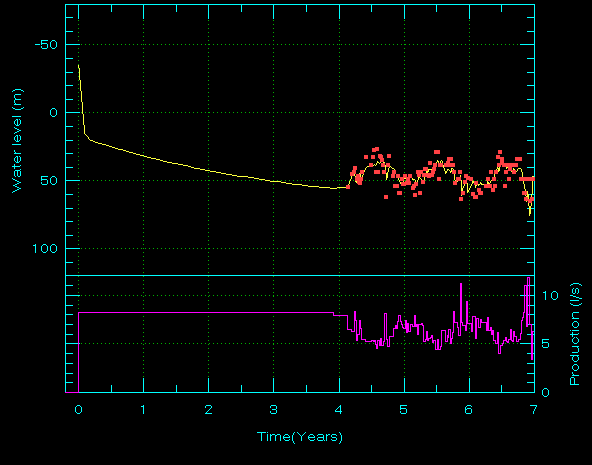
\includegraphics[width=4in]{twoto.png}  
   \caption{two tanks open model simulation }
   \label{fig:to}
\end{figure}




\begin{table}[H]%
\label{model}\centering 

\begin{tabular}{|c|l|c|c|c|}
\hline                                         
 Model number                 & 1           & 2         & 3  & 4        \\ %\toprule
\hline
Number of tanks              & 1           & 1        & 2   & 2 \\  %\midrule
\hline
Number of parameters  & 2           & 4        & 6     &  8   \\
\hline
Model types                     &Closed &Open& Closed & Open\\
\hline
$A_{1} $                           & 0    & 10.14  & 10.85 &17.8979            \\
\hline
$L_{1}$                            &  0      &  0.8   &  1.16& 2.82     \\
\hline
$A_{2}$                            &    0   &      0      & 0    &  0.17      \\
\hline
$L_{2}$                            &    0       & 0     & 0  & 0.025 \\
\hline
$B$  $(10^{-3})$              & 154.4  & 0  &  41.3 & 0 \\
\hline
$\kappa_{1} $                 & 1741.4 & 26.52& 24.68&14.88   \\
\hline
$\kappa_{2} $                 &0  & 0  & 6487.2&   1593.36        \\
\hline
$\kappa_{3}$                &   0 &   0   & 0 & 0 \\ 
\hline
$\sigma_{1}(10^{-6})$ &0 &  8     &  10.83& 16.8         \\
\hline
$\sigma_{2}(10^{-6})$  &   0 &   0&  0      &  15.2     \\
\hline
$RMS(m)$                       & 12.26 & 7.46 &   6.65 & 5.91           \\  %\bottomrule
\hline
$STD(m)$                          &12.31 &7.52 & 6.73&6.01   \\
\hline
$R^{2} (\%)$                      &0.00  &30.6  &44.88 & 56.46\\     
\hline  
\end{tabular}
\caption{Parameters of the lumped models for the production well $MN 8$ in Munardanes}
\label{tab:re}
\end{table}  



\begin{table}[H]%

\label{model}\centering 

\begin{tabular}{|c|l|}
\hline                                         
 Porosity $\phi$                 & 0.15        \\ %\toprule
\hline
depth $H (m)$              & 900       \\  %\midrule
\hline
gravity $(m/s^{-2})$  & 9.81        \\
\hline
Water compressibility  $C_{w} ( 10^{-10} Pa^{-1})$ & 4.6534 \\
\hline
Rock compressibility  $C_{r} (10^{-10} Pa^{-1})$ &3.3          \\
\hline
$s_{c} ( 10^{-7} kg/m^{3}Pa)$ &  3.4        \\
\hline
$s ( 10^{-5}kg/m^{3}Pa)$       &    1.7         \\
\hline  
\end{tabular}
\caption{Storativity estimation for  well $MN 8$ in Munardanes}
\label{tab:st}
\end{table}  
If the reservoir was confined, it would cover an area of about $525.5 km^{2}$ which is too large compared to the geothermal field. On the other hand, in the  unconfined case, the total area for the reservoir is about $10.5 km^{2}$. We therefore conclude that the reservoir is unconfined, with an approximated area of $10.5 km^{2}$. The permeability is estimated at about $69.8$ $mDarcy$. 



\subsubsection{ Prediction with reinjection}
Based on the analytical pressure response given in equation (\ref{eq:o}), a 20  years future prediction is given for different production scenarios.
% The storativity for an unconfined and a confined geothermal reservoir was given in section 2. For an average temperature of 86 degree c table \ref{tab:st} gives the storativity for confined $(s_{c})$ and unconfined $(s)$ reservoir.
%
%\begin{table}[H]%
%
%\label{model}\centering 
%
%\begin{tabular}{|c|l|}
%\hline                                         
% Porosity $\phi$                 & 0.15        \\ %\toprule
%\hline
%depth $H (m)$              & 900       \\  %\midrule
%\hline
%gravity $(m/s^{-2})$  & 9.81        \\
%\hline
%Water compressibility  $C_{w} ( 10^{-10} Pa^{-1})$ & 4.6534 \\
%\hline
%Rock compressibility  $C_{r} (10^{-10} Pa^{-1})$ &3.3          \\
%\hline
%$s_{c} ( 10^{-7} kg/m^{3}Pa)$ &  3.4        \\
%\hline
%$s ( 10^{-5}kg/m^{3}Pa)$       &    1.7         \\
%\hline  
%\end{tabular}
%\caption{Storativity estimation for  well $MN 8$ in Munardanes}
%\label{tab:st}
%\end{table}  
%If the reservoir was confined, it would cover an area of about $525.5 km^{2}$ which is too large compared to the geothermal field. On the other hand, in the  unconfined case, the total area for the reservoir is about $10.5 km^{2}$. We therefore conclude that the reservoir is unconfined, with an approximated area of $10.5 km^{2}$. The permeability is estimated at about $6.98.10^{-10} m^{2}$ or $69.8$ $mDarcy$. Based on the analytical pressure response given in equation (\ref{eq:o}), a 20  years future prediction is given in figure \ref{fig:f} for different production scenario.


\begin{figure}[H] %  figure placement: here, top, bottom, or page
   \centering
   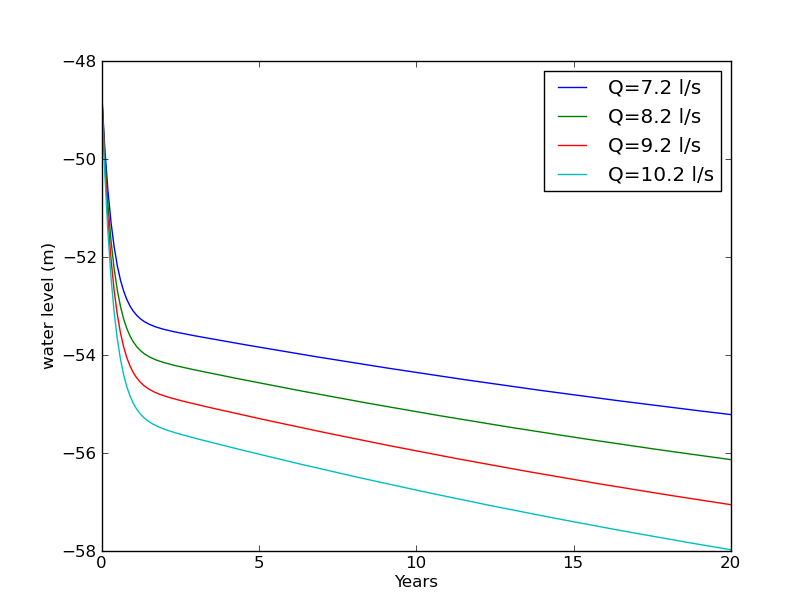
\includegraphics[width=4in]{future.png} 
   \caption{ 20 years future prediction from 2010, without reinjection}
   \label{fig:f}
\end{figure}

\begin{figure}[H] %  figure placement: here, top, bottom, or page
   \centering
   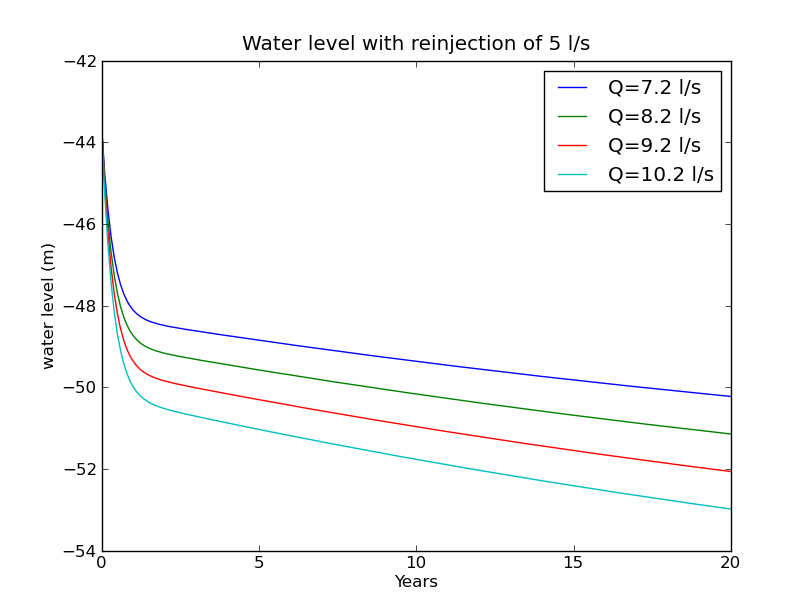
\includegraphics[width=4in]{r5.png} 
   \caption{20 years production with reinjection scenario for 5 $l/s$ injection rate at the start of production}
   \label{fig:r5}
\end{figure}

\begin{figure}[H] %  figure placement: here, top, bottom, or page
   \centering
   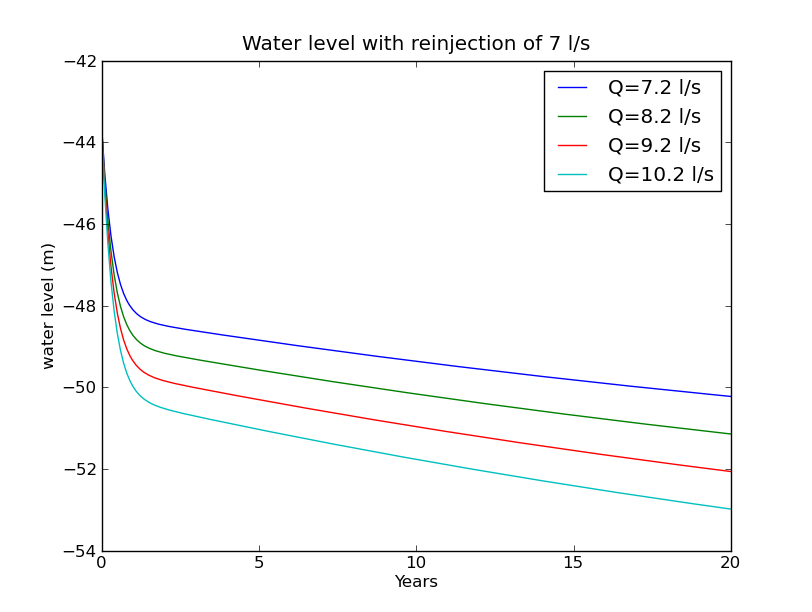
\includegraphics[width=4in]{r7.png} 
   \caption{20 years production with reinjection scenario for 7 $l/s$ injection rate at the start of production}
   \label{fig:r7}
\end{figure}

\begin{figure}[H] %  figure placement: here, top, bottom, or page
   \centering
   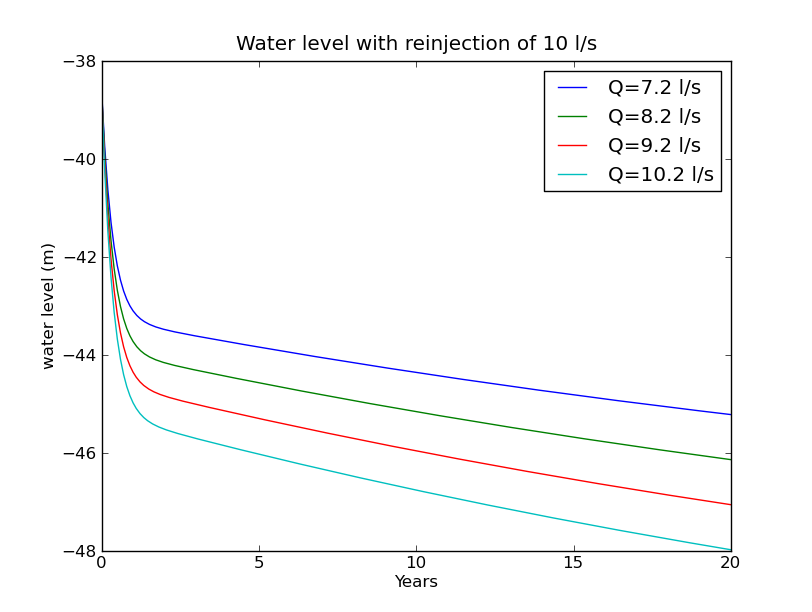
\includegraphics[width=4in]{10ls.png} 
   \caption{ 20 years production with reinjection scenario for 10 $l/s$ injection rate at the start of production}
   \label{fig:10ls}
\end{figure}


Figure \ref{fig:f} shows a 20 years prediction with production rate of $7.2$ $l/s$, $8.2$ $l/s$, $9.2$ $l/s$ and $10.2$ $l/s$.  Figure \ref{fig:r5}, \ref{fig:r7} and \ref{fig:10ls} shows the change in water level over a period of 20 years with three injection scenarios of water at 5, 7 and $10$ $l/s$ reinjection rate. The reinjection scenarios assumed that reinjection started at the beginning of of 2004. The minimum and maximum production rate are assumed to be $7.2$ $l/s$, $10.2$ $l/s$ respectively. As seen water leveel increases significantly with injection. However due to the cold nature of the injected water some cooling can be induce.\\
\\
\subsubsection{ Location of injection well and cooling of production well}\\

Based of a theoretical model of a one dimension flow channel, along a fracture zone, The temperature of a production well is given by \cite{Axelsson2005}:

\begin{equation}\label{eq:cool}
T(t) = T_{0}-\frac{q}{Q}(T_{0}-T_{i})\left (  1-\erf\left(    \frac{kxh}{c_{w}q\sqrt{\kappa(t-x/\beta)}}}       \right)        \right)
\end{equation}
with $T(t)$ the production fluid temperature, $T_{0}$ the undisturbed reservoir temperature, $T_{i}$ the injection temperature, $q$ and $Q$ the rate of injection and production respectively, $k$ the thermal conduction of the reservoir rock, $\kappa$ the thermal diffusivity, $x$ the distance between injection and production wells and
\begin{equation}
\beta = \frac{qc_{w}}{<\rho c>_{f}hb} \nonumber
\end{equation}
with 
\begin{equation}
<\rho c>_{f} =\rho_{w}c_{w}+\rho_{r}c_{r}(1-\phi) \nonumber
\end{equation}
the volumetric heat capacity of the material in the flow channe. $\rho$ and $c$ are density and heat capacity respectively, with indices $w$ and $r$ standing for water and rock.

\begin{figure}[H] %  figure placement: here, top, bottom, or page
   \centering
   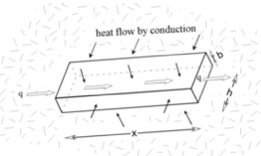
\includegraphics[width=4in]{fc.png} 
   \caption{model of flow channel for cooling of production well during injection \cite{Axelsson2005}}
   \label{fig:fc}
\end{figure}

Assume a one dimensional channel with $h = 29$ $m$, $b=7$ $m$ and porosity $\phi = 0.15$. The injection water temperature is $T_{i}=20\,^{\circ}{\rm c}$ and the reservoir temperature $T_{0}=86\,^{\circ}{\rm c}$. The thermal conductivity $k=2$. The specific heat capacity and the density are given by Stoppa et. al as a function of temperature \cite{Waj05}. The theoretical cooling of well $MN 08$ in Munadarnes during a 10 years reinjection scenario is given bellow:


\begin{figure}[H] %  figure placement: here, top, bottom, or page
   \centering
   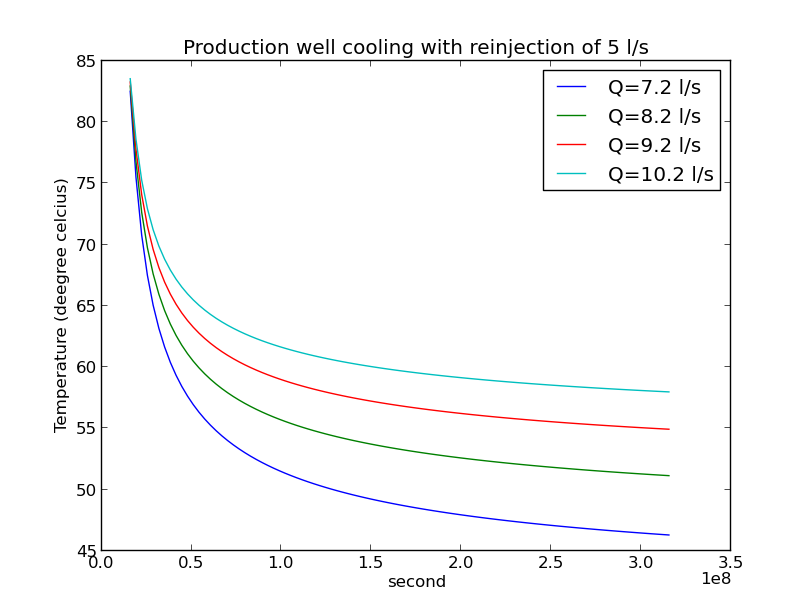
\includegraphics[width=4in]{5ls500m.png} 
   \caption{Production well cooling for injection well located at $500$ $m$ from production well. Injection rate 5 $l/s$}
   \label{fig:one}
\end{figure}

\begin{figure}[H] %  figure placement: here, top, bottom, or page
   \centering
   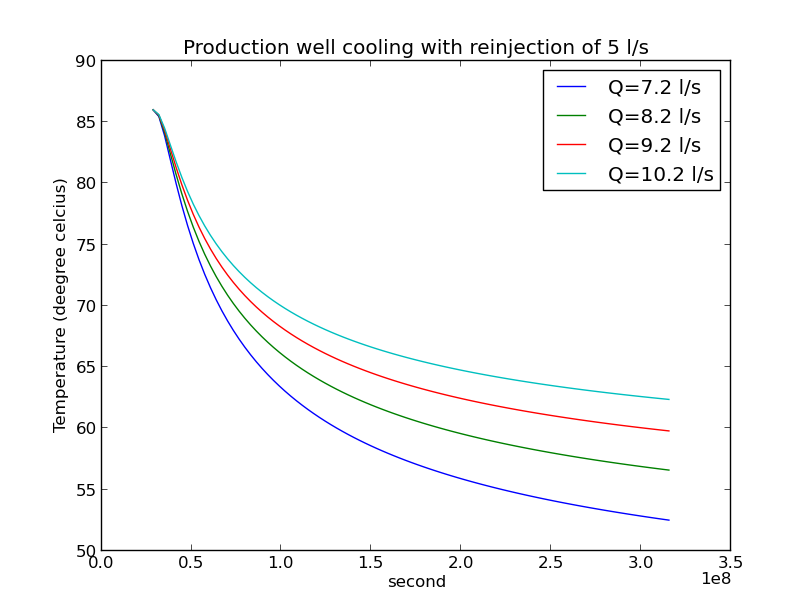
\includegraphics[width=4in]{5ls1km.png} 
   \caption{Production well cooling for injection well located at $1$ $km$ from production well. Injection rate 5 $l/s$}
   \label{fig:two}
\end{figure}

\begin{figure}[H] %  figure placement: here, top, bottom, or page
   \centering
   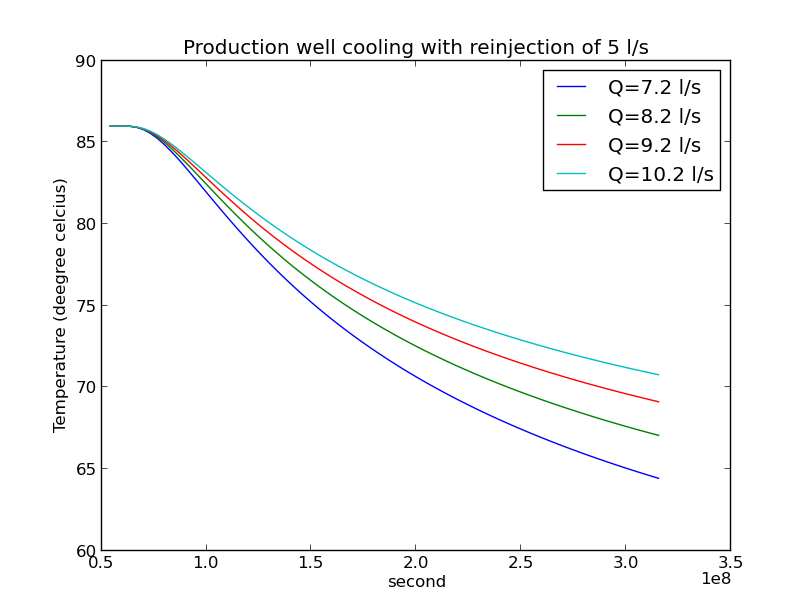
\includegraphics[width=4in]{5ls2km.png} 
   \caption{Production well cooling for injection well located at $2$ $km$ from production well. Injection rate 5 $l/s$}
   \label{fig:three}
\end{figure}


\begin{figure}[H] %  figure placement: here, top, bottom, or page
   \centering
   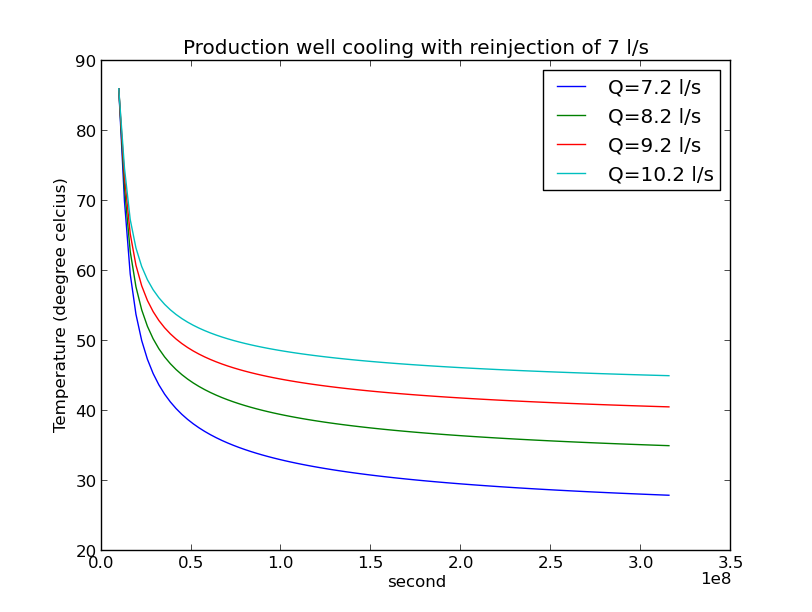
\includegraphics[width=4in]{7ls500m.png} 
   \caption{Production well cooling for injection well located at $500$ $m$ from production well. Injection rate 7 $l/s$}
   \label{fig:four}
\end{figure}

\begin{figure}[H] %  figure placement: here, top, bottom, or page
   \centering
   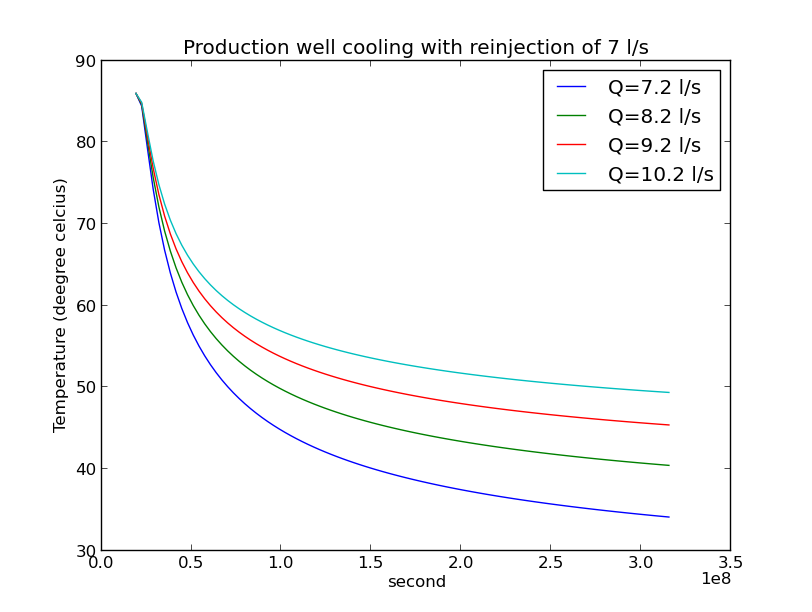
\includegraphics[width=4in]{7ls1km.png} 
   \caption{Production well cooling for injection well located at $1$ $km$ from production well. Injection rate 7 $l/s$}
   \label{fig:five}
\end{figure}

\begin{figure}[H] %  figure placement: here, top, bottom, or page
   \centering
   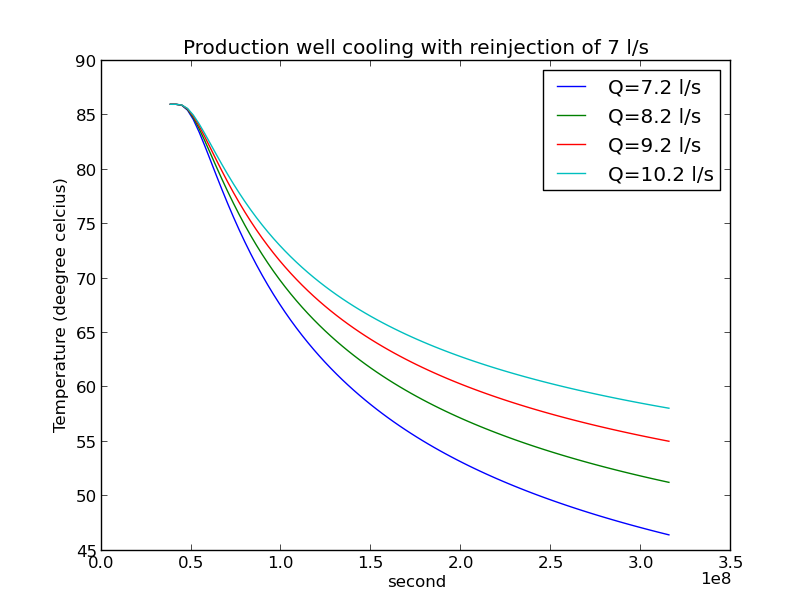
\includegraphics[width=4in]{7ls2km.png} 
   \caption{Production well cooling for injection well located at $2$ $km$ from production well. Injection rate 7 $l/s$}
   \label{fig:six}
\end{figure}
As seen from Figures \ref{fig:one} to \ref{fig:six} the temperature of the production well decrease when the injection well is closer to the production well. At a distance of 2 $km$ the cooling effect is attenuated. The production well temperature is lower for higher injection rate. As the production rate is increased so is the temperature of the production well during injection.





% Chapter 

\chapter{Conclusion and future work} % Main chapter title

\label{Chapter5} % For referencing the chapter elsewhere, use \ref{Chapter1} 

\lhead{Chapter 5. \emph{Conclusion and future work}} % This is for the header on each page - perhaps a shortened title

%----------------------------------------------------------------------------------------


%\section{ Discussions, conclusion and future work}
The focus of this thesis was to model a low temperature geothermal system by using two dynamical methods:  A lumped parameter modelling for simulating pressure change and an analytical method for determining the velocity of cold water movement during injection. A data set was provided by Reykjavik Energy for lumped parameter simulation of well $MN 8$. The sample data consisted of water level (Pressure) and production rate from 2003 to 2008. This data appears to to be spread out, possibly due to measurement error. Using a two tanks open model the simulation was performed with a coefficient of determination of about 56 $\%$. From the lumped parameter modelling of well $MN 8$ located in Munadarnes in west Iceland, the Munadarnes reservoir permeability  was estimated to be about 68.8 $mD$. Most geothermal system permeability is in the range of $1-100$ $mD$.
The reservoir size was estimated to be about 10.5 $km^{2}$, with unconfined recharge mechanism. \\

Based on simulation parameters from the lumped parameters modelling, a 20 years production scenario without and with reinjection revealed that reinjecrion mitigates pressure drown down due to production. For a current production rate of $8.2$ $l/s$ and a reinjection water of $20 \,^{\circ}{\rm c}$ a  scenario without injection shows that over 20 years the water level will drop by 7.4 $m$. However with reinjection at a rate of 5 $l/s$ the water level with decrease by 2.4 $m$. Renjecting cold water into a hot reservoir can cause the reservoir rock to cool down. To mitigate this cooling effect the injection well must be placed within the production zone and at a few $km$ from the production well. From a theoretical solution of fluid flow in a one dimensional channel the cooling of well $MN 08$ was studied over 10 years. The cooling of well $MN 08$ depends on three factors: The injection rate $q$, the production rate $Q$ and the distance between the production well and the injection well.  The injection rate was set at 5 $l/s$ while the production rate varies from $7.2$ to $10.2$ $l/s$. From an initial reservoir temperature of $86 \,^{\circ}{\rm c}$ the temperature of the reservoir over 10 years was about $58\,^{\circ}{\rm c}$ for a production rate of $10.2$ $l/s$ and a distance of 500 $m$ between production well and injection well. When the distance between production and injection well was increased to 2 $km$ the reservoir temperature over 10 years was about $71 \,^{\circ}{\rm c}$.\\
For the same injection rate of 5 $l/s$ and production rate of 7.2 $l/s$ the temperature of the well was $46 \,^{\circ}{\rm c}$ and $64 \,^{\circ}{\rm c}$ for a distance of 500 $m$ and 2 $km$ respectively. This results shows that to minimise the cooling effect of reinjection the injection well must be place at few $km$ from the production well within the production zone. increase in production rate also mitigate cooling during injection of cold water. Accurate position of injection well must however be determined after a tracer test experiment.\\
\\
The velocity of the cold injected water was also derived from the theory of hyperbolic conservations laws. The result present in this  work was compared with the one obtained by Stoppa et al. A relative error of $10^{-3}$ was observed between the two results. The numerical evaluation of the analytical expressions was derive using a simple numerical integration scheme: The trapezoidal rule.\\

This work can naturally be extended to include a lumped parameter modelling of hight temperature reservoirs. In this case the two phase flow nature of high temperature wells must be included. The injection of cold water in two phase flow reservoirs can also be studied. Due to the complexity of two phase flow a numerical method might be necessary. 

%----------------------------------------------------------------------------------------
 
%\input{./Chapters/Chapter5} 
%\input{./Chapters/Chapter6} 
%\input{./Chapters/Chapter7} 

%----------------------------------------------------------------------------------------
%	THESIS CONTENT - APPENDICES
%----------------------------------------------------------------------------------------

\addtocontents{toc}{\vspace{2em}} % Add a gap in the Contents, for aesthetics

\appendix % Cue to tell LaTeX that the following 'chapters' are Appendices

% Include the appendices of the thesis as separate files from the Appendices folder
% Uncomment the lines as you write the Appendices

%% Appendix A

\chapter{Appendix Title Here} % Main appendix title

\label{AppendixA} % For referencing this appendix elsewhere, use \ref{AppendixA}

\lhead{Appendix A. \emph{Appendix Title Here}} % This is for the header on each page - perhaps a shortened title

Write your Appendix content here.
%\input{./Appendices/AppendixB}
%\input{./Appendices/AppendixC}

\addtocontents{toc}{\vspace{2em}} % Add a gap in the Contents, for aesthetics

\backmatter

%----------------------------------------------------------------------------------------
%	BIBLIOGRAPHY
%----------------------------------------------------------------------------------------

%\label{Bibliography}


\lhead{\emph{Bibliography}} % Change the page header to say "Bibliography"

\bibliography{main}
\bibliographystyle{plain}
%\bibliographystyle{unsrtnat} % Use the "unsrtnat" BibTeX style for formatting the Bibliography

%\bibliography{Bibliography} % The references (bibliography) information are stored in the file named "Bibliography.bib"


\end{document}  